\documentclass[12pt]{report}

\usepackage{ctex}
\usepackage{xeCJK}
\usepackage{fontspec}
\usepackage{xunicode}
\usepackage{tikz}
\usepackage{amsmath}    % need for subequations
\usepackage{graphicx}   % need for figures
\usepackage{verbatim}   % useful for program listings
\usepackage{color}      % use if color is used in text
\usepackage{subfigure}  % use for side-by-side figures
\usepackage{hyperref}   % use for hypertext links, including those to external documents and URLs

% don't need the following. simply use defaults
\setlength{\baselineskip}{16.0pt}    % 16 pt usual spacing between lines

\setlength{\parskip}{\medskipamount}
\setlength{\parindent}{0pt}
%% \setlength{\parskip}{3pt plus 2pt}
%% \setlength{\parindent}{20pt}
\setlength{\oddsidemargin}{0.5cm}
\setlength{\evensidemargin}{0.5cm}
\setlength{\marginparsep}{0.75cm}
\setlength{\marginparwidth}{2.5cm}
\setlength{\marginparpush}{1.0cm}
\setlength{\textwidth}{150mm}

\hypersetup{
  colorlinks=true,
  linkcolor=black
}

\begin{comment}
\pagestyle{empty} % use if page numbers not wanted
\end{comment}

\title{算法学习笔记}
\author{黄剑}
\date{\today}

% \includeonly{chapter_camp,chapter_leetcode}

% above is the preamble

\begin{document}
\maketitle
该文档是我学习算法过程中记录的笔记。
我把她分享出来,希望对正在学习算法的同学有所帮助。
最新版本可以从 \href{https://github.com/mdgsf/justcoding}{https://github.com/mdgsf/justcoding} 下载。
如果发现了错误,欢迎给我发邮件 1342042894@qq.com,或者直接在 github 上发 issue 也行。

\tableofcontents
\chapter{算法训练营学习笔记}

\newpage
\section{预习周}

\newpage
\section{第 1 课}

\subsection{第 2 课 | 训练准备和复杂度分析}

\subsubsection{开发环境}

\begin{quote}
工欲善其事,必先利其器
\end{quote}

每个人最好都有一个自己擅长的编辑器,这会让你的开发事半功倍。
我自己是使用\textbf{Vim}和\textbf{VSCode}。你要是不知道
使用哪个好,那就用\textbf{VSCode}准没错。

那怎么学习呢?直接在 Google 搜索 Top tips for VSCode

\subsubsection{时间复杂度}

\begin{itemize}
  \item O(1),Constant Complexity 常数复杂度,最佳,比如 Hash 表,缓存等。
  \item O($log_2 n$),Logarithmic Complexity 对数复杂度,
    仅次于常数复杂度,如二分查找、二叉搜索树等。
  \item O(n),Linear Complexity 线性复杂度,如大多数遍历操作。
  \item O(nlogn) 快速排序时间复杂度
  \item O(n$^{2}$) N square Complexity 平方,双重 for 循环
  \item O(n$^{3}$) N cubic Complexity 立方, 3 重 for 循环
  \item O(2$^{n}$),O(3$^{n}$),O(k$^{n}$) Exponential Growth 指数,
    递归的时间复杂度
  \item O(n!) 阶乘时间复杂度
\end{itemize}


\subsection{学习总结}

其实预习周里,覃超老师教的东西才是最有用的。 
``五毒神掌''这样的方法可以说是颠覆了自己的认知。 
自己以前一直都是想要自己去想题目的解决方法, 
结果可想而知,自然是碰到了很多的困难和挫折。 
毕竟你要是能想出那么精妙的算法的话,你都能拿图灵奖了。
所以学算法的第一步就是要先清楚的给自己划定一条边界:
你是要学习算法而不是要去 发明创造一个新的算法。
其实也很容易理解,你要是没有学习过加减乘除,
让你自己去发明加减乘除,试问又有几个人能够办到。
我们更多的时候,是站在前人的基础上。牛顿曾说过:
\begin{quote}
``我之所以能 成功,是因为我站在巨人的肩膀上''
\end{quote}
所以对于我们普通人而言,你更多的是需要认真学习。

\newpage
\section{第 01 周}

\subsection{第 3 课 | 数组、链表、跳表}

\subsubsection{脑图}

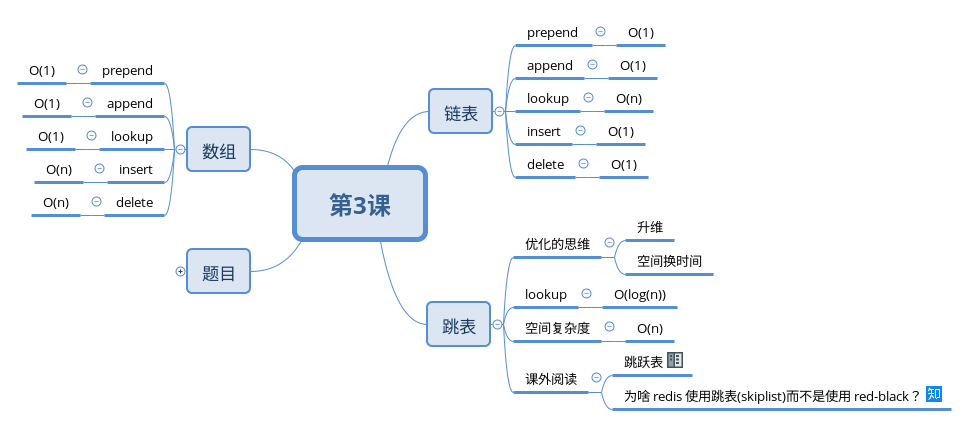
\includegraphics[width=170mm,height=80mm]{images/第3课.png}

\subsubsection{题目}

\paragraph{Array 实战题目}

\begin{itemize}
  \item \hyperref[leetcode:11]{11. 盛最多水的容器}
  \item \hyperref[leetcode:283]{283. 移动零}
  \item \hyperref[leetcode:70]{70. 爬楼梯}
  \item \hyperref[leetcode:15]{15. 三数之和}
\end{itemize}

\paragraph{Link List 实战题目}

\begin{itemize}
  \item \hyperref[leetcode:206]{206. 反转链表}
  \item \hyperref[leetcode:24]{24. 两两交换链表中的节点}
  \item \hyperref[leetcode:141]{141. 环形链表}
  \item \hyperref[leetcode:142]{142. 环形链表 II}
  \item \hyperref[leetcode:25]{25. K 个一组翻转链表}
\end{itemize}

\paragraph{课后作业}

\begin{itemize}
  \item \hyperref[leetcode:26]{26. 删除排序数组中的重复项}
  \item \hyperref[leetcode:189]{189. 旋转数组}
  \item \hyperref[leetcode:21]{21. 合并两个有序链表}
  \item \hyperref[leetcode:88]{88. 合并两个有序数组}
  \item \hyperref[leetcode:1]{1. 两数之和}
  \item \hyperref[leetcode:283]{283. 移动零}
  \item \hyperref[leetcode:66]{66. 加一}
\end{itemize}

\subsection{第 4 课 | 栈、队列、优先队列、双端队列}

\subsubsection{脑图}

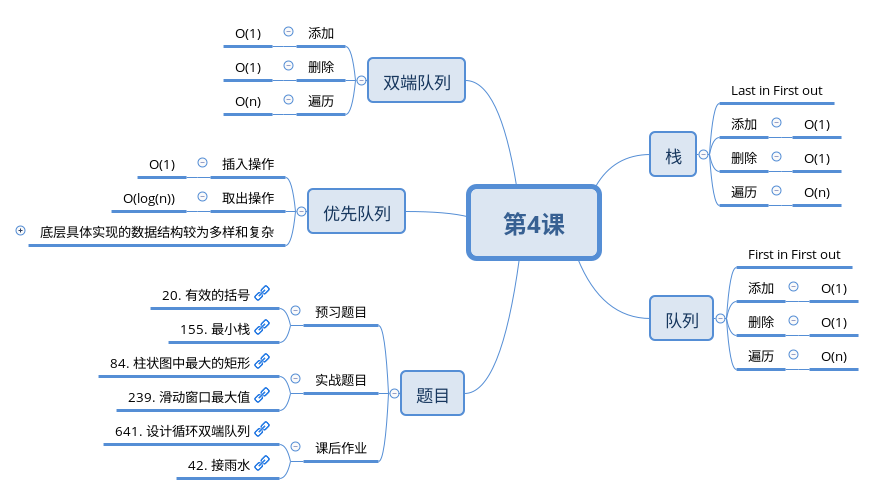
\includegraphics[width=170mm,height=80mm]{images/第4课.png}

\subsubsection{题目}

\paragraph{预习题目}

\begin{itemize}
  \item \hyperref[leetcode:20]{20. 有效的括号}
  \item \hyperref[leetcode:155]{155. 最小栈}
\end{itemize}

\paragraph{实战题目}

\begin{itemize}
  \item \hyperref[leetcode:84]{84. 柱状图中最大的矩形}
  \item \hyperref[leetcode:239]{239. 滑动窗口最大值}
\end{itemize}

\paragraph{课后作业}

\begin{itemize}
  \item \hyperref[leetcode:641]{641. 设计循环双端队列}
  \item \hyperref[leetcode:42]{42. 接雨水}
\end{itemize}


\subsection{学习总结}

这周学习了数组,链表,跳表,栈,队列,
双端队列,优先队列。

数组这个头部插入居然也可以做到 O(1) 的
时间复杂度是我之前没有想到的,但是认真
想下,其实和尾部插入是一样的,都是空间
换时间罢了。

链表这个数据结构最大的弱点就是查找,所以
就出现了跳表这种数据结构。这个优化的过程
用到了升维和空间换时间的思想。链表相关的
题目理解起来没有太多的逻辑困难,但是代码
写起来却很繁琐,很容易出错,需要多多练习。

栈的那些个题目,没有做过的话,都挺难想到
的,像柱状图中最大的矩形,接雨水,都是很
难自己想出来可以使用栈的。

优先队列这个只是一个接口,底层可以用各种
不同的实现方法。你可以用 heap,bst,treap,
甚至你要用数组来实现都是可以的,就是比较慢。

题目分析:盛水最多的容器
这题的双指针向中间靠拢不是很好理解,我这里提供一个思路。

我们把数组最左边的柱子叫做 a,最右边的柱子叫做 b。

假设 a 的高度小于 b。同时在 a 和 b 之间存在着一根柱子 c。

\begin{itemize}
  \item 情况1:c <= a。这种情况 a 和 c 构成的面积一定小于 a 和 b 构成的面积。
  \item 情况2:a < c <= b。这种情况 a 和 c 构成的面积也一定小于 a 和 b 构成的面积。
  \item 情况3:b < c。这种情况 a 和 c 构成的面积还是一定小于 a 和 b 构成的面积。
\end{itemize}

上面 3 种情况,大家自己画个图就清楚了。
你会发现无论 c 是多高的。a 和 c 的面积都不可能
超过 a 和 b 的面积,也就是说柱子 a 和 ab 之间
的任意一根柱子都没有必要判断了。

\newpage
\section{第 02 周}

\subsection{第 5 课 | 哈希表、映射、集合}

\subsubsection{脑图}

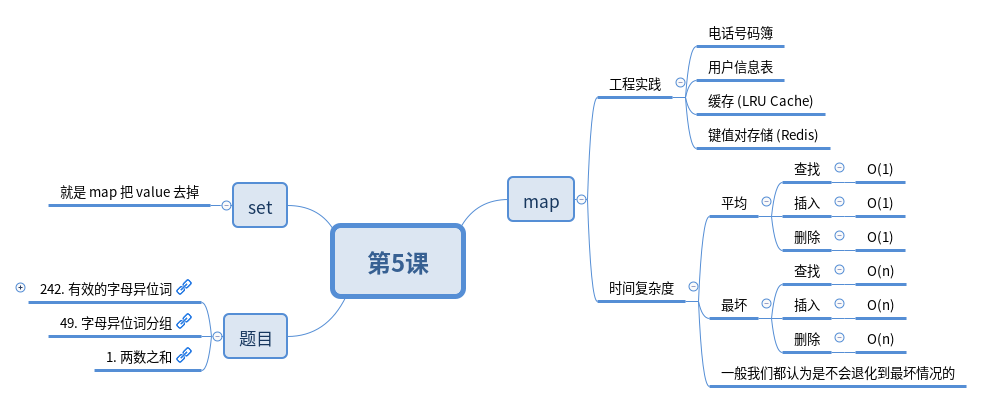
\includegraphics[width=170mm,height=80mm]{images/camp/第5课.png}

\subsubsection{题目}

\begin{itemize}
\item \hyperref[leetcode:242]{242. 有效的字母异位词}
\item \hyperref[leetcode:49]{49. 字母异位词分组}
\item \hyperref[leetcode:1]{1. 两数之和}
\end{itemize}

\subsection{第 6 课 | 树、二叉树、二叉搜索树}

\subsubsection{脑图}

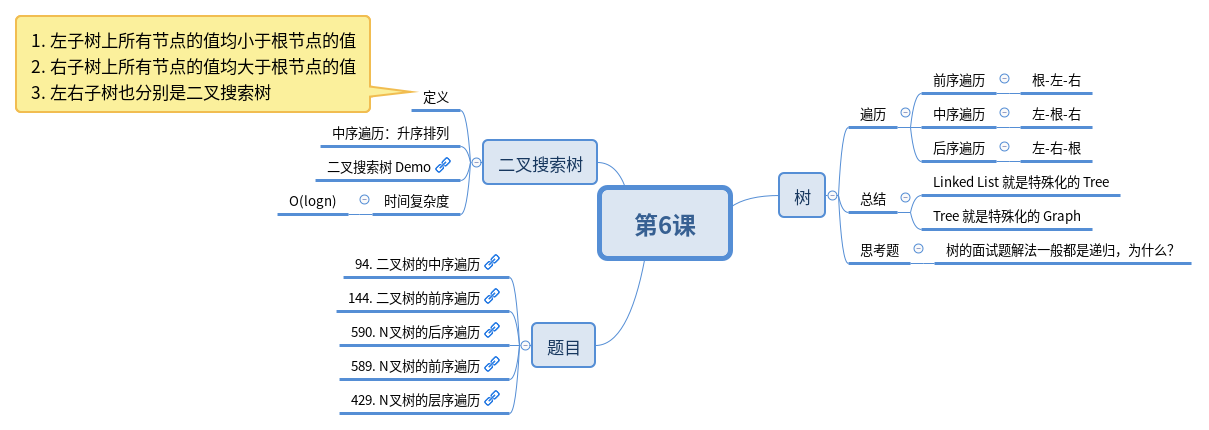
\includegraphics[width=170mm,height=80mm]{images/camp/第6课.png}

\subsubsection{题目}

\begin{itemize}
  \item \hyperref[leetcode:94]{94. 二叉树的中序遍历}
  \item \hyperref[leetcode:144]{144. 二叉树的前序遍历}
  \item \hyperref[leetcode:590]{590. N叉树的后序遍历}
  \item \hyperref[leetcode:589]{589. N叉树的前序遍历}
  \item \hyperref[leetcode:429]{429. N叉树的层序遍历}
\end{itemize}

\newpage
\section{第 7 课}

\subsection{脑图}

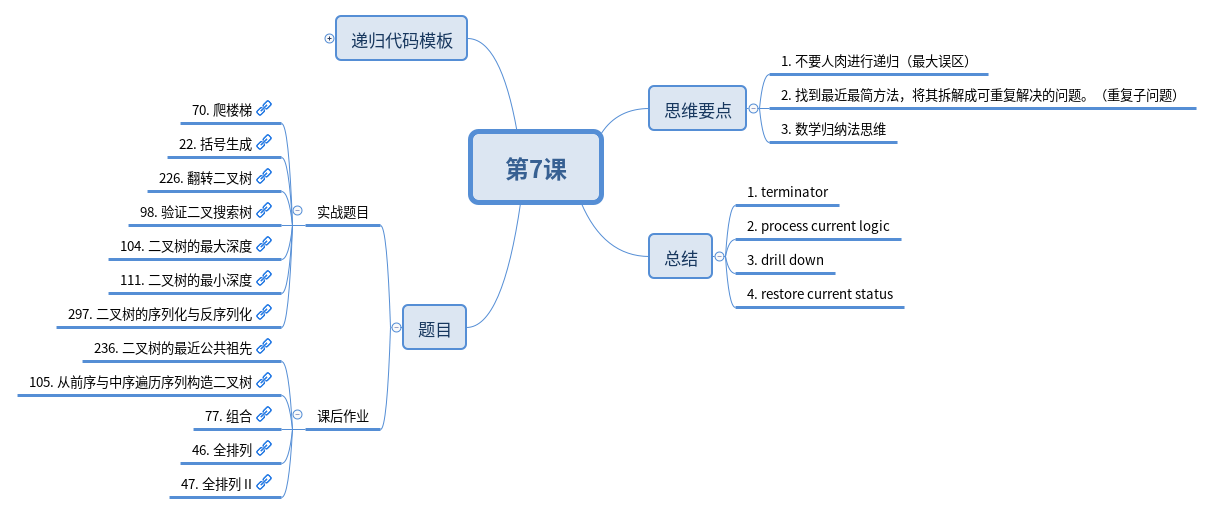
\includegraphics[width=170mm,height=80mm]{images/第7课.png}

\subsection{题目}

\subsubsection{实战题目}

\begin{itemize}
  \item \hyperref[leetcode:70]{70. 爬楼梯}
  \item \hyperref[leetcode:22]{22. 括号生成}
  \item \hyperref[leetcode:226]{226. 翻转二叉树}
  \item \hyperref[leetcode:98]{98. 验证二叉搜索树}
  \item \hyperref[leetcode:104]{104. 二叉树的最大深度}
  \item \hyperref[leetcode:111]{111. 二叉树的最小深度}
  \item \hyperref[leetcode:297]{297. 二叉树的序列化与反序列化}
\end{itemize}

\subsubsection{课后作业}

\begin{itemize}
  \item \hyperref[leetcode:236]{236. 二叉树的最近公共祖先}
  \item \hyperref[leetcode:105]{105. 从前序与中序遍历序列构造二叉树}
  \item \hyperref[leetcode:77]{77. 组合}
  \item \hyperref[leetcode:46]{46. 全排列}
  \item \hyperref[leetcode:47]{47. 全排列 II}
\end{itemize}


\subsection{学习总结}

这周学习了哈希表、集合、树、递归。

哈希表的平均时间复杂度都是 O(1) 的,所以在工程实践中被广泛使用。
大部分的语言里面都是有内置的哈希表。哈希表的最坏时间复杂度虽然
是 O(n) 的,但是一般都会设计为可自动扩容,所以一般我们都认为是
不会退化到最坏的情况的。

链表就是特殊化的树。\\
树就是特殊化的图。\\
树需要掌握前序遍历、中序遍历、后序遍历。\\
二叉搜索树的中序遍历得到的结果是有序的。\\
树这个数据结构的定义就是递归定义的,具有重复子问题,
非常适合使用递归解决树的相关问题。

递归模板:
\begin{verbatim}
// terminator
// process current logic
// drill down
// restore current status
\end{verbatim}

\newpage
\section{第 03 周}

\subsection{第 8 课 | 分治、回溯}

\subsubsection{脑图}

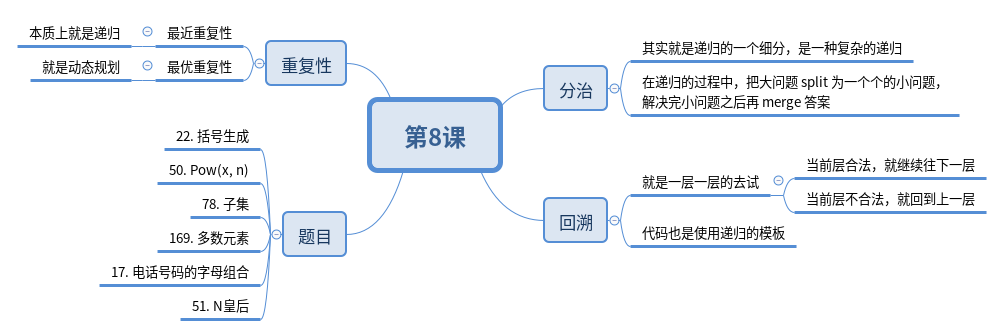
\includegraphics[width=170mm,height=80mm]{images/camp/第8课.png}

\subsubsection{题目}

\begin{itemize}
  \item \hyperref[leetcode:22]{22. 括号生成}
  \item \hyperref[leetcode:50]{50. Pow(x, n)}
  \item \hyperref[leetcode:78]{78. 子集}
  \item \hyperref[leetcode:169]{169. 多数元素}
  \item \hyperref[leetcode:17]{17. 电话号码的字母组合}
  \item \hyperref[leetcode:51]{51. N皇后}
\end{itemize}

\subsection{第 9 课 | DFS 和 BFS}

\subsubsection{脑图}

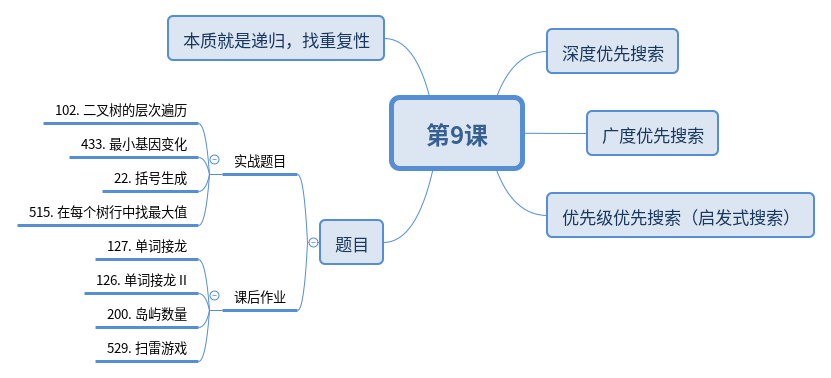
\includegraphics[width=170mm,height=80mm]{images/camp/第9课.png}

\subsubsection{题目}

\paragraph{实战题目}

\begin{itemize}
  \item \hyperref[leetcode:102]{102. 二叉树的层次遍历}
  \item \hyperref[leetcode:433]{433. 最小基因变化}
  \item \hyperref[leetcode:22]{22. 括号生成}
  \item \hyperref[leetcode:515]{515. 在每个树行中找最大值}
\end{itemize}

\paragraph{课后作业}

\begin{itemize}
  \item \hyperref[leetcode:127]{127. 单词接龙}
  \item \hyperref[leetcode:126]{126. 单词接龙 II}
  \item \hyperref[leetcode:200]{200. 岛屿数量}
  \item \hyperref[leetcode:529]{529. 扫雷游戏}
\end{itemize}

\subsection{第 10 课 | 贪心算法}

\subsubsection{脑图}

\subsubsection{题目}

\subsection{第 11 课 | 二分查找}

\subsubsection{脑图}

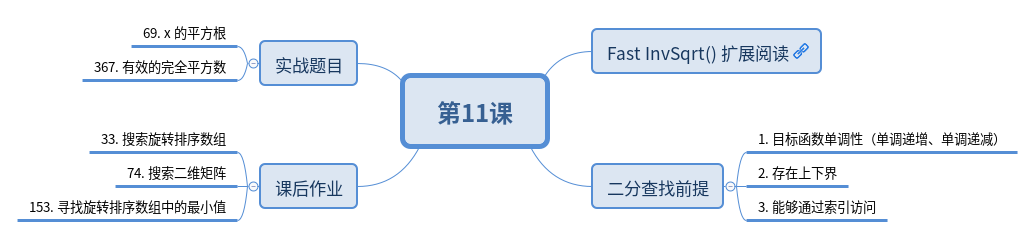
\includegraphics[width=170mm,height=80mm]{images/第11课.png}

\subsubsection{题目}

\paragraph{实战题目}

\begin{itemize}
  \item \hyperref[leetcode:69]{69. x 的平方根}
  \item \hyperref[leetcode:367]{367. 有效的完全平方数}
\end{itemize}

\paragraph{课后作业}

\begin{itemize}
  \item \hyperref[leetcode:33]{33. 搜索旋转排序数组}
  \item \hyperref[leetcode:74]{74. 搜索二维矩阵}
  \item \hyperref[leetcode:153]{153. 寻找旋转排序数组中的最小值}
  \item 使用二分查找,寻找一个半有序数组 [4, 5, 6, 7, 0, 1, 2] 中间无序的地方
    说明:同学们可以将自己的思路、代码写在第 3 周的学习总结中
\end{itemize}


\subsection{学习总结}

\newpage
\section{第 05 周}

\subsection{第 12 课 | 动态规划}

\subsubsection{脑图}

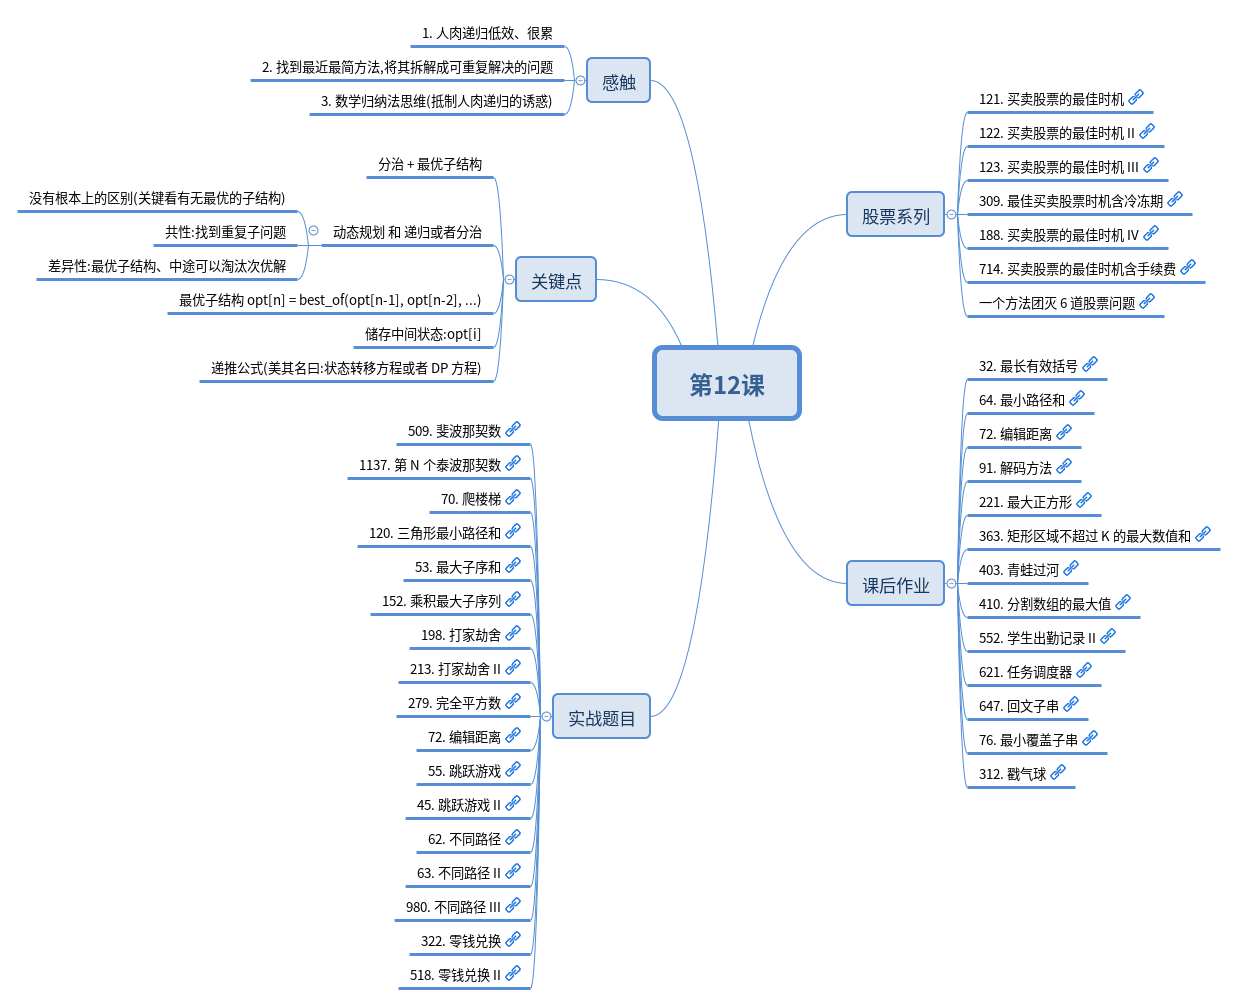
\includegraphics[width=170mm,height=160mm]{images/camp/第12课.png}

\subsubsection{题目}

\paragraph{实战题目}

\begin{itemize}
  \item \hyperref[leetcode:509]{509. 斐波那契数}
  \item \hyperref[leetcode:1137]{1137. 第 N 个泰波那契数}
  \item \hyperref[leetcode:70]{70. 爬楼梯}
  \item \hyperref[leetcode:120]{120. 三角形最小路径和}
  \item \hyperref[leetcode:53]{53. 最大子序和}
  \item \hyperref[leetcode:152]{152. 乘积最大子序列}
  \item \hyperref[leetcode:198]{198. 打家劫舍}
  \item \hyperref[leetcode:213]{213. 打家劫舍 II}
\end{itemize}

\paragraph{高级 DP 实战题目}

\begin{itemize}
  \item \hyperref[leetcode:279]{279. 完全平方数}
  \item \hyperref[leetcode:72]{72. 编辑距离}
  \item \hyperref[leetcode:55]{55. 跳跃游戏}
  \item \hyperref[leetcode:45]{45. 跳跃游戏 II}
  \item \hyperref[leetcode:62]{62. 不同路径}
  \item \hyperref[leetcode:63]{63. 不同路径 II}
  \item \hyperref[leetcode:980]{980. 不同路径 III}
  \item \hyperref[leetcode:322]{322. 零钱兑换}
  \item \hyperref[leetcode:518]{518. 零钱兑换 II}
\end{itemize}

\paragraph{股票系列题目}

\begin{itemize}
  \item \hyperref[leetcode:121]{121. 买卖股票的最佳时机}
  \item \hyperref[leetcode:122]{122. 买卖股票的最佳时机 II}
  \item \hyperref[leetcode:123]{123. 买卖股票的最佳时机 III}
  \item \hyperref[leetcode:309]{309. 最佳买卖股票时机含冷冻期}
  \item \hyperref[leetcode:188]{188. 买卖股票的最佳时机 IV}
  \item \hyperref[leetcode:714]{714. 买卖股票的最佳时机含手续费}
  \item \href{https://leetcode-cn.com/problems/best-time-to-buy-and-sell-stock/solution/yi-ge-fang-fa-tuan-mie-6-dao-gu-piao-wen-ti-by-l-3/}{一个方法团灭 6 道股票问题}
\end{itemize}

\paragraph{课后作业}

\begin{itemize}
  \item \hyperref[leetcode:32]{32. 最长有效括号}
  \item \hyperref[leetcode:64]{64. 最小路径和}
  \item \hyperref[leetcode:72]{72. 编辑距离}
  \item \hyperref[leetcode:91]{91. 解码方法}
  \item \hyperref[leetcode:221]{221. 最大正方形}
  \item \hyperref[leetcode:363]{363. 矩形区域不超过 K 的最大数值和}
  \item \hyperref[leetcode:403]{403. 青蛙过河}
  \item \hyperref[leetcode:410]{410. 分割数组的最大值}
  \item \hyperref[leetcode:552]{552. 学生出勤记录 II}
  \item \hyperref[leetcode:621]{621. 任务调度器}
  \item \hyperref[leetcode:647]{647. 回文子串}
  \item \hyperref[leetcode:76]{76. 最小覆盖子串}
  \item \hyperref[leetcode:312]{312. 戳气球}
\end{itemize}


\subsection{学习总结}

这周学习了动态规划,这个还是挺难的。

动态规划关键点:

\begin{itemize}
  \item 最优子结构 opt[n] = best\_of(opt[n-1], opt[n-2], ...)
  \item 储存中间状态:opt[i]
  \item 递推公式(美其名曰:状态转移方程或者 DP 方程)
\end{itemize}

感觉还是需要把基础的题目多刷几遍之后,才会更有感觉吧。
不然总觉得换个题目了就又不会了。


\chapter{代码模板}

\newpage
\section{递归模板}

\begin{enumerate}
  \item // terminator
  \item // process current logic
  \item // drill down
  \item // restore current status
\end{enumerate}

\subsection{Python 递归模板}

\begin{verbatim}
def recursion(level, param1, param2, ...):
  # recursion terminator
  if level > MAX_LEVEL:
    print_result
    return

  # process logic in current level
  process_data(level, data, ...)

  # drill down
  self.recursion(level + 1, p1, p2, ...)

  # reverse the current level status if needed
  reverse_state(level)
\end{verbatim}
\newpage
\section{DFS 深度优先遍历模板}

\subsection{Python DFS 模板,递归写法}

\begin{verbatim}
visited = set()
def dfs(node, visited):
  if node in visited: # terminator
    # already visited
    return
  
  visited.add(node)

  # process current node here
  ...

  for next_node in node.children():
    if next_node not in visited:
      dfs(next_node, visited)
\end{verbatim}

\subsection{Python DFS 模板,非递归写法}

\begin{verbatim}
def DFS(self, tree):
  if tree.root is None:
    return []

  visited, stack = [], [tree.root]

  while stack:
    node = stack.pop()
    visited.add(node)

    process (node)
    nodes = generate_related_nodes(node)
    stack.push(nodes)
  
  # other processing work
  ...
\end{verbatim}

\newpage
\section{BFS 广度优先遍历模板}

\subsection{Python BFS 模板}

\begin{verbatim}
def BFS(graph, start, end):
  visited = set()
  queue = []
  queue.append([start])

  while queue:
    node = queue.pop()
    visited.add(node)

    process(node)
    nodes = generate_related_nodes(node)
    queue.push(nodes)

  # other processing work
\end{verbatim}

\newpage
\section{二分查找模板}

\subsection{Python 二分查找模板}

\begin{verbatim}
def binarySearch(array, target):
  left, right = 0, len(array) - 1
  while left <= right:
    mid = left + (right - left) / 2
    if array[mid] == target:
      break or return result
    elif array[mid] < target:
      left = mid + 1
    else:
      right = mid - 1
\end{verbatim}
\newpage
\section{分治模板}

\subsection{Python 分治模板}

\begin{verbatim}
def divide_conquer(problem, param1, param2, ...): 
  # recursion terminator 
  if problem is None: 
    print_result 
    return 

  # prepare data 
  data = prepare_data(problem) 
  subproblems = split_problem(problem, data) 

  # conquer subproblems 
  subresult1 = self.divide_conquer(subproblems[0], p1, ...) 
  subresult2 = self.divide_conquer(subproblems[1], p1, ...) 
  subresult3 = self.divide_conquer(subproblems[2], p1, ...) 
  …

  # process and generate the final result 
  result = process_result(subresult1, subresult2, subresult3, …)
	
  # revert the current level states
\end{verbatim}

\newpage
\section{树的前中后序遍历}

\subsection{Python 遍历模板}

\begin{verbatim}
def preorder(self, root):
  if root:
    self.traverse_path.append(root.val)
    self.preorder(root.left)
    self.preorder(root.right)

def inorder(self, root):
  if root:
    self.inorder(root.left)
    self.traverse_path.append(root.val)
    self.inorder(root.right)

def postorder(self, root):
  if root:
    self.postorder(root.left)
    self.postorder(root.right)
    self.traverse_path.append(root.val)
\end{verbatim}

\newpage
\section{字典树}

\subsection{Python 模板}

\begin{verbatim}
class Trie(object):
  def __init__(self):
    self.root = {}
    self.end_of_word = "#"

  def insert(self, word):
    node = self.root
    for char in word:
      node = node.setdefault(char, {})
    node[self.end_of_word] = self.end_of_word

  def search(self, word):
    node = self.root
    for char in word:
      if char not in node:
        return False
      node = node[char]
    return self.end_of_word in node

  def startsWith(self, prefix):
    node = self.root
    for char in prefix:
      if char not in node:
        return False
      node = node[char]
    return True
\end{verbatim}

\newpage
\section{并查集}

\subsection{Java 模板}

\begin{verbatim}
class UnionFind {
  private int count = 0;
  private int[] parent;
  public UnionFind(int n) {
    count = n;
    parent = new int[n];
    for (int i = 0; i < n; i++) {
      parent[i] = i;
    }
  }
  public int find(int p) {
    while (p != parent[p]) {
      parent[p] = parent[parent[p]];
      p = parent[p];
    }
    return p;
  }
  public void union(int p, int q) {
    int rootP = find(p);
    int rootQ = find(q);
    if (rootP == rootQ) return;
    parent[rootP] = rootQ;
    count--;
  }
}
\end{verbatim}

\subsection{Python 模板}

\begin{verbatim}
def init(p):
  # for i = 0 .. n: p[i] = i;
  p = [i for i in range(n)]

def union(self, p, i, j):
  p1 = self.parent(p, i)
  p2 = self.parent(p, j)
  p[p1] = p2

def parent(self, p, i):
  root = i
  while p[root] != root:
    root = p[root]
  while p[i] != i: # 路径压缩 ?
    x = i; i = p[i]; p[x] = root
  return root
\end{verbatim}

\newpage
\section{布隆过滤器模板}

\subsection{Python 模板}

\begin{verbatim}
from bitarray import bitarray
import mmh3

class BloomFilter:
  def __init__(self, size, hash_num):
    self.size = size
    self.hash_num = hash_num
    self.bit_array = bitarray(size)
    self.bit_array.setall(0)

  def add(self, s):
    for seed in range(self.hash_num):
      result = mmh3.hash(s, seed) % self.size
      self.bit_array[result] = 1

  def lookup(self, s):
    for seed in range(self.hash_num):
      result = mmh3.hash(s, seed) % self.size
      if self.bit_array[result] == 0:
        return "Nope"
    return "Probably"

bf = BloomFilter(500000, 7)
bf.add("dantezhao")
print (bf.lookup("dantezhao"))
print (bf.lookup("yyj"))
\end{verbatim}

\newpage
\section{LRU cache 模板}

\subsection{Python 模板}

\begin{verbatim}
class LRUCache(object):

def __init__(self, capacity):
  self.dic = collections.OrderedDict()
  self.remain = capacity

def get(self, key):
  if key not in self.dic:
    return -1
  v = self.dic.pop(key)
  self.dic[key] = v   # key as the newest one
  return v

def put(self, key, value):
  if key in self.dic:
    self.dic.pop(key)
  else:
    if self.remain > 0:
      self.remain -= 1
    else:   # self.dic is full
      self.dic.popitem(last=False)
  self.dic[key] = value
\end{verbatim}

\subsection{Java 模板}

\begin{verbatim}
public class LRUCache {
  private Map<Integer, Integer> map;
  public LRUCache(int capacity) {
    map = new LinkedCappedHashMap<>(capacity);
  }
  public int get(int key) {
    if(!map.containsKey(key)) { return -1; }
    return map.get(key);
  }
  public void put(int key, int value) {
    map.put(key,value);
  }
  private static class LinkedCappedHashMap<K,V> extends LinkedHashMap<K,V> {
    int maximumCapacity;
    LinkedCappedHashMap(int maximumCapacity) {
      super(16, 0.75f, true);
      this.maximumCapacity = maximumCapacity;
    }
    protected boolean removeEldestEntry(Map.Entry eldest) {
      return size() > maximumCapacity;
    }
  }
}
\end{verbatim}

\newpage
\section{快速排序模板}

\subsection{JavaScript 模板}

\begin{verbatim}
function QuickSort(a, start = 0, end = a.length - 1) {
  if (start < end) {
    const partitionIndex = partition(a, start, end);
    QuickSort(a, start, partitionIndex - 1);
    QuickSort(a, partitionIndex + 1, end);
  }
}

function partition(a, start, end) {
  const pivot = a[end];
  let partitionIndex = start;
  for (let i = start; i < end; i += 1) {
    if (a[i] < pivot) {
      swap(a, partitionIndex, i);
      partitionIndex += 1;
    }
  }
  swap(a, partitionIndex, end);
  return partitionIndex;
}

function swap(a, i, j) {
  const temp = a[i];
  a[i] = a[j];
  a[j] = temp;
}
\end{verbatim}

\subsection{Python 模板}

\begin{verbatim}
def QuickSort(a):
  quickSort(a, 0, len(a) - 1)

def quickSort(a, start, end):
  if start < end:
    partitionIndex = partition(a, start, end)
    quickSort(a, start, partitionIndex - 1)
    quickSort(a, partitionIndex + 1, end)

def partition(a, start, end):
  pivot = a[end]
  partitionIndex = start
  for i in range(start, end):
    if a[i] < pivot:
      a[i], a[partitionIndex] = a[partitionIndex], a[i]
      partitionIndex += 1
  a[partitionIndex], a[end] = a[end], a[partitionIndex]
  return partitionIndex
\end{verbatim}

\subsection{Java 模板}

\begin{verbatim}
public static void quickSort(int[] array, int begin, int end) {
  if (end <= begin) return;
  int pivot = partition(array, begin, end);
  quickSort(array, begin, pivot - 1);
  quickSort(array, pivot + 1, end);
}

static int partition(int[] a, int begin, int end) {
  // pivot: 标杆位置,counter: 小于pivot的元素的个数
  int pivot = end, counter = begin;
  for (int i = begin; i < end; i++) {
    if (a[i] < a[pivot]) {
      int temp = a[counter]; a[counter] = a[i]; a[i] = temp;
      counter++;
    }
  }
  int temp = a[pivot]; a[pivot] = a[counter]; a[counter] = temp;
  return counter;
}
\end{verbatim}

\newpage
\section{归并排序模板}

\subsection{JavaScript 模板}

\begin{verbatim}
function MergeSort(array, left, right) {
  if (right <= left) { return; }
  const mid = Math.floor((left + right) / 2);
  MergeSort(array, left, mid);
  MergeSort(array, mid+1, right);
  merge(array, left, mid, right);
}

function merge(array, left, mid, right) {
  const temp = new Array(right - left + 1);
  [i, j, k] = [left, mid+1, 0]
  while (i <= mid && j <= right) {
    temp[k++] = array[i] <= array[j] ? array[i++] : array[j++];
  }
  while (i <= mid) {
    temp[k++] = array[i++];
  }
  while (j <= right) {
    temp[k++] = array[j++];
  }
  for (let p = 0; p < temp.length; p += 1) {
    array[left + p] = temp[p];
  }
}
\end{verbatim}

\subsection{Java 模板}

\begin{verbatim}
public static void mergeSort(int[] array, int left, int right) {
  if (right <= left) return;
  int mid = (left + right) >> 1; // (left + right) / 2

  mergeSort(array, left, mid);
  mergeSort(array, mid + 1, right);
  merge(array, left, mid, right);
}

public static void merge(int[] arr, int left, int mid, int right) {
  int[] temp = new int[right - left + 1]; // 中间数组
  int i = left, j = mid + 1, k = 0;

  while (i <= mid && j <= right) {
    temp[k++] = arr[i] <= arr[j] ? arr[i++] : arr[j++];
  }

  while (i <= mid)   temp[k++] = arr[i++];
  while (j <= right) temp[k++] = arr[j++];

  for (int p = 0; p < temp.length; p++) {
    arr[left + p] = temp[p];
  }
  // 也可以用 System.arraycopy(a, start1, b, start2, length)
}
\end{verbatim}

\newpage
\section{堆排序模板}

\subsection{Python 模板}

\begin{verbatim}
import heapq
class Solution:
  def sortArray(self, nums: List[int]) -> List[int]:
    heapq.heapify(nums)
    return [heapq.heappop(nums) for _ in range(len(nums))]
\end{verbatim}

\subsection{C++ 模板}

\begin{verbatim}
void heap_sort(int a[], int len) {
  priority_queue<int,vector<int>,greater<int> > q;
  for(int i = 0; i < len; i++) {
    q.push(a[i]);
  }
  for(int i = 0; i < len; i++) {
    a[i] = q.pop();
  }
}
\end{verbatim}

\subsection{Java 模板}

\begin{verbatim}
static void heapify(int[] array, int length, int i) {
  int left = 2 * i + 1, right = 2 * i + 2;
  int largest = i;

  if (left < length && array[left] > array[largest]) {
    largest = left;
  }
  if (right < length && array[right] > array[largest]) {
    largest = right;
  }

  if (largest != i) {
    int temp = array[i]; array[i] = array[largest]; array[largest] = temp;
    heapify(array, length, largest);
  }
}

public static void heapSort(int[] array) {
  if (array.length == 0) return;

  int length = array.length;
  for (int i = length / 2-1; i >= 0; i-)
    heapify(array, length, i);

  for (int i = length - 1; i >= 0; i--) {
    int temp = array[0]; array[0] = array[i]; array[i] = temp;
    heapify(array, i, 0);
  }
}
\end{verbatim}

\newpage
\section{Atoi 字符串转整数模板}

\subsection{Java 模板}

\begin{verbatim}
public int myAtoi(String str) {
  int index = 0, sign = 1, total = 0;
  //1. Empty string
  if(str.length() == 0) return 0;

  //2. Remove Spaces
  while(str.charAt(index) == ' ' && index < str.length())
    index ++;

  //3. Handle signs
  if(str.charAt(index) == '+' || str.charAt(index) == '-'){
    sign = str.charAt(index) == '+' ? 1 : -1;
    index ++;
  }

  //4. Convert number and avoid overflow
  while(index < str.length()){
    int digit = str.charAt(index) - '0';
    if(digit < 0 || digit > 9) break;

    //check if total will be overflow after 10 times and add digit
    if(Integer.MAX_VALUE/10 < total ||
      Integer.MAX_VALUE/10 == total && Integer.MAX_VALUE %10 < digit)
      return sign == 1 ? Integer.MAX_VALUE : Integer.MIN_VALUE;

    total = 10 * total + digit;
    index ++;
  }
  return total * sign;
}
\end{verbatim}

\subsection{Python 模板}

\begin{verbatim}
class Solution(object):
  def myAtoi(self, s):
    if len(s) == 0 : return 0
    ls = list(s.strip())

    sign = -1 if ls[0] == '-' else 1

    if ls[0] in ['-','+'] : del ls[0]

    ret, i = 0, 0

    while i < len(ls) and ls[i].isdigit() :
      ret = ret*10 + ord(ls[i]) - ord('0')
      i += 1

    return max(-2**31, min(sign * ret,2**31-1))
\end{verbatim}

\newpage
\section{字符串匹配暴力法模板}

\subsection{Java 模板}

\begin{verbatim}
public static int forceSearch(String txt, String pat) {
  int M = txt.length();
  int N = pat.length();

  for (int i = 0; i <= M - N; i++) {
    int j;
    for (j = 0; j < N; j++) {
      if (txt.charAt(i + j) != pat.charAt(j))
        break;
    }
    if (j == N) {
      return i;
    }
    // 更加聪明?
    // 1. 预先判断 hash(txt.substring(i, M)) == hash(pat)
    // 2. KMP
  }
  return -1;
}
\end{verbatim}

\newpage
\section{字符串Rabin-Karp模板}

\subsection{Java 模板}

\begin{verbatim}
public final static int D = 256;
public final static int Q = 9997;

static int RabinKarpSerach(String txt, String pat) {
  int M = pat.length();
  int N = txt.length();
  int i, j;
  int patHash = 0, txtHash = 0;

  for (i = 0; i < M; i++) {
    patHash = (D * patHash + pat.charAt(i)) % Q;
    txtHash = (D * txtHash + txt.charAt(i)) % Q;
  }

  int highestPow = 1;  // pow(256, M-1)
  for (i = 0; i < M - 1; i++)
    highestPow = (highestPow * D) % Q;

  for (i = 0; i <= N - M; i++) { // 枚举起点
    if (patHash == txtHash) {
      for (j = 0; j < M; j++) {
        if (txt.charAt(i + j) != pat.charAt(j))
          break;
      }
      if (j == M)
        return i;
    }
    if (i < N - M) {
      txtHash = (D * (txtHash - txt.charAt(i) * highestPow) + txt.charAt(i + M)) % Q;
      if (txtHash < 0)
        txtHash += Q;
    }
  }

  return -1;
}
\end{verbatim}


\chapter{LeetCode 专题}

\newpage
\section{跳跃游戏}

\begin{itemize}
  \item \hyperref[leetcode:55]{55. 跳跃游戏}
  \item \hyperref[leetcode:45]{45. 跳跃游戏 II}
  \item \hyperref[leetcode:1306]{1306. 跳跃游戏 III}
  \item \hyperref[leetcode:1345]{1345. 跳跃游戏 IV}
  \item \hyperref[leetcode:1340]{1340. 跳跃游戏 V}
  \item \hyperref[leetcode:lcp_09]{LCP 09. 最小跳跃次数}
\end{itemize}



\chapter{LeetCode 题目(1-200)}

\newpage
\section{1. 两数之和}
\label{leetcode:1}

\subsection{题目}

给定一个整数数组 nums 和一个目标值 target,
请你在该数组中找出和为目标值的那\textbf{两个}整数,并返回他们的数组下标。

你可以假设每种输入只会对应一个答案。但是,你不能重复利用这个数组中同样的元素。

\textbf{示例}:

\begin{verbatim}
  给定 nums = [2, 7, 11, 15], target = 9

  因为 nums[0] + nums[1] = 2 + 7 = 9
  所以返回 [0, 1]
\end{verbatim}

\subsection{参考题解,暴力法}

直接两重循环,遍历两个数的所有组合情况。
因为两重循环,所以时间复杂度为 O(n$^{2}$)。
因为没有而外开辟空间,所以空间复杂度为 O(1)。

\begin{verbatim}
/**
 * @param {number[]} nums
 * @param {number} target
 * @return {number[]}
 */
var twoSum = function(nums, target) {
  for (let i = 0; i < nums.length; i += 1) {
    for (let j = i + 1; j < nums.length; j += 1) {
      if (nums[i] + nums[j] === target) {
        return [i, j];
      }
    }
  }
};
\end{verbatim}

\subsection{参考题解,哈希表,两重循环}

因为 numA + numB = target,所以 numA = target - numB。
那我们可以考虑把 numA 的所有可能保存到哈希表,
然后第二次循环 numB 的时候,直接在哈希表中查找。

时间复杂度: O(n)。\\
空间复杂度: O(n)。

\begin{verbatim}
/**
 * @param {number[]} nums
 * @param {number} target
 * @return {number[]}
 */
var twoSum = function(nums, target) {
  const m = new Map();
  for (let i = 0; i < nums.length; i += 1) {
    m.set(nums[i], i);
  }
  for (let i = 0; i < nums.length; i += 1) {
    const num = nums[i];
    const peer = target - num;
    if (m.has(peer) && m.get(peer) !== i) {
      return [i, m.get(peer)];
    }
  }
};
\end{verbatim}

\subsection{参考题解,哈希表,一重循环}

这种方法是在上一种的基础上再次优化,减少了一重循环,
不过时间复杂度和空间复杂度还是一样的。

时间复杂度: O(n)。\\
空间复杂度: O(n)。

\begin{verbatim}
/**
 * @param {number[]} nums
 * @param {number} target
 * @return {number[]}
 */
var twoSum = function(nums, target) {
  const m = new Map();
  for (let i = 0; i < nums.length; i += 1) {
    const num = nums[i];
    const peer = target - num;
    if (m.has(peer)) {
      return [m.get(peer), i];
    }
    m.set(num, i);
  }
};
\end{verbatim}

\subsection{题目小结}

通过上面 3 种题解,你会发现这就是非常明显的空间换时间。
在工程项目中也是非常常用的方法,所以要熟练掌握哈希表。

\subsection{题目拓展}

如果题目要求返回的不是下标,而是两个整数的值,
那你还有其他方法吗?

答案是\textbf{双指针两头夹逼}的方法。该方法要求数组是有序的,
所以需要先对数组进行排序。如果是要返回下标的话,排序了
之后,下标就改变了,就不适合用\textbf{双指针两头夹逼}的方法。

下面给出如果是返回整数的值的参考代码:

\begin{verbatim}
var twoSum = function(nums, target) {
  nums.sort((a, b) => a - b);
  let [start, end] = [0, nums.length - 1];
  while (start < end) {
    const sum = nums[start] + nums[end];
    if (sum < target) {
      start += 1;
    } else if (sum > target) {
      end -= 1;
    } else {
      return [nums[start], nums[end]];
    }
  }
};
\end{verbatim}

\newpage
\section{5. 最长回文子串}
\label{leetcode:5}

\subsection{题目}

给定一个字符串 s,找到 s 中最长的回文子串。你可以假设 s 的最大长度为 1000。

\textbf{示例 1}:

\begin{verbatim}
  输入: "babad"
  输出: "bab"
  注意: "aba" 也是一个有效答案。
\end{verbatim}

\textbf{示例 2}:

\begin{verbatim}
  输入: "cbbd"
  输出: "bb"
\end{verbatim}

\subsection{参考题解}

\subsubsection{Python}

\begin{verbatim}
class Solution:
  # dp[i][j]
  # i 表示字符串的起点
  # j 表示字符串的终点
  #
  # dp[i][j] = true 表示 s[i, j] 是回文串
  # dp[i][j] = false 表示 s[i, j] 不是回文串
  #
  # dp[i][j] = (dp[i+1][j-1] && s[i] == s[j])
  # 因为 s[i+1, j-1] 是回文串,且 s[i] == s[j]
  # 所以向左右两边扩展一个字母,则
  # dp[i][j] 也是回文串
  def longestPalindrome(self, s: str) -> str:
    n, result = len(s), ""
    dp = [[False for _ in range(n)] for _ in range(n)]
    for i in range(n - 1, -1, -1):
      for j in range(i, n):
        dp[i][j] = s[i] == s[j] and (j - i < 2 or dp[i + 1][j - 1])
        if dp[i][j] and j - i + 1 > len(result):
          result = s[i:j + 1]
    return result
\end{verbatim}


\newpage
\section{8. 字符串转换整数 (atoi)}
\label{leetcode:8}

\subsection{题目}

请你来实现一个 atoi 函数,使其能将字符串转换成整数。

首先,该函数会根据需要丢弃无用的开头空格字符,直到寻找到第一个非空格的字符为止。

当我们寻找到的第一个非空字符为正或者负号时,则将该符号与之后面尽可能多的连续数字组合起来,
作为该整数的正负号;假如第一个非空字符是数字,则直接将其与之后连续的数字字符组合起来,形成整数。

该字符串除了有效的整数部分之后也可能会存在多余的字符,这些字符可以被忽略,它们对于函数不应该造成影响。

注意:假如该字符串中的第一个非空格字符不是一个有效整数字符、字符串为空或字符串仅包含空白字符时,
则你的函数不需要进行转换。

在任何情况下,若函数不能进行有效的转换时,请返回 0。

\textbf{说明}:

假设我们的环境只能存储 32 位大小的有符号整数,那么其数值范围为 [−$2^{31}$,  $2^{31}$ − 1]。
如果数值超过这个范围,请返回  INT\_MAX ($2^{31}$ − 1) 或 INT\_MIN (−$2^{31}$) 。

\textbf{示例 1}:

\begin{verbatim}
  输入: "42"
  输出: 42
\end{verbatim}

\textbf{示例 2}:

\begin{verbatim}
  输入: "   -42"
  输出: -42
  解释: 第一个非空白字符为 '-', 它是一个负号。
       我们尽可能将负号与后面所有连续出现的数字组合起来,最后得到 -42 。
\end{verbatim}

\textbf{示例 3}:

\begin{verbatim}
  输入: "4193 with words"
  输出: 4193
  解释: 转换截止于数字 '3' ,因为它的下一个字符不为数字。
\end{verbatim}

\textbf{示例 4}:

\begin{verbatim}
  输入: "words and 987"
  输出: 0
  解释: 第一个非空字符是 'w', 但它不是数字或正、负号。
      因此无法执行有效的转换。
\end{verbatim}

\textbf{示例 5}:

\begin{verbatim}
  输入: "-91283472332"
  输出: -2147483648
  解释: 数字 "-91283472332" 超过 32 位有符号整数范围。
       因此返回 INT_MIN (−2^31) 。
\end{verbatim}

\subsection{参考题解}

\subsubsection{Python}

\begin{verbatim}
class Solution:
  def myAtoi(self, s: str) -> int:
    if len(s) == 0: return 0
    ls = list(s.strip())
    if len(ls) == 0: return 0
    sign = -1 if ls[0] == '-' else 1
    if ls[0] in ['-', '+']: del ls[0]
    ret, i = 0, 0
    while i < len(ls) and ls[i].isdigit():
      ret = ret * 10 + ord(ls[i]) - ord('0')
      i += 1
    return max(-2**31, min(sign * ret, 2**31 - 1))
\end{verbatim}

\newpage
\section{10. 正则表达式匹配}
\label{leetcode:10}

\subsection{题目}

\newpage
\section{11. 盛最多水的容器}
\label{leetcode:11}

\begin{verbatim}
/**
 * @param {number[]} height
 * @return {number}
 */
var maxArea = function(height) {
  let result = 0;
  let left = 0;
  let right = height.length - 1;
  while (left < right) {
    let curWidth = right - left;
    let curHeight = Math.min(height[left], height[right]);
    let curArea = curWidth * curHeight;
    if (curArea > result) {
      result = curArea;
    }

    if (height[left] < height[right]) {
      left += 1;
    } else {
      right -= 1;
    }
  }
  return result;
};
\end{verbatim}

\newpage
\section{14. 最长公共前缀}
\label{leetcode:14}

\subsection{题目}

编写一个函数来查找字符串数组中的最长公共前缀。

如果不存在公共前缀,返回空字符串 \verb|""|。

\textbf{示例 1}:

\begin{verbatim}
  输入: ["flower","flow","flight"]
  输出: "fl"
\end{verbatim}

\textbf{示例 2}:

\begin{verbatim}
  输入: ["dog","racecar","car"]
  输出: ""
  解释: 输入不存在公共前缀。
\end{verbatim}

\textbf{说明}:

所有输入只包含小写字母 a-z 。

\subsection{参考题解}

\subsubsection{Python}

\begin{verbatim}
class Solution:
  def longestCommonPrefix(self, strs: List[str]) -> str:
    if len(strs) == 0: return ""
    for i in range(len(strs[0])):
      c = strs[0][i]
      for j in range(1, len(strs)):
        if i == len(strs[j]) or c != strs[j][i]:
          return strs[0][:i]
    return strs[0]
\end{verbatim}

\newpage
\section{15. 三数之和}
\label{leetcode:15}

\begin{verbatim}
/**
 * @param {number[]} nums
 * @return {number[][]}
 */
var threeSum = function(nums) {
  let result = [];
  nums.sort((a, b) => a - b);
  for (let i = 0; i < nums.length; i += 1) {
    if (i > 0 && nums[i] === nums[i - 1]) {
      continue;
    }
    const target = -nums[i];
    let [left, right] = [i + 1, nums.length - 1];
    while (left < right) {
      const sum = nums[left] + nums[right];
      if (sum < target) {
        left += 1;
      } else if (sum > target) {
        right -= 1;
      } else {
        result.push([nums[i], nums[left], nums[right]]);

        while (nums[left] === nums[left + 1]) {
          left += 1;
        }
        left += 1;

        while (nums[right] === nums[right - 1]) {
          right -= 1;
        }
        right -= 1;
      }
    }
  }
  return result;
};
\end{verbatim}

\newpage
\section{17. 电话号码的字母组合}
\label{leetcode:17}

\subsection{题目}

给定一个仅包含数字 2-9 的字符串,返回所有它能表示的字母组合。

给出数字到字母的映射如下(与电话按键相同)。注意 1 不对应任何字母。

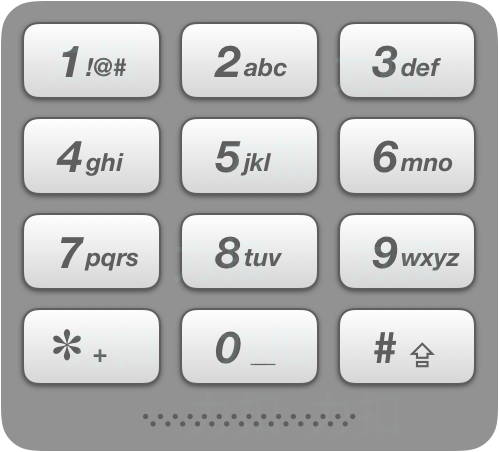
\includegraphics[width=50mm,height=50mm]{images/leetcode/17_telephone_keypad.png}

\textbf{示例}:

\begin{verbatim}
  输入:"23"
  输出:["ad", "ae", "af", "bd", "be", "bf", "cd", "ce", "cf"].
\end{verbatim}

\textbf{说明}: \\
尽管上面的答案是按字典序排列的,但是你可以任意选择答案输出的顺序。

\subsection{参考题解}

状态树如下,你只需要遍历整个树,把所有的叶子节点保存下来,
就是最终的结果。

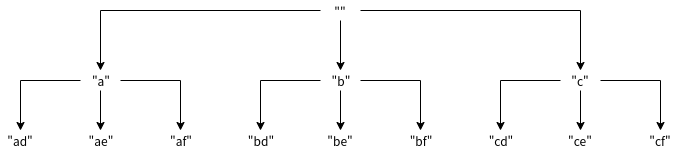
\includegraphics[width=150mm,height=40mm]{images/leetcode/leetcode_17.png}

\begin{verbatim}
/**
 * @param {string} digits
 * @return {string[]}
 */

const m = {
  '2': ['a', 'b', 'c'],
  '3': ['d', 'e', 'f'],
  '4': ['g', 'h', 'i'],
  '5': ['j', 'k', 'l'],
  '6': ['m', 'n', 'o'],
  '7': ['p', 'q', 'r', 's'],
  '8': ['t', 'u', 'v'],
  '9': ['w', 'x', 'y', 'z'],
};

var letterCombinations = function(digits) {
  if (digits.length === 0) { return []; }
  let result = [];
  dfs(result, "", digits);
  return result;
};

function dfs(result, node, digits) {
  if (digits.length === 0) {
    result.push(node);
    return;
  }
  let letters = m[digits[0]];
  for (let i = 0; i < letters.length; i += 1) {
    let letter = letters[i];
    dfs(result, node + letter, digits.substring(1));
  }
}
\end{verbatim}

\subsection{参考题解,分治回溯}

\begin{verbatim}
/**
 * @param {string} digits
 * @return {string[]}
 */
var letterCombinations = function(digits) {
  const m = {
    '2': ['a', 'b', 'c'],
    '3': ['d', 'e', 'f'],
    '4': ['g', 'h', 'i'],
    '5': ['j', 'k', 'l'],
    '6': ['m', 'n', 'o'],
    '7': ['p', 'q', 'r', 's'],
    '8': ['t', 'u', 'v'],
    '9': ['w', 'x', 'y', 'z'],
  };
  function recursion(digits) {
    if (digits.length === 0) {
      return [];
    }
    if (digits.length === 1) {
      return m[digits];
    }
    let result = [];
    let val = m[digits[0]];
    let sub = recursion(digits.substring(1));
    for (let i = 0; i < val.length; i += 1) {
      for (let j = 0; j < sub.length; j += 1) {
        result.push(val[i] + sub[j]);
      }
    }
    return result;
  }
  return recursion(digits);
};
\end{verbatim}

\newpage
\section{20. 有效的括号}
\label{leetcode:20}

\begin{verbatim}
/**
 * @param {string} s
 * @return {boolean}
 */
var isValid = function(s) {
  let stack = [];
  for (let c of s) {
    if (c === '(') {
      stack.push(')');
    } else if (c === '[') {
      stack.push(']');
    } else if (c === '{') {
      stack.push('}');
    } else if (c !== stack.pop()) {
      return false;
    }
  }
  return stack.length === 0;
};
\end{verbatim}

\newpage
\section{21. 合并两个有序链表}
\label{leetcode:21}

\begin{verbatim}
/**
 * Definition for singly-linked list.
 * function ListNode(val) {
 *     this.val = val;
 *     this.next = null;
 * }
 */
/**
 * @param {ListNode} l1
 * @param {ListNode} l2
 * @return {ListNode}
 */
var mergeTwoLists = function(l1, l2) {
  let dummy = new ListNode();
  let cur = dummy;
  let p1 = l1;
  let p2 = l2;
  while (p1 !== null && p2 !== null) {
    if (p1.val < p2.val) {
      cur.next = p1;
      p1 = p1.next;
    } else {
      cur.next = p2;
      p2 = p2.next;
    }
    cur = cur.next;
  }
  if (p1 !== null) { cur.next = p1; }
  if (p2 !== null) { cur.next = p2; }
  return dummy.next;
};
\end{verbatim}

\newpage
\section{22. 括号生成}
\label{leetcode:22}

\begin{verbatim}
/**
 * @param {number} n
 * @return {string[]}
 */
var generateParenthesis = function(n) {
  let result = [];
  recursion(result, 0, 0, n, "");
  return result;
};

function recursion(result, left, right, n, strs) {
  if (left === n && right === n) {
    result.push(strs);
    return;
  }
  if (left < n) {
    recursion(result, left + 1, right, n, strs + "(");
  }
  if (right < left) {
    recursion(result, left, right + 1, n, strs + ")");
  }
}
\end{verbatim}

\newpage
\section{24. 两两交换链表中的节点}
\label{leetcode:24}

\subsection{题目}

给定一个链表,两两交换其中相邻的节点,并返回交换后的链表。

\textbf{你不能只是单纯的改变节点内部的值},而是需要实际的进行节点交换。

\textbf{示例}:

\begin{verbatim}
  给定 1->2->3->4, 你应该返回 2->1->4->3.
\end{verbatim}

\subsection{参考题解}

链表题,画图即可理解。

\begin{verbatim}
/**
 * Definition for singly-linked list.
 * function ListNode(val) {
 *     this.val = val;
 *     this.next = null;
 * }
 */
/**
 * @param {ListNode} head
 * @return {ListNode}
 */
var swapPairs = function(head) {
  let dummy = new ListNode();
  dummy.next = head;
  let pre = dummy;
  let cur = head;
  while (cur !== null && cur.next !== null) {
    let post = cur.next;
    cur.next = post.next;
    post.next = cur;
    pre.next = post;
    pre = cur;
    cur = cur.next;
  }
  return dummy.next;
};
\end{verbatim}

\newpage
\section{25. K 个一组翻转链表}
\label{leetcode:25}

\subsection{题目}

给你一个链表,每 k 个节点一组进行翻转,请你返回翻转后的链表。

k 是一个正整数,它的值小于或等于链表的长度。

如果节点总数不是 k 的整数倍,那么请将最后剩余的节点保持原有顺序。

\textbf{示例}:

\begin{verbatim}
  给定这个链表:1->2->3->4->5
  当 k = 2 时,应当返回: 2->1->4->3->5
  当 k = 3 时,应当返回: 3->2->1->4->5
\end{verbatim}

\textbf{说明}:

\begin{itemize}
  \item 你的算法只能使用常数的额外空间。
  \item 你不能只是单纯的改变节点内部的值,而是需要实际的进行节点交换。
\end{itemize}

\subsection{参考题解}

\begin{verbatim}
/**
 * Definition for singly-linked list.
 * function ListNode(val) {
 *     this.val = val;
 *     this.next = null;
 * }
 */
/**
 * @param {ListNode} head
 * @param {number} k
 * @return {ListNode}
 */
var reverseKGroup = function(head, k) {
  const dummy = new ListNode();
  dummy.next = head;
  let pre = dummy;
  let end = dummy;
  while (end.next !== null) {
    for (let i = 0; i < k && end !== null; i += 1) {
      end = end.next;
    }
    if (end === null) {
      break;
    }

    let start = pre.next;
    let next = end.next;
    end.next = null;
    pre.next = reverseList(start);
    start.next = next;

    pre = start;
    end = pre;
  }
  return dummy.next;
};

var reverseList = function(head) {
  let [pre, cur] = [null, head];
  while (cur !== null) {
    let next = cur.next;
    cur.next = pre;
    pre = cur;
    cur = next;
  }
  return pre;
};
\end{verbatim}

\newpage
\section{26. 删除排序数组中的重复项}
\label{leetcode:26}

\subsection{题目}

给定一个排序数组,你需要在\textbf{原地}删除重复出现的元素,使得每个元素只出现一次,返回移除后数组的新长度。

不要使用额外的数组空间,你必须在\textbf{原地}修改输入数组并在使用 O(1) 额外空间的条件下完成。

\textbf{示例 1}:

\begin{verbatim}
  给定数组 nums = [1,1,2], 

  函数应该返回新的长度 2, 并且原数组 nums 的前两个元素被修改为 1, 2。 

  你不需要考虑数组中超出新长度后面的元素。
\end{verbatim}

\textbf{示例 2}:

\begin{verbatim}
  给定 nums = [0,0,1,1,1,2,2,3,3,4],

  函数应该返回新的长度 5, 并且原数组 nums 的前五个元素被修改为 0, 1, 2, 3, 4。

  你不需要考虑数组中超出新长度后面的元素。
\end{verbatim}

\subsection{参考题解}

\begin{verbatim}
/**
 * @param {number[]} nums
 * @return {number}
 */
var removeDuplicates = function(nums) {
  let lastUniqIndex = 0;
  for (let i = 1; i < nums.length; i += 1) {
    if (nums[i] === nums[lastUniqIndex]) {
      continue;
    }
    lastUniqIndex += 1;
    nums[lastUniqIndex] = nums[i];
  }
  return lastUniqIndex + 1;
};
\end{verbatim}

\newpage
\section{32. 最长有效括号}
\label{leetcode:32}

\newpage
\section{33. 搜索旋转排序数组}
\label{leetcode:33}

\subsection{题目}

假设按照升序排序的数组在预先未知的某个点上进行了旋转。

( 例如,数组 [0,1,2,4,5,6,7] 可能变为 [4,5,6,7,0,1,2] )。

搜索一个给定的目标值,如果数组中存在这个目标值,则返回它的索引,否则返回 -1 。

你可以假设数组中不存在重复的元素。

你的算法时间复杂度必须是 O(log n) 级别。

\textbf{示例 1}:

\begin{verbatim}
  输入: nums = [4,5,6,7,0,1,2], target = 0
  输出: 4
\end{verbatim}

\textbf{示例 2}:

\begin{verbatim}
  输入: nums = [4,5,6,7,0,1,2], target = 3
  输出: -1
\end{verbatim}

\subsection{参考题解,二分查找1}

nums = [7,8,9,1,2,3,4,5,6]

如果 target = 8,那我们把数组修改为:\\
\verb|[7,8,9,inf,inf,inf,inf,inf,inf]| \\
inf 表示无穷大,那这样我们就可以用二分查找了。

如果 target = 5,那我们把数组修改为:\\
\verb|[-inf,-inf,-inf,1,2,3,4,5,6]| \\
-inf 表示负无穷大,那这样我们就可以用二分查找了。

我们不需要真的去修改数组,只要每次计算 mid 中间那个数字的时候,
判断下 mid 和 target 是否在同一侧。如果在同一侧的话,就直接
判断即可,如果不在同一侧的话,把 mid 修改为 inf 或者 -inf 即可。

举例说明:

[7,8,9,1,2,3,4,5,6] \\
mid = 2, target = 6,在同一侧,所以 mid 不用修改。\\
mid = 2, target = 9,不在同一侧,把 mid 修改为 inf。

[4,5,6,7,8,9,1,2,3] \\
mid = 8,target = 9,在同一侧,所以 mid 不用修改。\\
mid = 8,target = 2,不在同一侧,把 mid 修改为 -inf。

那现在有两个问题。\\
1. 怎么判断是否在同一侧? \\
2. 怎么判断 mid 要修改为 inf 还是 -inf?

判断 mid 和 target 是否在同一侧,只需要和 nums[0] 对比即可。
如果 mid 和 target 都比 nums[0] 小,或者都比 nums[0] 大,
那他们就是在同一侧,否则就不在同一侧。

判断要修改为 inf 还是 -inf,就是把 target 和 nums[0] 对比即可。
如果 target < nums[0],说明 target 是在右侧,mid 则在左侧,
所以把 mid 修改为 -inf。那如果 target > nums[0],说明 target 在
左侧,mid 在右侧,所以把 mid 修改为 inf。

\subsubsection{Java}

\begin{verbatim}
class Solution {
  public int search(int[] nums, int target) {
    int left = 0;
    int right = nums.length - 1;
    while (left <= right) {
      int mid = left + (right - left) / 2;
      int num = (nums[mid] < nums[0]) == (target < nums[0])
        ? nums[mid]
        : target < nums[0] ? -Integer.MAX_VALUE : Integer.MAX_VALUE;
      if (num == target) {
        return mid;
      } else if (num > target) {
        right = mid - 1;
      } else {
        left = mid + 1;
      }
    }
    return -1;
  }
}
\end{verbatim}

\subsubsection{JavaScript}

\begin{verbatim}
/**
 * @param {number[]} nums
 * @param {number} target
 * @return {number}
 */
var search = function(nums, target) {
  let left = 0;
  let right = nums.length - 1;
  while (left <= right) {
    let mid = left + Math.floor((right - left) / 2);
    let num = (nums[mid] < nums[0]) === (target < nums[0])
      ? nums[mid]
      : target < nums[0] ? -Number.MAX_VALUE : Number.MAX_VALUE;
    if (num < target) {
      left = mid + 1;
    } else if (num > target) {
      right = mid - 1;
    } else {
      return mid;
    }
  }
  return -1;
};
\end{verbatim}

\subsection{参考题解,二分查找2}

先用二分查找找到最小的那个数字,也就是数组的转折的那个点。
然后再用一次二分查找来找到 target。

\begin{verbatim}
/**
 * @param {number[]} nums
 * @param {number} target
 * @return {number}
 */
var search = function(nums, target) {
  let rot = findSmallestIndex(nums);
  let left = 0;
  let right = nums.length - 1;
  while (left <= right) {
    let mid = left + Math.floor((right - left) / 2);
    let realMid = (mid + rot) % nums.length;
    if (nums[realMid] === target) {
      return realMid;
    } else if (nums[realMid] < target) {
      left = mid + 1;
    } else {
      right = mid - 1;
    }
  }
  return -1;
};

function findSmallestIndex(nums) {
  let [left, right] = [0, nums.length - 1];
  while (left < right) {
    let mid = left + Math.floor((right - left) / 2);
    if (nums[mid] > nums[right]) {
      left = mid + 1;
    } else {
      right = mid;
    }
  }
  return left;
}
\end{verbatim}

\newpage
\section{36. 有效的数独}
\label{leetcode:36}

\subsection{题目}

判断一个 9x9 的数独是否有效。只需要\textbf{根据以下规则},验证已经填入的数字是否有效即可。

\begin{enumerate}
  \item 数字 1-9 在每一行只能出现一次。
  \item 数字 1-9 在每一列只能出现一次。
  \item 数字 1-9 在每一个以粗实线分隔的 3x3 宫内只能出现一次。
\end{enumerate}

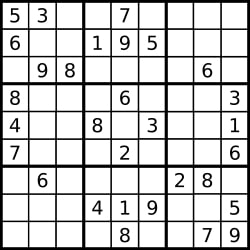
\includegraphics[width=60mm,height=60mm]{images/leetcode/36_sudo.jpg}

上图是一个部分填充的有效的数独。

数独部分空格内已填入了数字,空白格用 \verb|'.'| 表示。

\textbf{示例 1}:

\begin{verbatim}
输入:
[
  ["5","3",".",".","7",".",".",".","."],
  ["6",".",".","1","9","5",".",".","."],
  [".","9","8",".",".",".",".","6","."],
  ["8",".",".",".","6",".",".",".","3"],
  ["4",".",".","8",".","3",".",".","1"],
  ["7",".",".",".","2",".",".",".","6"],
  [".","6",".",".",".",".","2","8","."],
  [".",".",".","4","1","9",".",".","5"],
  [".",".",".",".","8",".",".","7","9"]
]
输出: true
\end{verbatim}

\textbf{示例 2}:

\begin{verbatim}
输入:
[
  ["8","3",".",".","7",".",".",".","."],
  ["6",".",".","1","9","5",".",".","."],
  [".","9","8",".",".",".",".","6","."],
  ["8",".",".",".","6",".",".",".","3"],
  ["4",".",".","8",".","3",".",".","1"],
  ["7",".",".",".","2",".",".",".","6"],
  [".","6",".",".",".",".","2","8","."],
  [".",".",".","4","1","9",".",".","5"],
  [".",".",".",".","8",".",".","7","9"]
]
输出: false
解释: 除了第一行的第一个数字从 5 改为 8 以外,空格内其他数字均与 示例1 相同。
     但由于位于左上角的 3x3 宫内有两个 8 存在, 因此这个数独是无效的。
\end{verbatim}

\textbf{说明}:

\begin{itemize}
  \item 一个有效的数独(部分已被填充)不一定是可解的。
  \item 只需要根据以上规则,验证已经填入的数字是否有效即可。
  \item 给定数独序列只包含数字 1-9 和字符 '.' 。
  \item 给定数独永远是 9x9 形式的。
\end{itemize}

\subsection{参考题解}

\subsubsection{Python}

\begin{verbatim}
class Solution:
  def isValidSudoku(self, board: List[List[str]]) -> bool:
    rows = len(board)
    cols = len(board[0])
    for row in range(rows):
      for col in range(cols):
        if board[row][col] == ".":
          continue
        c = board[row][col]
        board[row][col] = "."
        if not self.isValid(board, row, col, c):
          return False
        board[row][col] = c
    return True

  def isValid(self, board, row, col, c):
    for i in range(9):
      if board[i][col] == c:
        return False
      if board[row][i] == c:
        return False
      if board[row // 3 * 3 + i // 3][col // 3 * 3 + i % 3] == c:
        return False
    return True
\end{verbatim}

\newpage
\section{37. 解数独}
\label{leetcode:37}

\subsection{题目}

编写一个程序,通过已填充的空格来解决数独问题。

一个数独的解法需遵循如下规则:

\begin{enumerate}
  \item 数字 1-9 在每一行只能出现一次。
  \item 数字 1-9 在每一列只能出现一次。
  \item 数字 1-9 在每一个以粗实线分隔的 3x3 宫内只能出现一次。
\end{enumerate}

空白格用 \verb|'.'| 表示。

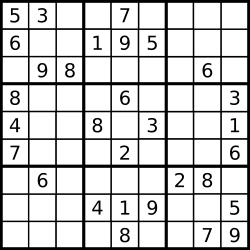
\includegraphics[width=60mm,height=60mm]{images/leetcode/37_sudo.png}

一个数独。

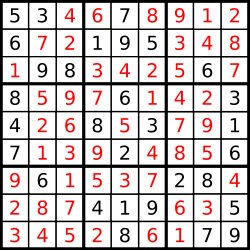
\includegraphics[width=60mm,height=60mm]{images/leetcode/37_sudo_solution.png}

答案被标成红色。

\textbf{Note}:

\begin{itemize}
  \item 给定的数独序列只包含数字 1-9 和字符 \verb|'.'| 。
  \item 你可以假设给定的数独只有唯一解。
  \item 给定数独永远是 9x9 形式的。
\end{itemize}

\subsection{参考题解}

\subsubsection{Python}

\begin{verbatim}
class Solution:
  def solveSudoku(self, board: List[List[str]]) -> None:
    """
    Do not return anything, modify board in-place instead.
    """
    self.board = board
    self.rows = len(board)
    self.cols = len(board[0])
    self.solve()

  def solve(self):
    for row in range(self.rows):
      for col in range(self.cols):
        if self.board[row][col] != ".":
          continue
        for num in ["1","2","3","4","5","6","7","8","9"]:
          if self.isValid(row, col, num):
            self.board[row][col] = num
            if self.solve():
              return True
            self.board[row][col] = "."
        return False
    return True

  def isValid(self, row, col, c):
    for i in range(9):
      if self.board[i][col] == c:
        return False
      if self.board[row][i] == c:
        return False
      if self.board[row // 3 * 3 + i // 3][col // 3 * 3 + i % 3] == c:
        return False
    return True
\end{verbatim}

\newpage
\section{42. 接雨水}
\label{leetcode:42}

\subsection{题目}

给定 n 个非负整数表示每个宽度为 1 的柱子的高度图,
计算按此排列的柱子,下雨之后能接多少雨水。

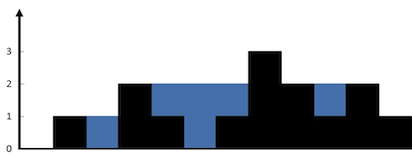
\includegraphics[width=100mm,height=50mm]{images/leetcode/rainwatertrap.png}

上面是由数组 [0,1,0,2,1,0,1,3,2,1,2,1] 表示的高度图,
在这种情况下,可以接 6 个单位的雨水(蓝色部分表示雨水)。\textbf{感谢 Marcos} 贡献此图。

\textbf{示例}:

\begin{verbatim}
  输入: [0,1,0,2,1,0,1,3,2,1,2,1]
  输出: 6
\end{verbatim}

\subsection{参考题解,栈}

用栈保存一个下降的序列。

\begin{verbatim}
/**
 * @param {number[]} height
 * @return {number}
 */
var trap = function(height) {
  var peek = function(stack) { return stack[stack.length - 1]; };
  let result = 0;
  let stack = [];
  for (let i = 0; i < height.length; i += 1) {
    while (stack.length > 0 && height[i] > height[peek(stack)]) {
      const top = stack.pop();
      if (stack.length === 0) {
        break;
      }
      let curWidth = i - peek(stack) - 1;
      let curHeight = Math.min(height[i], height[peek(stack)]) - height[top];
      let curArea = curWidth * curHeight;
      result += curArea;
    }
    stack.push(i);
  }
  return result;
};
\end{verbatim}

\newpage
\section{44. 通配符匹配}
\label{leetcode:44}

\subsection{题目}

\newpage
\section{45. 跳跃游戏 II}
\label{leetcode:45}

\subsection{题目}

给定一个非负整数数组,你最初位于数组的第一个位置。

数组中的每个元素代表你在该位置可以跳跃的最大长度。

你的目标是使用最少的跳跃次数到达数组的最后一个位置。

\textbf{示例}:

\begin{verbatim}
  输入: [2,3,1,1,4]
  输出: 2
  解释: 跳到最后一个位置的最小跳跃数是 2。
    从下标为 0 跳到下标为 1 的位置,跳 1 步,
  然后跳 3 步到达数组的最后一个位置。
\end{verbatim}

\textbf{说明}:

假设你总是可以到达数组的最后一个位置。

\subsection{参考题解,贪心法}

\newpage
\section{46. 全排列}
\label{leetcode:46}

\begin{verbatim}
/**
 * @param {number[]} nums
 * @return {number[][]}
 */
var permute = function(nums) {
  let result = [];
  recursion(nums, 0, result);
  return result;
};

function recursion(nums, first, result) {
  if (first === nums.length) {
    result.push(nums.slice());
  }

  for (let i = first; i < nums.length; i += 1) {
    [nums[first], nums[i]] = [nums[i], nums[first]];
    recursion(nums, first + 1, result);
    [nums[first], nums[i]] = [nums[i], nums[first]];
  }
}
\end{verbatim}
\newpage
\section{47. 全排列 II}
\label{leetcode:47}

\subsection{题目}

给定一个可包含重复数字的序列,返回所有不重复的全排列。

\textbf{示例}:

\begin{verbatim}
  输入: [1,1,2]
  输出:
  [
    [1,1,2],
    [1,2,1],
    [2,1,1]
  ]
\end{verbatim}

\subsection{参考题解}

\begin{verbatim}
/**
 * @param {number[]} nums
 * @return {number[][]}
 */
var permuteUnique = function(nums) {
  let result = [];
  let m = counter(nums);
  recursion(nums, m, [], result);
  return result;
};

function recursion(nums, m, cur, result) {
  if (cur.length === nums.length) {
    result.push(cur.map(e => +e));
    return;
  }

  for (let num in m) {
    if (m[num] > 0) {
      cur.push(num);
      m[num] -= 1;

      recursion(nums, m, cur, result);

      cur.pop();
      m[num] += 1;
    }
  }
}

function counter(nums) {
  const m = {};
  for (let i = 0; i < nums.length; i += 1) {
    const num = nums[i];
    if (num in m) {
      m[num] += 1;
    } else {
      m[num] = 1;
    }
  }
  return m;
}
\end{verbatim}
\newpage
\section{49. 字母异位词分组}
\label{leetcode:49}

\begin{verbatim}
/**
 * @param {string[]} strs
 * @return {string[][]}
 */
var groupAnagrams = function(strs) {
  const m = {};
  for (let i = 0; i < strs.length; i += 1) {
    const str = strs[i];
    const key = str.split("").sort().join("");
    if (key in m) {
      m[key].push(str);
    } else {
      m[key] = [str];
    }
  }

  const result = [];
  for (let key in m) {
    result.push(m[key]);
  }
  return result;
};
\end{verbatim}
\newpage
\section{50. Pow(x, n)}
\label{leetcode:50}

\newpage
\section{51. N皇后}
\label{leetcode:51}

\newpage
\section{52. N皇后 II}
\label{leetcode:52}

\subsection{题目}

n 皇后问题研究的是如何将 n 个皇后放置在 n×n 的棋盘上,并且使皇后彼此之间不能相互攻击。

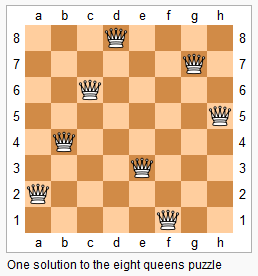
\includegraphics[width=50mm,height=50mm]{images/leetcode/8-queens.png}

上图为 8 皇后问题的一种解法。

给定一个整数 n,返回 n 皇后不同的解决方案的数量。

\textbf{示例}:

\begin{verbatim}
输入: 4
输出: 2
解释: 4 皇后问题存在如下两个不同的解法。
[
 [".Q..",  // 解法 1
  "...Q",
  "Q...",
  "..Q."],

 ["..Q.",  // 解法 2
  "Q...",
  "...Q",
  ".Q.."]
]
\end{verbatim}

\subsection{参考题解}

\begin{verbatim}
class Solution:
  def totalNQueens(self, n: int) -> int:
    self.count = 0
    def dfs(cols, pie, na, row):
      if row >= n:
        self.count += 1
        return
      for col in range(n):
        if (col not in cols) and (row + col not in pie) and (row - col not in na):
          dfs(cols|{col}, pie|{row+col}, na|{row-col}, row+1)
    dfs(set(), set(), set(), 0)
    return self.count
\end{verbatim}

\subsection{参考题解,位运算}

列,撇,捺 这 3 个 set 可以用位运算来优化,只需要用一个整数即可。

\begin{verbatim}
class Solution:
  def totalNQueens(self, n: int) -> int:
    self.count = 0
    def dfs(cols, pie, na, row):
      if row >= n:
        self.count += 1
        return
      bits = (~(cols|pie|na)) & ((1<<n) - 1) # 得到当前所有的空位
      while bits:
        p = bits & -bits # 取到最低位的1
        bits = bits & (bits - 1) # 表示在p位置上放入皇后
        dfs(cols|p, (pie|p)<<1, (na|p)>>1, row+1)
    dfs(0, 0, 0, 0)
    return self.count
\end{verbatim}

\newpage
\section{53. 最大子序和}
\label{leetcode:53}

\newpage
\section{55. 跳跃游戏}
\label{leetcode:55}

\subsection{题目}

给定一个非负整数数组,你最初位于数组的第一个位置。

数组中的每个元素代表你在该位置可以跳跃的最大长度。

判断你是否能够到达最后一个位置。

\textbf{示例 1}:

\begin{verbatim}
  输入: [2,3,1,1,4]
  输出: true
  解释: 我们可以先跳 1 步,从位置 0 到达 位置 1, 
  然后再从位置 1 跳 3 步到达最后一个位置。
\end{verbatim}

\textbf{示例 2}:

\begin{verbatim}
  输入: [3,2,1,0,4]
  输出: false
  解释: 无论怎样,你总会到达索引为 3 的位置。
  但该位置的最大跳跃长度是 0 , 所以你永远不可能到达最后一个位置。
\end{verbatim}

\subsection{参考题解,贪心法}

\begin{verbatim}
/**
 * @param {number[]} nums
 * @return {boolean}
 */
var canJump = function(nums) {
  let lastPos = nums.length - 1;
  for (let i = nums.length - 1; i >= 0; i -= 1) {
    if (i + nums[i] >= lastPos) {
      lastPos = i;
    }
  }
  return lastPos === 0;
};
\end{verbatim}

\newpage
\section{56. 合并区间}
\label{leetcode:56}

\subsection{题目}

给出一个区间的集合,请合并所有重叠的区间。

\textbf{示例 1}:

\begin{verbatim}
  输入: [[1,3],[2,6],[8,10],[15,18]]
  输出: [[1,6],[8,10],[15,18]]
  解释: 区间 [1,3] 和 [2,6] 重叠, 将它们合并为 [1,6].
\end{verbatim}

\textbf{示例 2}:

\begin{verbatim}
  输入: [[1,4],[4,5]]
  输出: [[1,5]]
  解释: 区间 [1,4] 和 [4,5] 可被视为重叠区间。
\end{verbatim}

\subsection{参考题解,Python}

\begin{verbatim}
class Solution:
  def merge(self, intervals: List[List[int]]) -> List[List[int]]:
    intervals.sort(key=lambda x: x[0])
    result = []
    for interval in intervals:
      if not result:
        result.append(interval)
      elif result[-1][1] < interval[0]:
        result.append(interval)
      else:
        result[-1][1] = max(result[-1][1], interval[1])
    return result
\end{verbatim}

\newpage
\section{58. 最后一个单词的长度}
\label{leetcode:58}

\subsection{题目}

给定一个仅包含大小写字母和空格 \verb|' '| 的字符串 s,返回其最后一个单词的长度。

如果字符串从左向右滚动显示,那么最后一个单词就是最后出现的单词。

如果不存在最后一个单词,请返回 0 。

说明:一个单词是指仅由字母组成、不包含任何空格的 最大子字符串。

\textbf{示例}:

\begin{verbatim}
  输入: "Hello World"
  输出: 5
\end{verbatim}

\subsection{参考题解}

\subsubsection{Python}

\begin{verbatim}
class Solution:
  def lengthOfLastWord(self, s: str) -> int:
    strs = s.split()
    return len(strs[-1]) if strs else 0
\end{verbatim}

\newpage
\section{62. 不同路径}
\label{leetcode:62}

\newpage
\section{63. 不同路径 II}
\label{leetcode:63}

\newpage
\section{64. 最小路径和}
\label{leetcode:64}

\newpage
\section{66. 加一}
\label{leetcode:66}

\subsection{题目}

给定一个由\textbf{整数}组成的\textbf{非空}数组所表示的非负整数,在该数的基础上加一。

最高位数字存放在数组的首位, 数组中每个元素只存储\textbf{单个}数字。

你可以假设除了整数 0 之外,这个整数不会以零开头。

\textbf{示例 1}:

\begin{verbatim}
  输入: [1,2,3]
  输出: [1,2,4]
  解释: 输入数组表示数字 123。
\end{verbatim}

\textbf{示例 2}:

\begin{verbatim}
  输入: [4,3,2,1]
  输出: [4,3,2,2]
  解释: 输入数组表示数字 4321。
\end{verbatim}

\subsection{参考题解}

\begin{verbatim}
/**
 * @param {number[]} digits
 * @return {number[]}
 */
var plusOne = function(digits) {
  let carry = 1;
  for (let i = digits.length - 1; i >= 0; i -= 1) {
    digits[i] += carry;
    carry = Math.floor(digits[i] / 10);
    digits[i] = digits[i] % 10;
  }
  if (carry > 0) { digits.unshift(carry); }
  return digits;
};
\end{verbatim}

\newpage
\section{69. x 的平方根}
\label{leetcode:69}

\subsection{题目}

实现 int sqrt(int x) 函数。

计算并返回 x 的平方根,其中 x 是非负整数。

由于返回类型是整数,结果只保留整数的部分,小数部分将被舍去。

\textbf{示例 1}:

\begin{verbatim}
  输入: 4
  输出: 2
\end{verbatim}

\textbf{示例 2}:

\begin{verbatim}
  输入: 8
  输出: 2
  说明: 8 的平方根是 2.82842..., 
       由于返回类型是整数,小数部分将被舍去。
\end{verbatim}

\subsection{参考题解,二分法}

\begin{verbatim}
/**
 * @param {number} x
 * @return {number}
 */
var mySqrt = function(x) {
  return Math.floor(MySqrt(x, 0.01));
};

function MySqrt(x, precision) {
  if (x === 0 || x === 1) {
    return x;
  }

  let left = 0;
  let right = x;
  while (left <= right) {
    let mid = (left + right) / 2;
    let cur = mid * mid;
    if (cur - x >= -precision && cur - x <= precision) {
      return mid;
    } else if (cur > x) {
      right = mid;
    } else {
      left = mid;
    }
  }
  return null;
}
\end{verbatim}

\subsection{参考题解,牛顿迭代法}

\begin{verbatim}
/**
* @param {number} x
* @return {number}
*/
var mySqrt = function(x) {
  let r = x;
  while (r * r > x) {
    r = Math.floor((r + Math.floor(x / r)) / 2);
  }
  return r;
};
\end{verbatim}

\subsection{扩展,雷神之锤}

\begin{verbatim}
float InvSqrt (float x){
  float xhalf = 0.5f*x;
  int i = *(int*)&x;
  i = 0x5f3759df - (i>>1);
  x = *(float*)&i;
  x = x*(1.5f - xhalf*x*x);
  return x;
}
\end{verbatim}

\newpage
\section{70. 爬楼梯}
\label{leetcode:70}

\subsection{题目}

假设你正在爬楼梯。需要 n 阶你才能到达楼顶。

每次你可以爬 1 或 2 个台阶。你有多少种不同的方法可以爬到楼顶呢?

\textbf{注意}:给定 n 是一个正整数。

\textbf{示例 1}:

\begin{verbatim}
  输入: 2
  输出: 2
  解释: 有两种方法可以爬到楼顶。
  1.  1 阶 + 1 阶
  2.  2 阶
\end{verbatim}

\textbf{示例 2}:

\begin{verbatim}
  输入: 3
  输出: 3
  解释: 有三种方法可以爬到楼顶。
  1.  1 阶 + 1 阶 + 1 阶
  2.  1 阶 + 2 阶
  3.  2 阶 + 1 阶
\end{verbatim}

\subsection{参考题解}

\begin{verbatim}
/**
 * @param {number} n
 * @return {number}
 */
var climbStairs = function(n) {
  if (n < 3) {
    return n;
  }
  let [f1, f2] = [1, 2];
  for (let i = 3; i <= n; i += 1) {
    [f1, f2] = [f2, f1 + f2];
  }
  return f2;
};
\end{verbatim}

\newpage
\section{72. 编辑距离}
\label{leetcode:72}

\subsection{题目}

给定两个单词 word1 和 word2,计算出将 word1 转换成 word2 所使用的最少操作数。

你可以对一个单词进行如下三种操作:

\begin{itemize}
  \item 插入一个字符
  \item 删除一个字符
  \item 替换一个字符
\end{itemize}

\textbf{示例 1}:

\begin{verbatim}
  输入: word1 = "horse", word2 = "ros"
  输出: 3
  解释:
  horse -> rorse (将 'h' 替换为 'r')
  rorse -> rose (删除 'r')
  rose -> ros (删除 'e')
\end{verbatim}

\textbf{示例 2}:

\begin{verbatim}
  输入: word1 = "intention", word2 = "execution"
  输出: 5
  解释:
  intention -> inention (删除 't')
  inention -> enention (将 'i' 替换为 'e')
  enention -> exention (将 'n' 替换为 'x')
  exention -> exection (将 'n' 替换为 'c')
  exection -> execution (插入 'u')
\end{verbatim}

\subsection{参考题解,JavaScript 代码}

这个题目要照着代码把 dp 的二维数组自己画下,就知道怎么回事了。

\begin{verbatim}
/**
* @param {string} word1
* @param {string} word2
* @return {number}
*/
var minDistance = function(word1, word2) {
  let rows = word1.length+1;
  let cols = word2.length+1;
  let dp = new Array(rows).fill(null).map(() => {
    return new Array(cols).fill(0);
  });
  for (let row = 1; row < rows; row += 1) {
    dp[row][0] = row;
  }
  for (let col = 1; col < cols; col += 1) {
    dp[0][col] = col;
  }
  for (let row = 1; row < rows; row += 1) {
    for (let col = 1; col < cols; col += 1) {
      if (word1[row-1] == word2[col-1]) {
        dp[row][col] = 1 + Math.min(dp[row-1][col],
          dp[row][col-1], dp[row-1][col-1]-1);
      } else {
        dp[row][col] = 1 + Math.min(dp[row-1][col],
          dp[row][col-1], dp[row-1][col-1]);
      }
    }
  }
  return dp[word1.length][word2.length];
};
\end{verbatim}

\subsection{参考题解,Python 代码}

\begin{verbatim}
class Solution:
  def minDistance(self, word1: str, word2: str) -> int:
    rows = len(word1) + 1
    cols = len(word2) + 1
    dp = [[0 for _ in range(cols)] for _ in range(rows)]
    for row in range(1, rows):
      dp[row][0] = dp[row-1][0] + 1
    for col in range(1, cols):
      dp[0][col] = col
    for row in range(1, rows):
      for col in range(1, cols):
        if word1[row-1] == word2[col-1]:
          dp[row][col] = 1 + min(dp[row-1][col], dp[row][col-1],
              dp[row-1][col-1] - 1)
        else:
          dp[row][col] = 1 + min(dp[row-1][col], dp[row][col-1],
              dp[row-1][col-1])
    return dp[-1][-1]
\end{verbatim}

\newpage
\section{74. 搜索二维矩阵}
\label{leetcode:74}

\subsection{题目}

编写一个高效的算法来判断 m x n 矩阵中,是否存在一个目标值。该矩阵具有如下特性:

每行中的整数从左到右按升序排列。
每行的第一个整数大于前一行的最后一个整数。

\textbf{示例 1}:

\begin{verbatim}
  输入:
  matrix = [
    [1,   3,  5,  7],
    [10, 11, 16, 20],
    [23, 30, 34, 50]
  ]
  target = 3
  输出: true
\end{verbatim}

\textbf{示例 2}:

\begin{verbatim}
  输入:
  matrix = [
    [1,   3,  5,  7],
    [10, 11, 16, 20],
    [23, 30, 34, 50]
  ]
  target = 13
  输出: false
\end{verbatim}

\subsection{参考题解,二分查找}

\begin{verbatim}
/**
* @param {number[][]} matrix
* @param {number} target
* @return {boolean}
*/
var searchMatrix = function(matrix, target) {
  let rows = matrix.length;
  if (rows === 0) { return false; }
  let cols = matrix[0].length;
  let left = 0;
  let right = rows * cols - 1;
  while (left <= right) {
    let mid = left + Math.floor((right - left) / 2);
    let midRow = Math.floor(mid / cols);
    let midCol = mid % cols;
    if (matrix[midRow][midCol] === target) {
      return true;
    } else if (matrix[midRow][midCol] < target) {
      left = mid + 1;
    } else {
      right = mid - 1;
    }
  }
  return false;
};
\end{verbatim}

\newpage
\section{76. 最小覆盖子串}
\label{leetcode:76}

\subsection{题目}

给你一个字符串 S、一个字符串 T,请在字符串 S 里面找出:包含 T 所有字母的最小子串。

\textbf{示例}:

\begin{verbatim}
  输入: S = "ADOBECODEBANC", T = "ABC"
  输出: "BANC"
\end{verbatim}

\textbf{说明}:

\begin{itemize}
  \item 如果 S 中不存这样的子串,则返回空字符串 ``''。
  \item 如果 S 中存在这样的子串,我们保证它是唯一的答案。
\end{itemize}

\subsection{参考题解}

\subsubsection{JavaScript}

\begin{verbatim}
/**
* @param {string} s
* @param {string} t
* @return {string}
*/
var minWindow = function(s, t) {
  const m = {};
  let left = 0;
  let right = -1;
  let minStr = '';

  t.split('').forEach(element => {
    if (element in m) {
      m[element] += 1;
    } else {
      m[element] = 1;
    }
  })

  let count = Object.keys(m).length;

  while (right <= s.length) {
    if (count === 0) {
      let temp = s.substring(left, right + 1);
      if (minStr === '') {
        minStr = temp;
      } else {
        minStr = minStr.length < temp.length ? minStr : temp;
      }

      let current = s[left];
      if (current in m) {
        m[current] += 1;
      }
      if (m[current] > 0) {
        count += 1;
      }
      left += 1;

    } else {
      right += 1;
      let current = s[right];
      if (current in m) {
        m[current] -= 1;
      }
      if (m[current] === 0) {
        count -= 1;
      }
    }
  }

  return minStr;
};
\end{verbatim}

\subsection{参考题解}

\subsubsection{Python}

\begin{verbatim}
class Solution:
  def minWindow(self, s: str, t: str) -> str:
    m, cur = collections.Counter(t), {}
    count, left, right, minstr = len(m.keys()), 0, 0, ''
    while right < len(s) or left < len(s):
      if count == 0:
        curstr = s[left:right]
        if minstr == '' or len(curstr) < len(minstr):
          minstr = curstr
        c = s[left]
        if c in m:
          if cur[c] == m[c]:
            count += 1
          cur[c] -= 1
        left += 1
      else:
        if right >= len(s):
          break
        c = s[right]
        if c in m:
          if c in cur:
            cur[c] += 1
          else:
            cur[c] = 1
          if cur[c] == m[c]:
            count -=1
        right += 1
    return minstr
\end{verbatim}


\newpage
\section{77. 组合}
\label{leetcode:77}

\subsection{题目}

给定两个整数 n 和 k,返回 \verb|1 ... n| 中所有可能的 k 个数的组合。

\textbf{示例}:

\begin{verbatim}
  输入: n = 4, k = 2
  输出:
  [
    [2,4],
    [3,4],
    [2,3],
    [1,2],
    [1,3],
    [1,4],
  ]
\end{verbatim}

\subsection{参考题解}

n = 4, k = 2 时状态树如下:

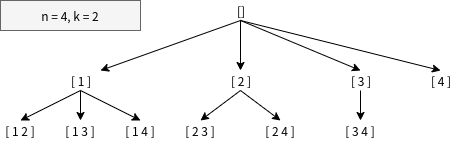
\includegraphics[width=100mm,height=50mm]{images/leetcode/leetcode_77.png}

n = 4, k = 3 时状态树如下:

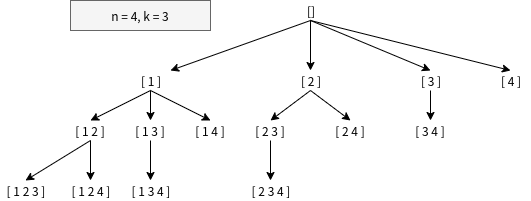
\includegraphics[width=100mm,height=50mm]{images/leetcode/leetcode_77_4_3.png}

遍历整个状态树,找到叶子节点中,数组长度等于 k 的节点,就是我们要的结果。

可以这么理解整个遍历的过程:

\begin{displaymath}
  \mathrm{C}_n^k = \mathrm{C}_{n-1}^{k-1} + \mathrm{C}_{n-1}^k
\end{displaymath}

$\mathrm{C}_n^k$ 表示在 n 个中取 k 个。
可以分为两种情况:

\begin{itemize}
  \item $\mathrm{C}_{n-1}^{k-1}$ 选择了第 n 个,然后我们只要在
    剩下的 n-1 个中选择 k-1 个。
  \item $\mathrm{C}_{n-1}^k$ 不选择第 n 个,那么我们需要在
    剩下的 n-1 个中选择 k 个。
\end{itemize}

\begin{verbatim}
/**
 * @param {number} n
 * @param {number} k
 * @return {number[][]}
 */
var combine = function(n, k) {
  let result = [];
  recursion(n, k, 1, [], result);
  return result;
};

function recursion(n, k, first, cur, result) {
  if (cur.length === k) {
    result.push(cur.slice())
    return;
  }

  for (let i = first; i <= n; i += 1) {
    cur.push(i);
    recursion(n, k, i + 1, cur, result);
    cur.pop();
  }
}
\end{verbatim}

\newpage
\section{78. 子集}
\label{leetcode:78}

\newpage
\section{84. 柱状图中最大的矩形}
\label{leetcode:84}

\subsection{题目}

给定 n 个非负整数,用来表示柱状图中各个柱子的高度。每个柱子彼此相邻,且宽度为 1 。

求在该柱状图中,能够勾勒出来的矩形的最大面积。

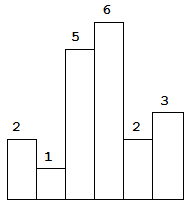
\includegraphics[width=50mm,height=50mm]{images/leetcode/histogram.png}

以上是柱状图的示例,其中每个柱子的宽度为 1,给定的高度为 [2,1,5,6,2,3]。

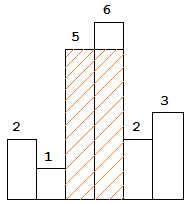
\includegraphics[width=50mm,height=50mm]{images/leetcode/histogram_area.png}

图中阴影部分为所能勾勒出的最大矩形面积,其面积为 10 个单位。

\textbf{示例}:

\begin{verbatim}
  输入: [2,1,5,6,2,3]
  输出: 10
\end{verbatim}

\subsection{参考题解,暴力法}

先用两重循环遍历出所有可能的左右边界组合。
比如我把左边界叫做 left,右边界叫做 right,
然后我们在 left 和 right 之间去找最矮的那根柱子,
那么面积就是 (right - left) * 最矮柱子的高度。

\begin{verbatim}
/**
 * @param {number[]} heights
 * @return {number}
 */
var largestRectangleArea = function(heights) {
  // 暴力解法,会超出时间限制。
  let maxarea = 0;
  const n = heights.length;
  for (let i = 0; i < n; i += 1) {
    for (let j = i; j < n; j += 1) {
      let minHeight = heights[i];
      for (let k = i; k <= j; k += 1) {
        if (heights[k] < minHeight) {
          minHeight = heights[k];
        }
      }
      const curarea = minHeight * (j - i + 1);
      if (curarea > maxarea) {
        maxarea = curarea;
      }
    }
  }
  return maxarea;
};
\end{verbatim}

\subsection{参考题解,栈}

用栈来保存一个上升的序列。

\begin{verbatim}
/**
 * @param {number[]} heights
 * @return {number}
 */
var largestRectangleArea = function(heights) {
  var peek = function(stack) { return stack[stack.length - 1]; };
  let stack = [-1];
  let maxarea = 0;
  for (let i = 0; i < heights.length; i += 1) {
    while (peek(stack) !== -1 && heights[i] <= heights[peek(stack)]) {
      const top = stack.pop();
      const curarea = heights[top] * (i - peek(stack) - 1);
      maxarea = Math.max(maxarea, curarea)
    }
    stack.push(i);
  }
  while (peek(stack) !== -1) {
    const top = stack.pop();
    const curarea = heights[top] * (heights.length - peek(stack) - 1);
    maxarea = Math.max(maxarea, curarea)
  }
  return maxarea;
};
\end{verbatim}

\newpage
\section{85. 最大矩形}
\label{leetcode:85}

\subsection{题目}

\newpage
\section{88. 合并两个有序数组}
\label{leetcode:88}

\subsection{题目}

给定两个有序整数数组 nums1 和 nums2,将 nums2 合并到 nums1 中,使得 num1 成为一个有序数组。

\textbf{说明}:

\begin{itemize}
  \item 初始化 nums1 和 nums2 的元素数量分别为 m 和 n。
  \item 你可以假设 nums1 有足够的空间(空间大小大于或等于 m + n)
    来保存 nums2 中的元素。
\end{itemize}

\textbf{示例}:

\begin{verbatim}
  输入:
  nums1 = [1,2,3,0,0,0], m = 3
  nums2 = [2,5,6],       n = 3

  输出: [1,2,2,3,5,6]
\end{verbatim}

\subsection{参考题解}

其实就是保存 3 个 index 下标,这 3 个 index 下标都是
从后往前遍历。

\begin{verbatim}
/**
 * @param {number[]} nums1
 * @param {number} m
 * @param {number[]} nums2
 * @param {number} n
 * @return {void} Do not return anything, 
 *   modify nums1 in-place instead.
 */
var merge = function(nums1, m, nums2, n) {
  let curIndex = m + n - 1;
  let idx1 = m - 1;
  let idx2 = n - 1;
  while (idx1 >= 0 && idx2 >= 0) {
    if (nums1[idx1] > nums2[idx2]) {
      nums1[curIndex--] = nums1[idx1--];
    } else {
      nums1[curIndex--] = nums2[idx2--];
    }
  }
  while (idx1 >= 0) { nums1[curIndex--] = nums1[idx1--]; }
  while (idx2 >= 0) { nums1[curIndex--] = nums2[idx2--]; }
};
\end{verbatim}

\newpage
\section{91. 解码方法}
\label{leetcode:91}

\newpage
\section{94. 二叉树的中序遍历}
\label{leetcode:94}

\subsection{题目}

给定一个二叉树,返回它的中序 遍历。

\textbf{示例}:

\begin{verbatim}
  输入: [1,null,2,3]
    1
      \
      2
      /
    3

  输出: [1,3,2]
\end{verbatim}

\textbf{进阶}: 递归算法很简单,你可以通过迭代算法完成吗?

\subsection{参考题解}

\begin{verbatim}
/**
 * Definition for a binary tree node.
 * function TreeNode(val) {
 *     this.val = val;
 *     this.left = this.right = null;
 * }
 */
/**
 * @param {TreeNode} root
 * @return {number[]}
 */
var inorderTraversal = function(root) {
  let result = [];
  recursion(root, result);
  return result;
};

function recursion(root, result) {
  if (root === null) { return; }
  recursion(root.left, result);
  result.push(root.val);
  recursion(root.right, result);
}
\end{verbatim}
\newpage
\section{98. 验证二叉搜索树}
\label{leetcode:98}

\subsection{题目}

给定一个二叉树,判断其是否是一个有效的二叉搜索树。

假设一个二叉搜索树具有如下特征:

\begin{enumerate}
  \item 节点的左子树只包含小于当前节点的数。
  \item 节点的右子树只包含大于当前节点的数。
  \item 所有左子树和右子树自身必须也是二叉搜索树。
\end{enumerate}

\textbf{示例 1}:

\begin{verbatim}
  输入:
     2
    / \
   1   3
  输出: true
\end{verbatim}

\textbf{示例 2}:

\begin{verbatim}
  输入:
     5
    / \
   1   4
      / \
     3   6
  输出: false
  解释: 输入为: [5,1,4,null,null,3,6]。
       根节点的值为 5 ,但是其右子节点值为 4 。
\end{verbatim}

\subsection{参考题解}

\subsubsection{JavaScript}

\begin{verbatim}
/**
 * Definition for a binary tree node.
 * function TreeNode(val) {
 *     this.val = val;
 *     this.left = this.right = null;
 * }
 */
/**
 * @param {TreeNode} root
 * @return {boolean}
 */
var isValidBST = function(root) {
  return isValid(root, null, null);
};

function isValid(root, min, max) {
  if (root === null) { return true; }
  if (min !== null && root.val <= min) { return false; }
  if (max !== null && root.val >= max) { return false; }
  return isValid(root.left, min, root.val) &&
    isValid(root.right, root.val, max);
}
\end{verbatim}

\subsubsection{Golang}

\begin{verbatim}
/**
* Definition for a binary tree node.
* type TreeNode struct {
*     Val int
*     Left *TreeNode
*     Right *TreeNode
* }
*/
func isValidBST(root *TreeNode) bool {
  return isValid(root, nil, nil)
}

func isValid(root, min, max *TreeNode) bool {
  if root == nil {
    return true
  }
  if min != nil && root.Val <= min.Val {
    return false
  }
  if max != nil && root.Val >= max.Val {
    return false
  }
  return isValid(root.Left, min, root) &&
    isValid(root.Right, root, max)
}
\end{verbatim}


\newpage
\section{102. 二叉树的层次遍历}
\label{leetcode:102}

\subsection{题目}

给定一个二叉树,返回其按层次遍历的节点值。 (即逐层地,从左到右访问所有节点)。

例如:
给定二叉树: [3,9,20,null,null,15,7],

\begin{verbatim}
   3
  / \
 9  20
   /  \
  15   7
\end{verbatim}

返回其层次遍历结果:

\begin{verbatim}
[
  [3],
  [9,20],
  [15,7]
]
\end{verbatim}

\subsection{参考题解,BFS}

\begin{verbatim}
/**
 * Definition for a binary tree node.
 * function TreeNode(val) {
 *     this.val = val;
 *     this.left = this.right = null;
 * }
 */
/**
 * @param {TreeNode} root
 * @return {number[][]}
 */
var levelOrder = function(root) {
  if (root === null) { return []; }
  let result = [];
  let queue = [];
  queue.push(root);
  while (queue.length > 0) {
    const levelSize = queue.length;
    const currentLevel = [];
    for (let i = 0; i < levelSize; i += 1) {
      let node = queue.shift();
      currentLevel.push(node.val);
      if (node.left) { queue.push(node.left); }
      if (node.right) { queue.push(node.right); }
    }
    result.push(currentLevel);
  }
  return result;
};
\end{verbatim}

\subsection{参考题解,DFS}

\begin{verbatim}
/**
 * Definition for a binary tree node.
 * function TreeNode(val) {
 *     this.val = val;
 *     this.left = this.right = null;
 * }
 */
/**
 * @param {TreeNode} root
 * @return {number[][]}
 */
var levelOrder = function(root) {
  if (root === null) { return []; }
  let result = [];
  dfs(result, root, 0);
  return result;
};

function dfs(result, node, level) {
  if (node === null) { return; }
  if (result.length < level + 1) { result.push([]); }
  result[level].push(node.val);
  dfs(result, node.left, level + 1);
  dfs(result, node.right, level + 1);
}
\end{verbatim}

\newpage
\section{104. 二叉树的最大深度}
\label{leetcode:104}

\begin{verbatim}
/**
 * Definition for a binary tree node.
 * function TreeNode(val) {
 *     this.val = val;
 *     this.left = this.right = null;
 * }
 */
/**
 * @param {TreeNode} root
 * @return {number}
 */
var maxDepth = function(root) {
  return root === null
    ? 0
    : 1 + Math.max(maxDepth(root.left), maxDepth(root.right));
};
\end{verbatim}
\newpage
\section{105. 从前序与中序遍历序列构造二叉树}
\label{leetcode:105}

\begin{verbatim}
/**
 * Definition for a binary tree node.
 * function TreeNode(val) {
 *     this.val = val;
 *     this.left = this.right = null;
 * }
 */
/**
 * @param {number[]} preorder
 * @param {number[]} inorder
 * @return {TreeNode}
 */
var buildTree = function(preorder, inorder) {
  if (preorder.length === 0 || inorder.length === 0) {
    return null;
  }
  let val = preorder[0];
  let idx = inorder.indexOf(val);
  let node = new TreeNode(val);
  node.left = buildTree(preorder.slice(1, 1+idx), inorder.slice(0, idx));
  node.right = buildTree(preorder.slice(1+idx), inorder.slice(idx+1));
  return node;
};
\end{verbatim}

\begin{verbatim}
/**
 * Definition for a binary tree node.
 * type TreeNode struct {
 *     Val int
 *     Left *TreeNode
 *     Right *TreeNode
 * }
 */
func buildTree(preorder []int, inorder []int) *TreeNode {
	if len(preorder) == 0 || len(inorder) == 0 {
		return nil
	}
	val := preorder[0]
	idx := index(inorder, val)
	node := &TreeNode{Val: val}
	node.Left = buildTree(preorder[1:idx+1], inorder[:idx])
	node.Right = buildTree(preorder[idx+1:], inorder[idx+1:])
	return node
}

func index(array []int, val int) int {
	for i := 0; i < len(array); i++ {
		if array[i] == val {
			return i
		}
	}
	return -1
}
\end{verbatim}
\newpage
\section{111. 二叉树的最小深度}
\label{leetcode:111}

\subsection{题目}

给定一个二叉树,找出其最小深度。

最小深度是从根节点到最近叶子节点的最短路径上的节点数量。

\textbf{说明}: 叶子节点是指没有子节点的节点。

\textbf{示例}:

给定二叉树 [3,9,20,null,null,15,7],

\begin{verbatim}
     3
    / \
   9  20
    /  \
   15   7
  返回它的最小深度 2.
\end{verbatim}

\subsection{参考题解}

\subsubsection{JavaScript}

\begin{verbatim}
/**
 * Definition for a binary tree node.
 * function TreeNode(val) {
 *     this.val = val;
 *     this.left = this.right = null;
 * }
 */
/**
 * @param {TreeNode} root
 * @return {number}
 */
var minDepth = function(root) {
  if (root === null) { return 0; }
  const left = minDepth(root.left);
  const right = minDepth(root.right);
  return left === 0 || right === 0
    ? left + right + 1
    : Math.min(left, right) + 1;
};
\end{verbatim}

\subsubsection{Golang}

\begin{verbatim}
/**
* Definition for a binary tree node.
* type TreeNode struct {
*     Val int
*     Left *TreeNode
*     Right *TreeNode
* }
*/
func minDepth(root *TreeNode) int {
  if root == nil {
    return 0
  }
  left := minDepth(root.Left)
  right := minDepth(root.Right)
  if left == 0 || right == 0 {
    return left + right + 1
  }
  if left < right {
    return left + 1
  }
  return right + 1
}
\end{verbatim}

\newpage
\section{120. 三角形最小路径和}
\label{leetcode:120}

\subsection{题目}

给定一个整数数组 nums ,找出一个序列中乘积最大的连续子序列(该序列至少包含一个数)。

\textbf{示例 1}:

\begin{verbatim}
  输入: [2,3,-2,4]
  输出: 6
  解释: 子数组 [2,3] 有最大乘积 6。
\end{verbatim}

\textbf{示例 2}:

\begin{verbatim}
  输入: [-2,0,-1]
  输出: 0
  解释: 结果不能为 2, 因为 [-2,-1] 不是子数组。
\end{verbatim}

\subsection{参考题解}

\begin{verbatim}
/**
* @param {number[][]} triangle
* @return {number}
*/
var minimumTotal = function(triangle) {
  // dp[row][col] = min(dp[row+1][col], dp[row+1][col+1]) + triangle[row][col]
  for (let row = triangle.length - 2; row >= 0; row -= 1) {
    for (let col = 0; col < triangle[row].length; col += 1) {
      triangle[row][col] = Math.min(triangle[row+1][col],
        triangle[row+1][col+1]) + triangle[row][col];
    }
  }
  return triangle[0][0];
};
\end{verbatim}

\newpage
\section{121. 买卖股票的最佳时机}
\label{leetcode:121}

\newpage
\section{122. 买卖股票的最佳时机 II}
\label{leetcode:122}

\newpage
\section{123. 买卖股票的最佳时机 III}
\label{leetcode:123}

\newpage
\section{126. 单词接龙 II}
\label{leetcode:126}

\subsection{题目}

给定两个单词(beginWord 和 endWord)和一个字典 wordList,
找出所有从 beginWord 到 endWord 的最短转换序列。
转换需遵循如下规则:

\begin{itemize}
  \item 每次转换只能改变一个字母。
  \item 转换过程中的中间单词必须是字典中的单词。
\end{itemize}

\textbf{说明}:

\begin{enumerate}
  \item 如果不存在这样的转换序列,返回一个空列表。
  \item 所有单词具有相同的长度。
  \item 所有单词只由小写字母组成。
  \item 字典中不存在重复的单词。
  \item 你可以假设 beginWord 和 endWord 是非空的,且二者不相同。
\end{enumerate}

\textbf{示例 1}:

\begin{verbatim}
  输入:
  beginWord = "hit",
  endWord = "cog",
  wordList = ["hot","dot","dog","lot","log","cog"]

  输出:
  [
    ["hit","hot","dot","dog","cog"],
    ["hit","hot","lot","log","cog"]
  ]
\end{verbatim}

\textbf{示例 2}:

\begin{verbatim}
  输入:
  beginWord = "hit"
  endWord = "cog"
  wordList = ["hot","dot","dog","lot","log"]

  输出: []

  解释: endWord "cog" 不在字典中,所以不存在符合要求的转换序列。
\end{verbatim}

\subsection{参考题解,BFS}

\begin{verbatim}
/**
 * @param {string} beginWord
 * @param {string} endWord
 * @param {string[]} wordList
 * @return {string[][]}
 */
var findLadders = function(beginWord, endWord, wordList) {
  const charSet = generateCharSet();
  let wordSet = new Set(wordList);
  let visited = new Set();
  let result = [];
  let queue = [];
  visited.add(beginWord);
  queue.push([beginWord]);
  let foundResult = false;
  while (queue.length > 0 && !foundResult) {
    let levelSize = queue.length;
    let subVisited = new Set();
    while (levelSize-- > 0) {
      let path = queue.shift();
      let cur = path[path.length - 1];
      let curCharArray = cur.split("");
      for (let i = 0; i < curCharArray.length; i += 1) {
        let old = curCharArray[i];
        for (let j = 0; j < charSet.length; j += 1) {
          curCharArray[i] = charSet[j];
          let next = curCharArray.join("");
          if (!visited.has(next) && wordSet.has(next)) {
            let newpath = path.concat([next]);
            if (next === endWord) {
              foundResult = true;
              result.push(newpath);
            }
            queue.push(newpath);
            subVisited.add(next);
          }
        }
        curCharArray[i] = old;
      }
    }
    for (let elem of subVisited) {
      visited.add(elem);
    }
  }
  return result;
};

function generateCharSet() {
  let charSet = [];
  let start = 'a'.charCodeAt(0);
  let end = start + 26;
  for (let i = start; i < end; i += 1) {
    charSet.push(String.fromCharCode(i));
  }
  return charSet;
}
\end{verbatim}

\newpage
\section{127. 单词接龙}
\label{leetcode:127}

\subsection{题目}

给定两个单词(beginWord 和 endWord)和一个字典,
找到从 beginWord 到 endWord 的最短转换序列的长度。
转换需遵循如下规则:

\begin{itemize}
  \item 每次转换只能改变一个字母。
  \item 转换过程中的中间单词必须是字典中的单词。
\end{itemize}

\textbf{说明}:

\begin{enumerate}
  \item 如果不存在这样的转换序列,返回 0。
  \item 所有单词具有相同的长度。
  \item 所有单词只由小写字母组成。
  \item 字典中不存在重复的单词。
  \item 你可以假设 beginWord 和 endWord 是非空的,且二者不相同。
\end{enumerate}

\textbf{示例 1}:

\begin{verbatim}
  输入:
  beginWord = "hit",
  endWord = "cog",
  wordList = ["hot","dot","dog","lot","log","cog"]

  输出: 5

  解释: 一个最短转换序列是 "hit" -> "hot" -> "dot" -> "dog" -> "cog",
      返回它的长度 5。
\end{verbatim}

\textbf{示例 2}:

\begin{verbatim}
  输入:
  beginWord = "hit"
  endWord = "cog"
  wordList = ["hot","dot","dog","lot","log"]

  输出: 0

  解释: endWord "cog" 不在字典中,所以无法进行转换。
\end{verbatim}

\subsection{参考题解,BFS}

\subsubsection{JavaScript 代码}

\begin{verbatim}
/**
 * @param {string} beginWord
 * @param {string} endWord
 * @param {string[]} wordList
 * @return {number}
 */
var ladderLength = function(beginWord, endWord, wordList) {
  const charSet = generateCharSet();
  let wordSet = new Set(wordList);
  let visited = new Set();
  let queue = [];
  visited.add(beginWord);
  queue.push(beginWord);
  let level = 0;
  while (queue.length > 0) {
    let levelSize = queue.length;
    while (levelSize-- > 0) {
      let cur = queue.shift();
      if (cur === endWord) {
        return level + 1;
      }
      let curCharArray = cur.split("");
      for (let i = 0; i < curCharArray.length; i += 1) {
        let old = curCharArray[i];
        for (let j = 0; j < charSet.length; j += 1) {
          curCharArray[i] = charSet[j];
          let next = curCharArray.join("");
          if (!visited.has(next) && wordSet.has(next)) {
            visited.add(next);
            queue.push(next);
          }
        }
        curCharArray[i] = old;
      }
    }
    level += 1;
  }
  return 0;
};

function generateCharSet() {
  let charSet = [];
  let start = 'a'.charCodeAt(0);
  let end = start + 26;
  for (let i = start; i < end; i += 1) {
    charSet.push(String.fromCharCode(i));
  }
  return charSet;
}
\end{verbatim}

\subsubsection{Python 代码}

\begin{verbatim}
class Solution:
  def ladderLength(self, beginWord: str, endWord: str, wordList: List[str]) -> int:
    result = 1
    wordListSet = set(wordList)
    if endWord not in wordListSet: return 0
    visited = set()
    s1 = {beginWord}
    while len(s1) > 0:
      result += 1
      newS = set()
      for _ in range(len(s1)):
        word = s1.pop()
        visited.add(word)
        for i in range(len(word)):
          for c in range(ord('a'), ord('z')  + 1):
            newWord = word[:i] + chr(c) + word[i+1:]
            if newWord == endWord:
              return result
            if newWord not in visited and newWord in wordListSet:
              newS.add(newWord)
      s1 = newS
    return 0
\end{verbatim}

\subsection{参考题解,双向BFS}

中间的 3 重 for 循环,这里解释下,beginSet 和 endSet 就是
保存当前层的节点。然后需要遍历当前层的所有节点,每个节点就是一个
单词,然后遍历每个单词的每个字符,把每个字符分别挨个替换为 a - z
的每一个。

\subsubsection{JavaScript 代码}

\begin{verbatim}
/**
 * @param {string} beginWord
 * @param {string} endWord
 * @param {string[]} wordList
 * @return {number}
 */
var ladderLength = function(beginWord, endWord, wordList) {
  let wordSet = new Set(wordList);
  if (!wordSet.has(endWord)) { return false; }
  let beginSet = new Set();
  let endSet = new Set();
  let visited = new Set();
  let level = 1;
  beginSet.add(beginWord);
  endSet.add(endWord);
  while (beginSet.size > 0 && endSet.size > 0) {
    if (beginSet.size > endSet.size) {
      [beginSet, endSet] = [endSet, beginSet];
    }
    let temp = new Set();
    for (let word of beginSet) {
      let wordCharArray = word.split("");
      for (let i = 0; i < wordCharArray.length; i += 1) {
        let old = wordCharArray[i];
        for (let j = 0; j < 26; j += 1) {
          wordCharArray[i] = String.fromCharCode(97+j);
          let next = wordCharArray.join("");
          if (endSet.has(next)) {
            return level + 1;
          }
          if (!visited.has(next) && wordSet.has(next)) {
            visited.add(next);
            temp.add(next);
          }
        }
        wordCharArray[i] = old;
      }
    }
    beginSet = temp;
    level += 1;
  }
  return 0;
};
\end{verbatim}

\subsubsection{Python 代码}

\begin{verbatim}
class Solution:
  def ladderLength(self, beginWord: str, endWord: str, wordList: List[str]) -> int:
    wordListSet = set(wordList)
    if endWord not in wordListSet: return 0
    result, visited, s1, s2 = 1, set(), {beginWord}, {endWord}
    while len(s1) > 0 and len(s2) > 0:
      if len(s1) > len(s2): s1, s2, = s2, s1
      result += 1
      newS = set()
      for word in s1:
        visited.add(word)
        for i in range(len(word)):
          for c in range(ord('a'), ord('z')  + 1):
            newWord = word[:i] + chr(c) + word[i+1:]
            if newWord in s2:
              return result
            if newWord not in visited and newWord in wordListSet:
              newS.add(newWord)
      s1 = newS
    return 0
\end{verbatim}

\newpage
\section{141. 环形链表}
\label{leetcode:141}

\begin{verbatim}
/**
 * Definition for singly-linked list.
 * function ListNode(val) {
 *     this.val = val;
 *     this.next = null;
 * }
 */
/**
 * @param {ListNode} head
 * @return {boolean}
 */
var hasCycle = function(head) {
  let slow = head;
  let fast = head;
  while (slow && fast && fast.next) {
    slow = slow.next;
    fast = fast.next.next;
    if (slow === fast) {
      return true;
    }
  }
  return false;
};
\end{verbatim}

\newpage
\section{142. 环形链表 II}
\label{leetcode:142}

\subsection{题目}

给定一个链表,返回链表开始入环的第一个节点。 如果链表无环,则返回 null。

为了表示给定链表中的环,我们使用整数 pos 来表示链表尾连接到链表中的
位置(索引从 0 开始)。 如果 pos 是 -1,则在该链表中没有环。

\textbf{说明}:不允许修改给定的链表。

\textbf{示例 1}:

\begin{verbatim}
  输入:head = [3,2,0,-4], pos = 1
  输出:tail connects to node index 1
  解释:链表中有一个环,其尾部连接到第二个节点。
\end{verbatim}

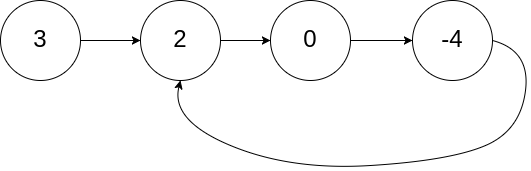
\includegraphics[width=100mm,height=50mm]{images/leetcode/circularlinkedlist.png}

\textbf{示例 2}:

\begin{verbatim}
  输入:head = [1,2], pos = 0
  输出:tail connects to node index 0
  解释:链表中有一个环,其尾部连接到第一个节点。
\end{verbatim}

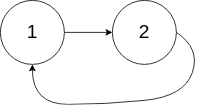
\includegraphics[width=60mm,height=30mm]{images/leetcode/circularlinkedlist_test2.png}

\textbf{示例 3}:

\begin{verbatim}
  输入:head = [1], pos = -1
  输出:no cycle
  解释:链表中没有环。
\end{verbatim}


\includegraphics[width=15mm,height=15mm]{images/leetcode/circularlinkedlist_test3.png}

\textbf{进阶}:\\
你是否可以不用额外空间解决此题?

\subsection{参考题解}

\begin{verbatim}
/**
 * Definition for singly-linked list.
 * function ListNode(val) {
 *     this.val = val;
 *     this.next = null;
 * }
 */
/**
 * @param {ListNode} head
 * @return {ListNode}
 */
var detectCycle = function(head) {
  let ptr1 = getIntersection(head);
  if (ptr1 === null) {
    return null;
  }
  let ptr2 = head;

  while (ptr1 !== ptr2) {
    ptr1 = ptr1.next;
    ptr2 = ptr2.next;
  }
  return ptr1;
};

var getIntersection = function(head) {
  let slow = head;
  let fast = head;
  while (slow && fast && fast.next) {
    slow = slow.next;
    fast = fast.next.next;
    if (slow === fast) {
      return slow;
    }
  }
  return null;
};
\end{verbatim}

\newpage
\section{144. 二叉树的前序遍历}
\label{leetcode:144}

\subsection{题目}

给定一个二叉树,返回它的前序遍历。

\textbf{示例}:

\begin{verbatim}
  输入: [1,null,2,3]  
     1
      \
       2
      /
     3 

  输出: [1,2,3]
\end{verbatim}

\textbf{进阶}: 递归算法很简单,你可以通过迭代算法完成吗?

\subsection{参考题解}

\begin{verbatim}
/**
 * Definition for a binary tree node.
 * function TreeNode(val) {
 *     this.val = val;
 *     this.left = this.right = null;
 * }
 */
/**
 * @param {TreeNode} root
 * @return {number[]}
 */
var preorderTraversal = function(root) {
  let result = [];
  recursion(root, result);
  return result;
};

function recursion(root, result) {
  if (root === null) { return; }
  result.push(root.val);
  recursion(root.left, result);
  recursion(root.right, result);
}
\end{verbatim}

\newpage
\section{152. 乘积最大子序列}
\label{leetcode:152}

\newpage
\section{153. 寻找旋转排序数组中的最小值}
\label{leetcode:153}

\subsection{题目}

假设按照升序排序的数组在预先未知的某个点上进行了旋转。

( 例如,数组 [0,1,2,4,5,6,7] 可能变为 [4,5,6,7,0,1,2] )。

请找出其中最小的元素。

你可以假设数组中不存在重复元素。

\textbf{示例 1}:

\begin{verbatim}
  输入: [3,4,5,1,2]
  输出: 1
\end{verbatim}

\textbf{示例 2}:

\begin{verbatim}
  输入: [4,5,6,7,0,1,2]
  输出: 0
\end{verbatim}

\subsection{参考题解,二分查找}

\begin{verbatim}
/**
 * @param {number[]} nums
 * @return {number}
 */
var findMin = function(nums) {
  let left = 0;
  let right = nums.length - 1;
  while (left < right) {
    let mid = left + Math.floor((right - left) / 2);
    if (nums[mid] > nums[right]) {
      left = mid + 1;
    } else {
      right = mid;
    }
  }
  return nums[left];
};
\end{verbatim}

\newpage
\section{155. 最小栈}
\label{leetcode:155}

\begin{verbatim}
/**
 * initialize your data structure here.
 */
var MinStack = function() {
  this.stack = [];
  this.minstack = [];
};

/**
 * @param {number} x
 * @return {void}
 */
MinStack.prototype.push = function(x) {
  this.stack.push(x);
  if (this.minstack.length === 0) {
    this.minstack.push(x);
  } else {
    if (x <= this.minstack[this.minstack.length - 1]) {
      this.minstack.push(x);
    }
  }
};

/**
 * @return {void}
 */
MinStack.prototype.pop = function() {
  if (this.stack.length === 0) {
    return;
  }
  const x = this.stack.pop();
  if (x === this.minstack[this.minstack.length - 1]) {
    this.minstack.pop();
  }
};

/**
 * @return {number}
 */
MinStack.prototype.top = function() {
  return this.stack[this.stack.length - 1];
};

/**
 * @return {number}
 */
MinStack.prototype.getMin = function() {
  return this.minstack[this.minstack.length - 1];
};

/**
 * Your MinStack object will be instantiated and called as such:
 * var obj = new MinStack()
 * obj.push(x)
 * obj.pop()
 * var param_3 = obj.top()
 * var param_4 = obj.getMin()
 */
\end{verbatim}

\newpage
\section{169. 多数元素}
\label{leetcode:169}

\subsection{题目}

给定一个大小为 n 的数组,找到其中的多数元素。
多数元素是指在数组中出现次数\textbf{大于} ⌊ n/2 ⌋ 的元素。

你可以假设数组是非空的,并且给定的数组总是存在多数元素。

\textbf{示例 1}:

\begin{verbatim}
  输入: [3,2,3]
  输出: 3
\end{verbatim}

\textbf{示例 2}:

\begin{verbatim}
  输入: [2,2,1,1,1,2,2]
  输出: 2
\end{verbatim}

\subsection{参考题解,哈希表}

用哈希表把每个数字出现的次数都记录下来,
然后看下哪个数字出现的次数最多就是我们要的了。

\begin{verbatim}
/**
 * @param {number[]} nums
 * @return {number}
 */
var majorityElement = function(nums) {
  const m = {};
  for (let i = 0; i < nums.length; i += 1) {
    const num = nums[i];
    if (num in m) {
      m[num] += 1;
    } else {
      m[num] = 1;
    }
    if (m[num] > nums.length / 2) {
      return num;
    }
  }
};
\end{verbatim}

\subsection{参考题解,经典题解}

\begin{verbatim}
/**
 * @param {number[]} nums
 * @return {number}
 */
var majorityElement = function(nums) {
  let count = 0;
  let candidate = null;
  for (let i = 0; i < nums.length; i += 1) {
    const num = nums[i];
    if (count === 0) {
      candidate = num;
    }
    count += num === candidate ? 1 : -1;
  }
  return candidate;
};
\end{verbatim}

\newpage
\section{188. 买卖股票的最佳时机 IV}
\label{leetcode:188}

\newpage
\section{189. 旋转数组}
\label{leetcode:189}

\subsection{题目}

给定一个数组,将数组中的元素向右移动 k 个位置,其中 k 是非负数。

\textbf{示例 1}:

\begin{verbatim}
  输入: [1,2,3,4,5,6,7] 和 k = 3
  输出: [5,6,7,1,2,3,4]
  解释:
  向右旋转 1 步: [7,1,2,3,4,5,6]
  向右旋转 2 步: [6,7,1,2,3,4,5]
  向右旋转 3 步: [5,6,7,1,2,3,4]
\end{verbatim}

\textbf{示例 2}:

\begin{verbatim}
  输入: [-1,-100,3,99] 和 k = 2
  输出: [3,99,-1,-100]
  解释: 
  向右旋转 1 步: [99,-1,-100,3]
  向右旋转 2 步: [3,99,-1,-100]
\end{verbatim}

\textbf{说明}:

\begin{enumerate}
  \item 尽可能想出更多的解决方案,至少有三种不同的方法可以解决这个问题。
  \item 要求使用空间复杂度为 O(1) 的\textbf{原地}算法。
\end{enumerate}

\subsection{参考题解}

\begin{verbatim}
/**
 * @param {number[]} nums
 * @param {number} k
 * @return {void} Do not return anything, 
 *   modify nums in-place instead.
 */
var rotate = function(nums, k) {
  k = k % nums.length;
  reverse(nums, 0, nums.length - k - 1);
  reverse(nums, nums.length - k, nums.length - 1);
  reverse(nums, 0, nums.length - 1);
};

function reverse(nums, start, end) {
  while (start < end) {
    [nums[start], nums[end]] = [nums[end], nums[start]];
    start += 1;
    end -= 1;
  }
}
\end{verbatim}

\newpage
\section{198. 打家劫舍}
\label{leetcode:198}

\newpage
\section{200. 岛屿数量}
\label{leetcode:200}

\subsection{题目}

给定一个由 \verb|'1'|(陆地)和 \verb|'0'|(水)组成的的二维网格,计算岛屿的数量。
一个岛被水包围,并且它是通过水平方向或垂直方向上相邻的陆地连接而成的。
你可以假设网格的四个边均被水包围。

\textbf{示例 1}:

\begin{verbatim}
  输入:
  11110
  11010
  11000
  00000

  输出: 1
\end{verbatim}

\textbf{示例 2}:

\begin{verbatim}
  输入:
  11000
  11000
  00100
  00011

  输出: 3
\end{verbatim}

\subsection{参考题解,沉岛模式,BFS}

就是碰到一个 1 就把和这个 1 相连在一起的所有 1 都变成 0。

\subsubsection{JavaScript}

\begin{verbatim}
/**
* @param {character[][]} grid
* @return {number}
*/
var numIslands = function(grid) {
  if (grid.length === 0) { return 0; }
  let rows = grid.length;
  let cols = grid[0].length;
  let count = 0;
  for (let row = 0; row < rows; row += 1) {
    for (let col = 0; col < cols; col += 1) {
      if (grid[row][col] === "1") {
        count += 1;
        destroyIslandBFS(grid, row, col);
      }
    }
  }
  return count;
};

function destroyIslandBFS(grid, row, col) {
  const dirs = [ [-1, 0], [1, 0], [0, -1], [0, 1] ];
  grid[row][col] = "0";
  let queue = [];
  queue.push([row, col]);
  while (queue.length > 0) {
    let cur = queue.shift();
    let curRow = cur[0];
    let curCol = cur[1];
    for (let i = 0; i < dirs.length; i += 1) {
      let newRow = curRow + dirs[i][0];
      let newCol = curCol + dirs[i][1];
      if (isIndexValid(grid, newRow, newCol) &&
        grid[newRow][newCol] === "1") {
        grid[newRow][newCol] = "0";
        queue.push([newRow, newCol]);
      }
    }
  }
}

function isIndexValid(grid, row, col) {
  if (row < 0 ||
      col < 0 ||
      row >= grid.length ||
      col >= grid[0].length) {
    return false;
  }
  return true;
}
\end{verbatim}

\subsubsection{Python}

\begin{verbatim}
class Solution:
  def numIslands(self, grid: List[List[str]]) -> int:
    if len(grid) == 0: return 0
    rows, cols, count = len(grid), len(grid[0]), 0
    for row in range(rows):
      for col in range(cols):
        if grid[row][col] == '1':
          count += 1
          self.destoryIslandBFS(grid, row, col)
    return count

  def destoryIslandBFS(self, grid, row, col):
    rows, cols = len(grid), len(grid[0])
    queue = [(row, col)]
    while queue:
      curRow, curCol = queue.pop(0)
      for x, y in [(-1, 0), (1, 0), (0, -1), (0, 1)]:
        newRow, newCol = curRow + x, curCol + y
        if 0 <= newRow < rows and \
          0 <= newCol < cols and \
          grid[newRow][newCol] == '1':
          grid[newRow][newCol] = '0'
          queue.append((newRow, newCol))
\end{verbatim}

\subsection{参考题解,沉岛模式,DFS}

\begin{verbatim}
/**
 * @param {character[][]} grid
 * @return {number}
 */
var numIslands = function(grid) {
  if (grid.length === 0) { return 0; }
  let rows = grid.length;
  let cols = grid[0].length;
  let count = 0;
  for (let row = 0; row < rows; row += 1) {
    for (let col = 0; col < cols; col += 1) {
      if (grid[row][col] === "1") {
        count += 1;
        destroyIslandDFS(grid, row, col);
      }
    }
  }
  return count;
};

function destroyIslandDFS(grid, row, col) {
  grid[row][col] = "0";
  const dirs = [ [-1, 0], [1, 0], [0, -1], [0, 1] ];
  for (let i = 0; i < dirs.length; i += 1) {
    let newRow = row + dirs[i][0];
    let newCol = col + dirs[i][1];
    if (isIndexValid(grid, newRow, newCol) &&
      grid[newRow][newCol] === "1") {
      destroyIslandDFS(grid, newRow, newCol);
    }
  }
}

function isIndexValid(grid, row, col) {
  if (row < 0 ||
      col < 0 ||
      row >= grid.length ||
      col >= grid[0].length) {
    return false;
  }
  return true;
}
\end{verbatim}

\subsection{参考题解,并查集}

\subsubsection{Python}

\begin{verbatim}
class Solution:
  def numIslands(self, grid: List[List[str]]) -> int:
    if not grid: return 0
    rows = len(grid)
    cols = len(grid[0])
    p = {}
    for row in range(rows):
      for col in range(cols):
        if grid[row][col] == "1":
          p[row * cols + col] = row * cols + col

    directions = [[-1, 0], [1, 0], [0, -1], [0, 1]]
    for row in range(rows):
      for col in range(cols):
        if grid[row][col] == "1":
          for _, dirs in enumerate(directions):
            newRow = row + dirs[0]
            newCol = col + dirs[1]
            if self.isValid(grid, newRow, newCol):
              self.union(p, row * cols + col, newRow * cols + newCol)

    return len(set([self.parent(p, key) for key in p]))

  def isValid(self, grid, row, col):
    if row < 0 or row >= len(grid):
      return False
    if col < 0 or col >= len(grid[0]):
      return False
    if grid[row][col] == "0":
      return False
    return True

  def union(self, p, i, j):
    p1 = self.parent(p, i)
    p2 = self.parent(p, j)
    p[p1] = p2

  def parent(self, p, i):
    root = i
    while p[root] != root:
      root = p[root]
    while p[i] != i:
      x = i
      i = p[i]
      p[x] = root
    return root
\end{verbatim}



\chapter{LeetCode 题目(200-End)}

\newpage
\section{206. 反转链表}
\label{leetcode:206}

\subsection{题目}

反转一个单链表。

\textbf{示例}:

\begin{verbatim}
  输入: 1->2->3->4->5->NULL
  输出: 5->4->3->2->1->NULL
\end{verbatim}

\textbf{进阶}: \\
你可以迭代或递归地反转链表。你能否用两种方法解决这道题?

\subsection{参考题解,迭代}

\begin{verbatim}
/**
 * Definition for singly-linked list.
 * function ListNode(val) {
 *     this.val = val;
 *     this.next = null;
 * }
 */
/**
 * @param {ListNode} head
 * @return {ListNode}
 */
var reverseList = function(head) {
  let [pre, cur] = [null, head];
  while (cur !== null) {
    let next = cur.next;
    cur.next = pre;
    pre = cur;
    cur = next;
  }
  return pre;
};
\end{verbatim}

\subsection{参考题解,递归}

\begin{verbatim}
/**
 * Definition for singly-linked list.
 * function ListNode(val) {
 *     this.val = val;
 *     this.next = null;
 * }
 */
/**
 * @param {ListNode} head
 * @return {ListNode}
 */
var reverseList = function(head) {
  if (head === null || head.next === null) {
    return head;
  }
  let p = reverseList(head.next);
  head.next.next = head;
  head.next = null;
  return p;
};
\end{verbatim}

\newpage
\section{208. 实现 Trie (前缀树)}
\label{leetcode:208}

\newpage
\section{212. 单词搜索 II}
\label{leetcode:212}

\newpage
\section{213. 打家劫舍 II}
\label{leetcode:213}

\newpage
\section{221. 最大正方形}
\label{leetcode:221}

\newpage
\section{226. 翻转二叉树}
\label{leetcode:226}

\subsection{题目}

翻转一棵二叉树。

\textbf{示例}:

\begin{verbatim}
输入:

     4
   /   \
  2     7
 / \   / \
1   3 6   9

输出:

     4
   /   \
  7     2
 / \   / \
9   6 3   1
\end{verbatim}

\subsection{参考题解}

\begin{verbatim}
/**
 * Definition for a binary tree node.
 * function TreeNode(val) {
 *     this.val = val;
 *     this.left = this.right = null;
 * }
 */
/**
 * @param {TreeNode} root
 * @return {TreeNode}
 */
var invertTree = function(root) {
  if (!root) { return root; }
  const left = root.left;
  const right = root.right;
  root.right = invertTree(left);
  root.left = invertTree(right);
  return root;
};
\end{verbatim}

\newpage
\section{236. 二叉树的最近公共祖先}
\label{leetcode:236}

\subsection{题目}

给定一个二叉树, 找到该树中两个指定节点的最近公共祖先。

百度百科中最近公共祖先的定义为:``对于有根树 T 的两个结点 p、q,
最近公共祖先表示为一个结点 x,满足 x 是 p、q 的祖先且 x 的深度尽可能大
(一个节点也可以是它自己的祖先)。''

例如,给定如下二叉树:  root = [3,5,1,6,2,0,8,null,null,7,4]

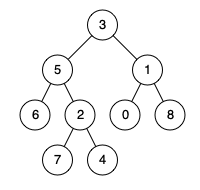
\includegraphics[width=60mm,height=60mm]{images/leetcode/leetcode_236_binarytree.png}

\textbf{示例 1}:

\begin{verbatim}
  输入: root = [3,5,1,6,2,0,8,null,null,7,4], p = 5, q = 1
  输出: 3
  解释: 节点 5 和节点 1 的最近公共祖先是节点 3。
\end{verbatim}

\textbf{示例 2}:

\begin{verbatim}
  输入: root = [3,5,1,6,2,0,8,null,null,7,4], p = 5, q = 4
  输出: 5
  解释: 节点 5 和节点 4 的最近公共祖先是节点 5。
  因为根据定义最近公共祖先节点可以为节点本身。
\end{verbatim}

\textbf{说明}:

\begin{enumerate}
  \item 所有节点的值都是唯一的。
  \item p、q 为不同节点且均存在于给定的二叉树中。
\end{enumerate}

\subsection{参考题解}

\begin{verbatim}
/**
 * Definition for a binary tree node.
 * function TreeNode(val) {
 *     this.val = val;
 *     this.left = this.right = null;
 * }
 */
/**
 * @param {TreeNode} root
 * @param {TreeNode} p
 * @param {TreeNode} q
 * @return {TreeNode}
 */
var lowestCommonAncestor = function(root, p, q) {
  if (root === null || root === p || root === q) {
    return root;
  }
  let left = lowestCommonAncestor(root.left, p, q);
  let right = lowestCommonAncestor(root.right, p, q);
  if (left === null) { return right; }
  if (right === null) { return left; }
  return root;
};
\end{verbatim}

\newpage
\section{239. 滑动窗口最大值}
\label{leetcode:239}

\subsection{题目}

给定一个数组 nums,有一个大小为 k 的滑动窗口从数组的最左侧移动到数组的最右侧。
你只可以看到在滑动窗口内的 k 个数字。滑动窗口每次只向右移动一位。

返回滑动窗口中的最大值。

\textbf{示例}:

\begin{verbatim}
输入: nums = [1,3,-1,-3,5,3,6,7], 和 k = 3
输出: [3,3,5,5,6,7] 
解释: 

  滑动窗口的位置                最大值
---------------               -----
[1  3  -1] -3  5  3  6  7       3
 1 [3  -1  -3] 5  3  6  7       3
 1  3 [-1  -3  5] 3  6  7       5
 1  3  -1 [-3  5  3] 6  7       5
 1  3  -1  -3 [5  3  6] 7       6
 1  3  -1  -3  5 [3  6  7]      7
\end{verbatim}

\textbf{提示}:\\
你可以假设 k 总是有效的,在输入数组不为空的情况下,1 $\leq$ k $\leq$ 输入数组的大小。

\textbf{进阶}:\\
你能在线性时间复杂度内解决此题吗?

\subsection{参考题解}

\begin{verbatim}
/**
 * @param {number[]} nums
 * @param {number} k
 * @return {number[]}
 */
var maxSlidingWindow = function(nums, k) {
  if (nums.length === 0) { return []; }
  let result = [];
  let window = [];
  for (let i = 0; i < nums.length; i += 1) {
    if (i >= k && window[0] <= i - k) {
      window.shift();
    }
    while (window.length > 0 && nums[window[window.length - 1]] <= nums[i]) {
      window.pop();
    }
    window.push(i);
    if (i >= k - 1) {
      result.push(nums[window[0]]);
    }
  }
  return result;
};
\end{verbatim}

\newpage
\section{242. 有效的字母异位词} 
\label{leetcode:242}

\subsection{题目}

给定两个字符串 s 和 t ,编写一个函数来判断 t 是否是 s 的字母异位词。

\textbf{示例 1}:

\begin{verbatim}
  输入: s = "anagram", t = "nagaram"
  输出: true
\end{verbatim}

\textbf{示例 2}:

\begin{verbatim}
  输入: s = "rat", t = "car"
  输出: false
\end{verbatim}

\textbf{说明}:\\
你可以假设字符串只包含小写字母。

\textbf{进阶}:\\
如果输入字符串包含 unicode 字符怎么办?你能否调整你的解法来应对这种情况?

\subsection{参考题解}

\begin{verbatim}
/**
 * @param {string} s
 * @param {string} t
 * @return {boolean}
 */
var isAnagram = function(s, t) {
  if (s.length !== t.length) { return false; }
  const m = new Array(26).fill(0);
  for (let i = 0; i < s.length; i += 1) {
    m[s.charCodeAt(i) - 97]++;
    m[t.charCodeAt(i) - 97]--;
  }
  return m.filter(e => e > 0).length === 0;
};
\end{verbatim}

\newpage
\section{279. 完全平方数}
\label{leetcode:279}

\newpage
\section{283. 移动零}
\label{leetcode:283}

\begin{verbatim}
/**
 * @param {number[]} nums
 * @return {void} Do not return anything, 
 *   modify nums in-place instead.
 */
var moveZeroes = function(nums) {
  let j = 0;
  for (let i = 0; i < nums.length; i += 1) {
    if (nums[i] !== 0) {
      [nums[i], nums[j]] = [nums[j], nums[i]];
      j += 1;
    }
  }
};
\end{verbatim}

\newpage
\section{297. 二叉树的序列化与反序列化}
\label{leetcode:297}

\begin{verbatim}
/**
 * Definition for a binary tree node.
 * function TreeNode(val) {
 *     this.val = val;
 *     this.left = this.right = null;
 * }
 */

/**
 * Encodes a tree to a single string.
 *
 * @param {TreeNode} root
 * @return {string}
 */
var serialize = function(root) {
  let result = [];
  serializeDFS(root, result);
  return result.join(",");
};

function serializeDFS(root, result) {
  if (root === null) {
    result.push("null");
    return;
  }
  result.push(root.val);
  serializeDFS(root.left, result);
  serializeDFS(root.right, result);
}

/**
 * Decodes your encoded data to tree.
 *
 * @param {string} data
 * @return {TreeNode}
 */
var deserialize = function(data) {
  let array = data.split(",");
  return deserializeRecursion(array);
};

function deserializeRecursion(array) {
  if (array.length === 0) { return null; }

  let val = array[0];
  if (val === 'null') {
    array.shift();
    return null;
  }

  let node = new TreeNode(+val);
  array.shift();
  node.left = deserializeRecursion(array);
  node.right = deserializeRecursion(array);
  return node;
}

/**
 * Your functions will be called as such:
 * deserialize(serialize(root));
 */
\end{verbatim}

\newpage
\section{309. 最佳买卖股票时机含冷冻期}
\label{leetcode:309}

\newpage
\section{312. 戳气球}
\label{leetcode:312}

\newpage
\section{322. 零钱兑换}
\label{leetcode:322}

\newpage
\section{338. 比特位计数}
\label{leetcode:338}

\subsection{题目}

\newpage
\section{344. 反转字符串}
\label{leetcode:344}

\subsection{题目}

\newpage
\section{363. 矩形区域不超过 K 的最大数值和}
\label{leetcode:363}

\newpage
\section{367. 有效的完全平方数}
\label{leetcode:367}

\subsection{题目}

给定一个正整数 num,编写一个函数,如果 num 是一个完全平方数,则返回 True,否则返回 False。

说明:不要使用任何内置的库函数,如  sqrt。

\textbf{示例 1}:

\begin{verbatim}
  输入:16
  输出:True
\end{verbatim}

\textbf{示例 2}:

\begin{verbatim}
  输入:14
  输出:False
\end{verbatim}

\subsection{参考题解,二分法}

\subsubsection{Java}

\begin{verbatim}
class Solution {
  public boolean isPerfectSquare(int num) {
    if (num < 2) {
      return true;
    }
    long left = 0;
    long right = num / 2;
    while (left <= right) {
      long mid = left + (right - left) / 2;
      long guessed = mid * mid;
      if (guessed == num) {
        return true;
      } else if (guessed > num) {
        right = mid - 1;
      } else {
        left = mid + 1;
      }
    }
    return false;
  }
}
\end{verbatim}

\subsubsection{JavaScript}

\begin{verbatim}
/**
 * @param {number} num
 * @return {boolean}
 */
var isPerfectSquare = function(num) {
  if (num < 2) { return true; }
  let left = 2;
  let right = Math.floor(num / 2);
  while (left <= right) {
    let mid = left + Math.floor((right - left) / 2);
    let guessSquared = mid * mid;
    if (guessSquared === num) {
      return true;
    } else if (guessSquared < num) {
      left = mid + 1;
    } else {
      right = mid - 1;
    }
  }
  return false;
};
\end{verbatim}

\newpage
\section{387. 字符串中的第一个唯一字符}
\label{leetcode:387}

\subsection{题目}


\newpage
\section{429. N叉树的层序遍历}
\label{leetcode:429}

\begin{verbatim}
/**
 * // Definition for a Node.
 * function Node(val,children) {
 *    this.val = val;
 *    this.children = children;
 * };
 */
/**
 * @param {Node} root
 * @return {number[][]}
 */
var levelOrder = function(root) {
  if (root === null) { return []; }
  let result = [];
  let queue = [];
  queue.push(root);
  while (queue.length > 0) {
    let currentLevel = queue;
    queue = [];
    for (let i = 0; i < currentLevel.length; i += 1) {
      let currNode = currentLevel[i];
      for (let j = 0; j < currNode.children.length; j += 1) {
        queue.push(currNode.children[j]);
      }
    }
    result.push(currentLevel.map(e => e.val));
  }
  return result;
};
\end{verbatim}
\newpage
\section{433. 最小基因变化}
\label{leetcode:433}

\subsection{题目}

一条基因序列由一个带有8个字符的字符串表示,其中每个字符都属于 
``A'', ``C'', ``G'', ``T''中的任意一个。

假设我们要调查一个基因序列的变化。一次基因变化意味着这个基因序列中的一个字符发生了变化。

例如,基因序列由 ``AACCGGTT'' 变化至 ``AACCGGTA'' 即发生了一次基因变化。

与此同时,每一次基因变化的结果,都需要是一个合法的基因串,即该结果属于一个基因库。

现在给定3个参数 — start, end, bank,分别代表起始基因序列,目标基因序列及基因库,
请找出能够使起始基因序列变化为目标基因序列所需的最少变化次数。
如果无法实现目标变化,请返回 -1。

\textbf{注意}:

\begin{itemize}
  \item 起始基因序列默认是合法的,但是它并不一定会出现在基因库中。
  \item 所有的目标基因序列必须是合法的。
  \item 假定起始基因序列与目标基因序列是不一样的。
\end{itemize}

\textbf{示例 1}:

\begin{verbatim}
  start: "AACCGGTT"
  end:   "AACCGGTA"
  bank: ["AACCGGTA"]

  返回值: 1
\end{verbatim}

\textbf{示例 2}:

\begin{verbatim}
  start: "AACCGGTT"
  end:   "AAACGGTA"
  bank: ["AACCGGTA", "AACCGCTA", "AAACGGTA"]

  返回值: 2
\end{verbatim}

\textbf{示例 3}:

\begin{verbatim}
  start: "AAAAACCC"
  end:   "AACCCCCC"
  bank: ["AAAACCCC", "AAACCCCC", "AACCCCCC"]

  返回值: 3
\end{verbatim}

\subsection{参考题解,暴力法}

\begin{verbatim}
/**
 * @param {string} start
 * @param {string} end
 * @param {string[]} bank
 * @return {number}
 */
var minMutation = function(start, end, bank) {
  if (start === end) { return 0; }
  const charSet = ['A', 'C', 'G', 'T'];
  const bankSet = new Set(bank);
  let level = 0;
  const queue = [];
  const visited = new Set();
  queue.push(start);
  visited.add(start);
  while (queue.length > 0) {
    let levelSize = queue.length;
    while (levelSize-- > 0) {
      let cur = queue.shift();
      if (cur === end) {
        return level;
      }
      let curCharArray = cur.split("");
      for (let i = 0; i < curCharArray.length; i += 1) {
        let old = curCharArray[i];
        for (let j = 0; j < charSet.length; j += 1) {
          curCharArray[i] = charSet[j];
          let next = curCharArray.join("");
          if (!visited.has(next) && bankSet.has(next)) {
            visited.add(next);
            queue.push(next);
          }
        }
        curCharArray[i] = old;
      }
    }
    level += 1;
  }
  return -1;
};
\end{verbatim}

\newpage
\section{455. 分发饼干}
\label{leetcode:455}

\subsection{题目}

假设你是一位很棒的家长,想要给你的孩子们一些小饼干。
但是,每个孩子最多只能给一块饼干。对每个孩子 i ,都有一个胃口值 $g_{i}$ ,
这是能让孩子们满足胃口的饼干的最小尺寸;并且每块饼干 j ,都有一个尺寸 $s_{j}$ 。
如果 $s_{j}$ >= $g_{i}$ ,我们可以将这个饼干 j 分配给孩子 i ,这个孩子会得到满足。
你的目标是尽可能满足越多数量的孩子,并输出这个最大数值。

\textbf{注意}:

你可以假设胃口值为正。\\
一个小朋友最多只能拥有一块饼干。

\textbf{示例 1}:

\begin{verbatim}
  输入: [1,2,3], [1,1]

  输出: 1

  解释: 
  你有三个孩子和两块小饼干,3个孩子的胃口值分别是:1,2,3。
  虽然你有两块小饼干,由于他们的尺寸都是1,
  你只能让胃口值是1的孩子满足。
  所以你应该输出1。
\end{verbatim}

\textbf{示例 2}:

\begin{verbatim}
  输入: [1,2], [1,2,3]

  输出: 2

  解释: 
  你有两个孩子和三块小饼干,2个孩子的胃口值分别是1,2。
  你拥有的饼干数量和尺寸都足以让所有孩子满足。
  所以你应该输出2.
\end{verbatim}

\subsection{参考题解}

对于每个孩子,都尽量用能够满足他的最小的饼干。

\begin{verbatim}
/**
 * @param {number[]} g
 * @param {number[]} s
 * @return {number}
 */
var findContentChildren = function(g, s) {
  if (g === null || s === null) {
    return 0;
  }
  g.sort((a, b) => a - b);
  s.sort((a, b) => a - b);
  let gi = 0;
  let si = 0;
  while (gi < g.length && si < s.length) {
    if (g[gi] <= s[si]) {
      gi += 1;
    }
    si += 1;
  }
  return gi;
};
\end{verbatim}


\newpage
\section{509. 斐波那契数}
\label{leetcode:509}

\newpage
\section{515. 在每个树行中找最大值}
\label{leetcode:515}

\subsection{题目}

您需要在二叉树的每一行中找到最大的值。

\textbf{示例}:

\begin{verbatim}
  输入: 

          1
         / \
        3   2
       / \   \  
      5   3   9 

  输出: [1, 3, 9]
\end{verbatim}

\subsection{参考题解,BFS}

\begin{verbatim}
/**
 * Definition for a binary tree node.
 * function TreeNode(val) {
 *     this.val = val;
 *     this.left = this.right = null;
 * }
 */
/**
 * @param {TreeNode} root
 * @return {number[]}
 */
var largestValues = function(root) {
  if (root === null || root.length === 0) {
    return [];
  }
  let result = [];
  let queue = [];
  queue.push(root);
  while (queue.length > 0) {
    const currentLevel = queue;
    queue = [];

    let curMax = currentLevel[0];
    for (let i = 1; i < currentLevel.length; i += 1) {
      if (currentLevel[i].val > curMax.val) {
        curMax = currentLevel[i]
      }
    }
    result.push(curMax.val);

    for (let i = 0; i < currentLevel.length; i += 1) {
      const node = currentLevel[i];
      if (node.left) { queue.push(node.left); }
      if (node.right) { queue.push(node.right); }
    }
  }
  return result;
};
\end{verbatim}

\newpage
\section{518. 零钱兑换 II}
\label{leetcode:518}

\subsection{题目}

给定不同面额的硬币和一个总金额。写出函数来计算可以凑成总金额的硬币组合数。假设每一种面额的硬币有无限个。 

\textbf{示例 1}:

\begin{verbatim}
  输入: amount = 5, coins = [1, 2, 5]
  输出: 4
  解释: 有四种方式可以凑成总金额:
  5=5
  5=2+2+1
  5=2+1+1+1
  5=1+1+1+1+1
\end{verbatim}

\textbf{示例 2}:

\begin{verbatim}
  输入: amount = 3, coins = [2]
  输出: 0
  解释: 只用面额2的硬币不能凑成总金额3。
\end{verbatim}

\textbf{示例 3}:

\begin{verbatim}
  输入: amount = 10, coins = [10]
  输出: 1
\end{verbatim}

\textbf{注意}:

你可以假设:

\begin{verbatim}
  0 <= amount (总金额) <= 5000
  1 <= coin (硬币面额) <= 5000
  硬币种类不超过 500 种
  结果符合 32 位符号整数
\end{verbatim}

\subsection{参考题解,动态规划}

\begin{verbatim}
class Solution:
  def change(self, amount: int, coins: List[int]) -> int:
    dp = [1] + [0 for _ in range(amount)]
    for coin in coins:
      for col in range(coin, amount + 1):
        dp[col] += dp[col - coin]
    return dp[-1]
\end{verbatim}

\newpage
\section{529. 扫雷游戏}
\label{leetcode:529}

\subsection{题目}

让我们一起来玩扫雷游戏!

给定一个代表游戏板的二维字符矩阵。'M' 代表一个未挖出的地雷,
'E' 代表一个未挖出的空方块,'B' 代表没有相邻(上,下,左,右,和所有4个对角线)
地雷的已挖出的空白方块,数字('1' 到 '8')表示有多少地雷与这块已挖出的方块相邻,
'X' 则表示一个\textbf{已挖出的}地雷。

现在给出在所有\textbf{未挖出的}方块中('M'或者'E')的下一个点击位置(行和列索引),
根据以下规则,返回相应位置被点击后对应的面板:

\begin{itemize}
  \item 如果一个地雷('M')被挖出,游戏就结束了- 把它改为 'X'。
  \item 如果一个\textbf{没有相邻地雷}的空方块('E')被挖出,修改它为('B'),
    并且所有和其相邻的方块都应该被递归地揭露。
  \item 如果一个至少与一个地雷相邻的空方块('E')被挖出,
    修改它为数字('1'到'8'),表示相邻地雷的数量。
  \item 如果在此次点击中,若无更多方块可被揭露,则返回面板。
\end{itemize}

\textbf{示例 1}:

\begin{verbatim}
  输入: 

  [['E', 'E', 'E', 'E', 'E'],
  ['E', 'E', 'M', 'E', 'E'],
  ['E', 'E', 'E', 'E', 'E'],
  ['E', 'E', 'E', 'E', 'E']]

  Click : [3,0]

  输出: 

  [['B', '1', 'E', '1', 'B'],
  ['B', '1', 'M', '1', 'B'],
  ['B', '1', '1', '1', 'B'],
  ['B', 'B', 'B', 'B', 'B']]
\end{verbatim}

解释:

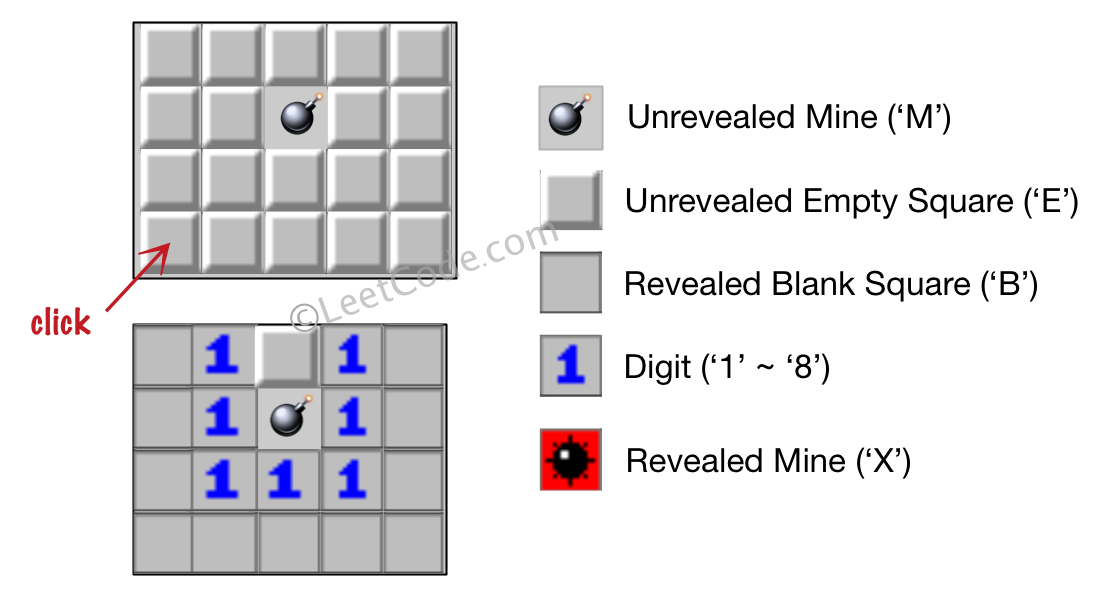
\includegraphics[width=150mm,height=100mm]{images/leetcode/minesweeper_example_1.png}

\textbf{示例 2}:

\begin{verbatim}
  输入: 

  [['B', '1', 'E', '1', 'B'],
  ['B', '1', 'M', '1', 'B'],
  ['B', '1', '1', '1', 'B'],
  ['B', 'B', 'B', 'B', 'B']]

  Click : [1,2]

  输出: 

  [['B', '1', 'E', '1', 'B'],
  ['B', '1', 'X', '1', 'B'],
  ['B', '1', '1', '1', 'B'],
  ['B', 'B', 'B', 'B', 'B']]
\end{verbatim}

解释:

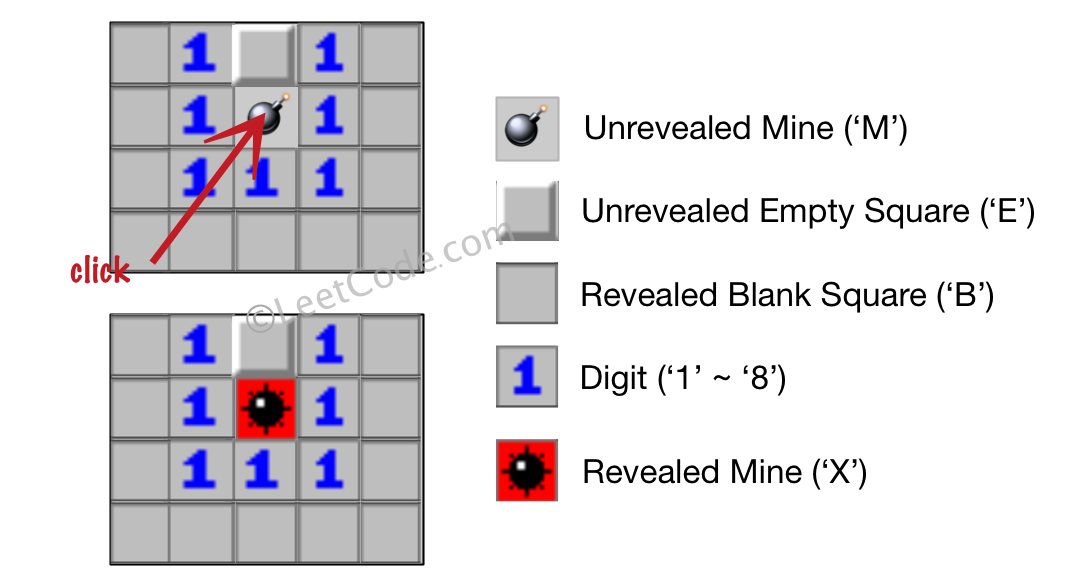
\includegraphics[width=150mm,height=100mm]{images/leetcode/minesweeper_example_2.png}

注意:

\begin{itemize}
  \item 输入矩阵的宽和高的范围为 [1,50]。
  \item 点击的位置只能是未被挖出的方块 ('M' 或者 'E'),
    这也意味着面板至少包含一个可点击的方块。
  \item 输入面板不会是游戏结束的状态(即有地雷已被挖出)。
  \item 简单起见,未提及的规则在这个问题中可被忽略。
    例如,当游戏结束时你不需要挖出所有地雷,考虑所有你可能赢得游戏或标记方块的情况。
\end{itemize}

\subsection{参考题解}

\begin{verbatim}
/**
 * @param {character[][]} board
 * @param {number[]} click
 * @return {character[][]}
 */
var updateBoard = function(board, click) {
  let queue = [];
  queue.push(click);
  while (queue.length > 0) {
    let curClick = queue.shift();
    let curRow = curClick[0];
    let curCol = curClick[1];
    if (board[curRow][curCol] === 'M') {
      board[curRow][curCol] = 'X';
      break;
    } else if (board[curRow][curCol] === 'E') {
      let mineCount = findAdjoinMine(board, curRow, curCol);
      if (mineCount === 0) {
        board[curRow][curCol] = 'B';
        let ms = getAdjoinE(board, curRow, curCol);
        for (let i = 0; i < ms.length; i += 1) {
          queue.push(ms[i]);
        }
      } else {
        board[curRow][curCol] = '' + mineCount;
      }
    }
  }
  return board;
};

const dirs = [
  [-1, 0],
  [1, 0],
  [0, -1],
  [0, 1],
  [-1, -1],
  [1, 1],
  [-1, 1],
  [1, -1],
];

function getAdjoinE(board, row, col) {
  let result = [];
  for (let i = 0; i < dirs.length; i += 1) {
    const newRow = row + dirs[i][0];
    const newCol = col + dirs[i][1];
    if (isValidIndex(board, newRow, newCol)) {
      if (board[newRow][newCol] === 'E') {
        result.push([newRow, newCol]);
      }
    }
  }
  return result;
}

function findAdjoinMine(board, row, col) {
  let count = 0;
  for (let i = 0; i < dirs.length; i += 1) {
    const newRow = row + dirs[i][0];
    const newCol = col + dirs[i][1];
    if (isValidIndex(board, newRow, newCol)) {
      if (board[newRow][newCol] === 'M') {
        count += 1;
      }
    }
  }
  return count;
}

function isValidIndex(board, row, col) {
  if (row < 0 || col < 0) {
    return false;
  }
  if (row >= board.length) {
    return false;
  }
  if (col >= board[0].length) {
    return false;
  }
  return true;
}
\end{verbatim}
\newpage
\section{552. 学生出勤记录 II}
\label{leetcode:552}

\newpage
\section{589. N叉树的前序遍历}
\label{leetcode:589}

\subsection{题目}

给定一个 N 叉树,返回其节点值的前序遍历。

例如,给定一个 3叉树 :

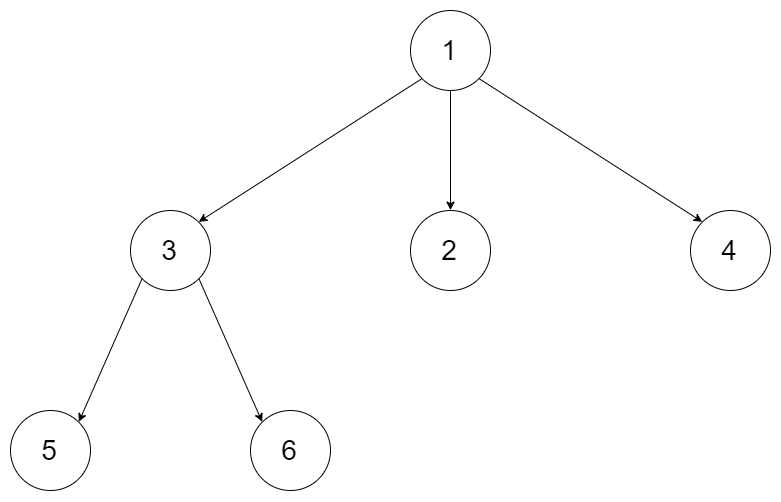
\includegraphics[width=70mm,height=50mm]{images/leetcode/leetcode_429_narytreeexample.png}

返回其前序遍历: [1,3,5,6,2,4]。

说明: 递归法很简单,你可以使用迭代法完成此题吗?

\subsection{参考题解}

\begin{verbatim}
/**
 * // Definition for a Node.
 * function Node(val, children) {
 *    this.val = val;
 *    this.children = children;
 * };
 */
/**
 * @param {Node} root
 * @return {number[]}
 */
var preorder = function(root) {
  let result = [];
  recursion(root, result);
  return result;
};

function recursion(root, result) {
  if (root === null) {
    return;
  }
  result.push(root.val);
  for (let i = 0; i < root.children.length; i += 1) {
    recursion(root.children[i], result);
  }
}
\end{verbatim}

\newpage
\section{590. N叉树的后序遍历}
\label{leetcode:590}

\subsection{题目}

给定一个 N 叉树,返回其节点值的后序遍历。

例如,给定一个 3叉树 :

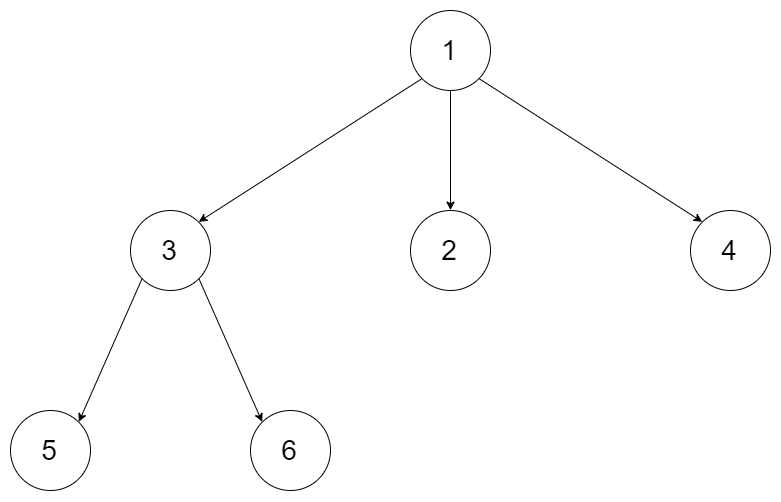
\includegraphics[width=70mm,height=50mm]{images/leetcode/leetcode_429_narytreeexample.png}

返回其后序遍历: [5,6,3,2,4,1]。

说明: 递归法很简单,你可以使用迭代法完成此题吗?

\subsection{参考题解}

\begin{verbatim}
/**
 * // Definition for a Node.
 * function Node(val,children) {
 *    this.val = val;
 *    this.children = children;
 * };
 */
/**
 * @param {Node} root
 * @return {number[]}
 */
var postorder = function(root) {
  let result = [];
  recursion(root, result);
  return result;
};

function recursion(root, result) {
  if (root === null) { return; }
  for (let i = 0; i < root.children.length; i += 1) {
    recursion(root.children[i], result);
  }
  result.push(root.val);
}
\end{verbatim}

\newpage
\section{621. 任务调度器}
\label{leetcode:621}

\newpage
\section{641. 设计循环双端队列}
\label{leetcode:641}

\subsection{题目}

设计实现双端队列。\\
你的实现需要支持以下操作:

\begin{enumerate}
  \item MyCircularDeque(k):构造函数,双端队列的大小为k。
  \item insertFront():将一个元素添加到双端队列头部。 如果操作成功返回 true。
  \item insertLast():将一个元素添加到双端队列尾部。如果操作成功返回 true。
  \item deleteFront():从双端队列头部删除一个元素。 如果操作成功返回 true。
  \item deleteLast():从双端队列尾部删除一个元素。如果操作成功返回 true。
  \item getFront():从双端队列头部获得一个元素。如果双端队列为空,返回 -1。
  \item getRear():获得双端队列的最后一个元素。 如果双端队列为空,返回 -1。
  \item isEmpty():检查双端队列是否为空。
  \item isFull():检查双端队列是否满了。
\end{enumerate}

\textbf{示例}:

\begin{verbatim}
  MyCircularDeque circularDeque = new MycircularDeque(3); // 设置容量大小为3
  circularDeque.insertLast(1);			        // 返回 true
  circularDeque.insertLast(2);			        // 返回 true
  circularDeque.insertFront(3);			        // 返回 true
  circularDeque.insertFront(4);			        // 已经满了,返回 false
  circularDeque.getRear();  				// 返回 2
  circularDeque.isFull();				        // 返回 true
  circularDeque.deleteLast();			        // 返回 true
  circularDeque.insertFront(4);			        // 返回 true
  circularDeque.getFront();				// 返回 4
\end{verbatim}

\textbf{提示}:

\begin{enumerate}
  \item 所有值的范围为 [1, 1000]
  \item 操作次数的范围为 [1, 1000]
  \item 请不要使用内置的双端队列库。
\end{enumerate}

\subsection{参考题解}

\begin{verbatim}
/**
 * Initialize your data structure here. 
 * Set the size of the deque to be k.
 * @param {number} k
 */
var MyCircularDeque = function(k) {
  this.array = new Array(k);
  this.head = 0;
  this.rear = 0;
  this.len = 0;
  this.capacity = k;
};

/**
 * Adds an item at the front of Deque. 
 * Return true if the operation is successful.
 * @param {number} value
 * @return {boolean}
 */
MyCircularDeque.prototype.insertFront = function(value) {
  if (this.isFull()) {
    return false;
  }
  this.array[this.head] = value;
  this.head = (this.head + 1) % this.capacity;
  this.len += 1;
  return true;
};

/**
 * Adds an item at the rear of Deque. 
 * Return true if the operation is successful.
 * @param {number} value
 * @return {boolean}
 */
MyCircularDeque.prototype.insertLast = function(value) {
  if (this.isFull()) {
    return false;
  }
  if (this.rear === 0) {
    this.rear = this.capacity - 1;
  } else {
    this.rear -= 1;
  }
  this.array[this.rear] = value;
  this.len += 1;
  return true;
};

/**
 * Deletes an item from the front of Deque. 
 * Return true if the operation is successful.
 * @return {boolean}
 */
MyCircularDeque.prototype.deleteFront = function() {
  if (this.isEmpty()) {
    return false;
  }
  if (this.head === 0) {
    this.head = this.capacity - 1;
  } else {
    this.head -= 1;
  }
  this.len -= 1;
  return true;
};

/**
 * Deletes an item from the rear of Deque. 
 * Return true if the operation is successful.
 * @return {boolean}
 */
MyCircularDeque.prototype.deleteLast = function() {
  if (this.isEmpty()) {
    return false;
  }
  this.rear = (this.rear + 1) % this.capacity;
  this.len -= 1;
  return true;
};

/**
 * Get the front item from the deque.
 * @return {number}
 */
MyCircularDeque.prototype.getFront = function() {
  if (this.isEmpty()) {
    return -1;
  }
  let prev = this.head === 0 ? this.capacity - 1 : this.head - 1;
  return this.array[prev];
};

/**
 * Get the last item from the deque.
 * @return {number}
 */
MyCircularDeque.prototype.getRear = function() {
  if (this.isEmpty()) {
    return -1;
  }
  return this.array[this.rear];
};

/**
 * Checks whether the circular deque is empty or not.
 * @return {boolean}
 */
MyCircularDeque.prototype.isEmpty = function() {
  return this.len === 0;
};

/**
 * Checks whether the circular deque is full or not.
 * @return {boolean}
 */
MyCircularDeque.prototype.isFull = function() {
  return this.len === this.capacity;
};

/**
 * Your MyCircularDeque object will be instantiated and called as such:
 * var obj = new MyCircularDeque(k)
 * var param_1 = obj.insertFront(value)
 * var param_2 = obj.insertLast(value)
 * var param_3 = obj.deleteFront()
 * var param_4 = obj.deleteLast()
 * var param_5 = obj.getFront()
 * var param_6 = obj.getRear()
 * var param_7 = obj.isEmpty()
 * var param_8 = obj.isFull()
 */
\end{verbatim}

\newpage
\section{647. 回文子串}
\label{leetcode:647}

\newpage
\section{680. 验证回文字符串 Ⅱ}
\label{leetcode:680}

\subsection{题目}

给定一个非空字符串 s,\textbf{最多}删除一个字符。判断是否能成为回文字符串。

\textbf{示例 1}:

\begin{verbatim}
  输入: "aba"
  输出: True
\end{verbatim}

\textbf{示例 2}:

\begin{verbatim}
  输入: "abca"
  输出: True
  解释: 你可以删除c字符。
\end{verbatim}

\textbf{注意}:

字符串只包含从 a-z 的小写字母。字符串的最大长度是50000。

\subsection{参考题解,傻递归}

\subsubsection{Python}

\begin{verbatim}
class Solution:
  def validPalindrome(self, s: str) -> bool:
    def dfs(left, right, canRemove):
      if left >= right:
        return True
      if s[left] == s[right]:
        return dfs(left + 1, right - 1, canRemove)
      elif canRemove:
        return dfs(left + 1, right, False) or dfs(left, right - 1, False)
      else:
        return False
    return dfs(0, len(s) - 1, True)
\end{verbatim}

\subsection{参考题解}

\subsubsection{Python}

\begin{verbatim}
class Solution:
  def validPalindrome(self, s: str) -> bool:
    if s == s[::-1]: return True
    left, right = 0, len(s) - 1
    while left < right:
      if s[left] != s[right]:
        return s[left:right] == s[left:right][::-1] or \
          s[left + 1:right + 1] == s[left + 1:right + 1][::-1]
      left, right = left + 1, right - 1
    return True
\end{verbatim}


\newpage
\section{709. 转换成小写字母}
\label{leetcode:709}

\subsection{题目}

实现函数 ToLowerCase(),该函数接收一个字符串参数 str,
并将该字符串中的大写字母转换成小写字母,之后返回新的字符串。

\textbf{示例 1}:

\begin{verbatim}
  输入: "Hello"
  输出: "hello"
\end{verbatim}

\textbf{示例 2}:

\begin{verbatim}
  输入: "here"
  输出: "here"
\end{verbatim}

\textbf{示例 3}:

\begin{verbatim}
  输入: "LOVELY"
  输出: "lovely"
\end{verbatim}

\subsection{参考题解}

\subsubsection{Python}

\begin{verbatim}
class Solution:
  def toLowerCase(self, str: str) -> str:
    return str.lower()
\end{verbatim}

\newpage
\section{714. 买卖股票的最佳时机含手续费}
\label{leetcode:714}

\subsection{参考题解,动态规划}

每次交易要付手续费,只要把手续费从利润中减去即可。

\begin{verbatim}
  dp[i][0] = max(dp[i-1][0], dp[i-1][1] + prices[i])
  dp[i][1] = max(dp[i-1][1], dp[i-1][0] - prices[i] - fee)
\end{verbatim}

相当于买入股票的价格升高了。

在第一个式子里减也是一样的,相当于卖出股票的价格减少了。

\subsubsection{Python}

\begin{verbatim}
class Solution:
  def maxProfit(self, prices: List[int], fee: int) -> int:
    dp_i_0, dp_i_1 = 0, float('-inf')
    for i in range(len(prices)):
      pre_i_0, pre_i_1 = dp_i_0, dp_i_1
      dp_i_0 = max(pre_i_0, pre_i_1 + prices[i])
      dp_i_1 = max(pre_i_1, pre_i_0 - prices[i] - fee)
    return dp_i_0
\end{verbatim}

\newpage
\section{746. 使用最小花费爬楼梯}
\label{leetcode:746}

\subsection{题目}

\newpage
\section{771. 宝石与石头}
\label{leetcode:771}

\subsection{题目}

给定字符串J 代表石头中宝石的类型,和字符串 S代表你拥有的石头。 
S 中每个字符代表了一种你拥有的石头的类型,你想知道你拥有的石头中有多少是宝石。

J 中的字母不重复,J 和 S中的所有字符都是字母。字母区分大小写,因此``a''和``A''是不同类型的石头。

\textbf{示例 1}:

\begin{verbatim}
  输入: J = "aA", S = "aAAbbbb"
  输出: 3
\end{verbatim}

\textbf{示例 2}:

\begin{verbatim}
  输入: J = "z", S = "ZZ"
  输出: 0
\end{verbatim}

\textbf{注意}:

S 和 J 最多含有50个字母。J 中的字符不重复。

\subsection{参考题解}

\subsubsection{Python}

\begin{verbatim}
class Solution:
  def numJewelsInStones(self, J: str, S: str) -> int:
    Jset = set(J)
    return sum(c in Jset for c in S)
\end{verbatim}

\newpage
\section{773. 滑动谜题}
\label{leetcode:773}


\newpage
\section{818. 赛车}
\label{leetcode:818}

\subsection{题目}

\newpage
\section{860. 柠檬水找零}
\label{leetcode:860}

\newpage
\section{874. 模拟行走机器人}
\label{leetcode:874}

\subsection{题目}

机器人在一个无限大小的网格上行走,从点 (0, 0) 处开始出发,面向北方。
该机器人可以接收以下三种类型的命令:

\begin{enumerate}
  \item -2:向左转 90 度
  \item -1:向右转 90 度
  \item 1 <= x <= 9:向前移动 x 个单位长度
\end{enumerate}

在网格上有一些格子被视为障碍物。

第 i 个障碍物位于网格点  (obstacles[i][0], obstacles[i][1])

如果机器人试图走到障碍物上方,那么它将停留在障碍物的前一个网格方块上,
但仍然可以继续该路线的其余部分。

返回从原点到机器人的最大欧式距离的\textbf{平方}。

\textbf{示例 1}:

\begin{verbatim}
  输入: commands = [4,-1,3], obstacles = []
  输出: 25
  解释: 机器人将会到达 (3, 4)
\end{verbatim}

\textbf{示例 2}:

\begin{verbatim}
  输入: commands = [4,-1,4,-2,4], obstacles = [[2,4]]
  输出: 65
  解释: 机器人在左转走到 (1, 8) 之前将被困在 (1, 4) 处
\end{verbatim}

\textbf{提示}:

\begin{itemize}
  \item 0 <= commands.length <= 10000
  \item 0 <= obstacles.length <= 10000
  \item -30000 <= obstacle[i][0] <= 30000
  \item -30000 <= obstacle[i][1] <= 30000
  \item 答案保证小于 $2^{31}$
\end{itemize}

\subsection{参考题解}

\begin{verbatim}
/**
 * @param {number[]} commands
 * @param {number[][]} obstacles
 * @return {number}
 */
var robotSim = function(commands, obstacles) {
  let dirs = [ [0, 1], [1, 0], [0, -1], [-1, 0] ];
  let result = 0;
  let x = 0;
  let y = 0;
  let di = 0;
  let s = new Set();
  for (let i = 0; i < obstacles.length; i += 1) {
    let obstacle = obstacles[i];
    s.add('' + obstacle[0] + '_' + obstacle[1]);
  }
  for (let i = 0; i < commands.length; i += 1) {
    let command = commands[i];
    if (command === -1) {
      di = (di + 1) % 4;
    } else if (command === -2) {
      di = (di + 3) % 4;
    } else {
      for (let j = 0; j < command; j += 1) {
        const newX = x + dirs[di][0];
        const newY = y + dirs[di][1];
        if (!s.has('' + newX + '_' + newY)) {
          x = newX;
          y = newY;
          result = Math.max(result, x*x + y*y);
        }
      }
    }
  }
  return result;
};  
\end{verbatim}


\newpage
\section{980. 不同路径 III}
\label{leetcode:980}

\subsection{题目}

在二维网格 grid 上,有 4 种类型的方格:

\begin{itemize}
  \item 1 表示起始方格。且只有一个起始方格。
  \item 2 表示结束方格,且只有一个结束方格。
  \item 0 表示我们可以走过的空方格。
  \item -1 表示我们无法跨越的障碍。
\end{itemize}

返回在四个方向(上、下、左、右)上行走时,从起始方格到结束方格的不同路径的数目,每一个无障碍方格都要通过一次。

\textbf{示例 1}:

\begin{verbatim}
  输入:[[1,0,0,0],[0,0,0,0],[0,0,2,-1]]
  输出:2
  解释:我们有以下两条路径:
  1. (0,0),(0,1),(0,2),(0,3),(1,3),(1,2),(1,1),(1,0),(2,0),(2,1),(2,2)
  2. (0,0),(1,0),(2,0),(2,1),(1,1),(0,1),(0,2),(0,3),(1,3),(1,2),(2,2)
\end{verbatim}

\textbf{示例 2}:

\begin{verbatim}
  输入:[[1,0,0,0],[0,0,0,0],[0,0,0,2]]
  输出:4
  解释:我们有以下四条路径:
  1. (0,0),(0,1),(0,2),(0,3),(1,3),(1,2),(1,1),(1,0),(2,0),(2,1),(2,2),(2,3)
  2. (0,0),(0,1),(1,1),(1,0),(2,0),(2,1),(2,2),(1,2),(0,2),(0,3),(1,3),(2,3)
  3. (0,0),(1,0),(2,0),(2,1),(2,2),(1,2),(1,1),(0,1),(0,2),(0,3),(1,3),(2,3)
  4. (0,0),(1,0),(2,0),(2,1),(1,1),(0,1),(0,2),(0,3),(1,3),(1,2),(2,2),(2,3)
\end{verbatim}

\textbf{示例 3}:

\begin{verbatim}
  输入:[[0,1],[2,0]]
  输出:0
  解释:
  没有一条路能完全穿过每一个空的方格一次。
  请注意,起始和结束方格可以位于网格中的任意位置。
\end{verbatim}

\textbf{提示}:

\begin{verbatim}
  1 <= grid.length * grid[0].length <= 20
\end{verbatim}

\subsection{参考题解}

\subsubsection{JavaScript}

\begin{verbatim}
/**
* @param {number[][]} grid
* @return {number}
*/
var uniquePathsIII = function(grid) {
  let rows = grid.length;
  let cols = grid[0].length;
  const ctx = {
    result: 0,
  };
  let startRow = 0;
  let startCol = 0;
  let endRow = 0;
  let endCol = 0;
  let empty = 1;
  for (let row = 0; row < rows; row += 1) {
    for (let col = 0; col < cols; col += 1) {
      if (grid[row][col] === 0) {
        empty += 1;
      } else if (grid[row][col] === 1) {
        startRow = row;
        startCol = col;
      } else if (grid[row][col] === 2) {
        endRow = row;
        endCol = col;
      }
    }
  }
  dfs(grid, startRow, startCol, endRow, endCol, empty, ctx);
  return ctx.result;
};

function dfs(grid, startRow, startCol, endRow, endCol, empty, ctx) {
  if (startRow < 0 || startRow >= grid.length ||
    startCol < 0 || startCol >= grid[0].length ||
    grid[startRow][startCol] < 0) {
    return;
  }
  if (startRow === endRow && startCol === endCol) {
    if (empty === 0) {
      ctx.result += 1;
    }
    return;
  }
  grid[startRow][startCol] = -2;
  dfs(grid, startRow+1, startCol, endRow, endCol, empty-1, ctx);
  dfs(grid, startRow-1, startCol, endRow, endCol, empty-1, ctx);
  dfs(grid, startRow, startCol+1, endRow, endCol, empty-1, ctx);
  dfs(grid, startRow, startCol-1, endRow, endCol, empty-1, ctx);
  grid[startRow][startCol] = 0;
}
\end{verbatim}


\newpage
\section{1091. 二进制矩阵中的最短路径}
\label{leetcode:1091}


\newpage
\section{1122. 数组的相对排序}
\label{leetcode:1122}

\subsection{题目}

\newpage
\section{1137. 第 N 个泰波那契数}
\label{leetcode:1137}

\subsection{题目}

泰波那契序列 Tn 定义如下: 

T0 = 0, T1 = 1, T2 = 1, 且在 n $\geq$ 0 的条件下 Tn+3 = Tn + Tn+1 + Tn+2

给你整数 n,请返回第 n 个泰波那契数 Tn 的值。

示例 1:

\begin{verbatim}
  输入:n = 4
  输出:4
  解释:
  T_3 = 0 + 1 + 1 = 2
  T_4 = 1 + 1 + 2 = 4
\end{verbatim}

示例 2:

\begin{verbatim}
  输入:n = 25
  输出:1389537
\end{verbatim}

提示:

$0 \leq n \leq 37$ \\
答案保证是一个 32 位整数,即 $answer <= {2}^{31} - 1$。

\subsection{参考题解}

\begin{verbatim}
/**
* @param {number} n
* @return {number}
*/
var tribonacci = function(n) {
  if (n < 2) { return n; }
  if (n === 2) { return 1; }
  let f0 = 0;
  let f1 = 1;
  let f2 = 1;
  for (let i = 3; i <= n; i += 1) {
    [f0, f1, f2] = [f1, f2, f0 + f1 + f2];
  }
  return f2;
};
\end{verbatim}

\newpage
\section{1143. 最长公共子序列}
\label{leetcode:11431}

\subsection{题目}

给定两个字符串 text1 和 text2,返回这两个字符串的最长公共子序列。

一个字符串的 子序列 是指这样一个新的字符串:它是由原字符串在不改变字符的
相对顺序的情况下删除某些字符(也可以不删除任何字符)后组成的新字符串。
例如,"ace" 是 "abcde" 的子序列,但 "aec" 不是 "abcde" 的子序列。
两个字符串的「公共子序列」是这两个字符串所共同拥有的子序列。

若这两个字符串没有公共子序列,则返回 0。

\textbf{示例 1}:

\begin{verbatim}
  输入:text1 = "abcde", text2 = "ace"
  输出:3
  解释:最长公共子序列是 "ace",它的长度为 3。
\end{verbatim}

\textbf{示例 2}:

\begin{verbatim}
  输入:text1 = "abc", text2 = "abc"
  输出:3
  解释:最长公共子序列是 "abc",它的长度为 3。
\end{verbatim}

\textbf{示例 3}:

\begin{verbatim}
  输入:text1 = "abc", text2 = "def"
  输出:0
  解释:两个字符串没有公共子序列,返回 0。
\end{verbatim}

\textbf{提示}:

\begin{verbatim}
  1 <= text1.length <= 1000
  1 <= text2.length <= 1000
  输入的字符串只含有小写英文字符。
\end{verbatim}

\subsection{参考题解}

\subsubsection{Python}

\begin{verbatim}
class Solution:
  def longestCommonSubsequence(self, text1: str, text2: str) -> int:
    if not text1 or not text2: return 0
    rows, cols = len(text1) + 1, len(text2) + 1
    dp = [[0] * cols for _ in range(rows)]
    for row in range(1, rows):
      for col in range(1, cols):
        if text1[row-1] == text2[col-1]:
          dp[row][col] = dp[row-1][col-1] + 1
        else:
          dp[row][col] = max(dp[row-1][col], dp[row][col-1])
    return dp[-1][-1]
\end{verbatim}



\newpage
\section{1244. 力扣排行榜}
\label{leetcode:1244}

\subsection{题目}



\chapter{LeetCode LCP}

\newpage
\section{LCP 09. 最小跳跃次数}
\label{leetcode:lcp_09}

\subsection{题目}

为了给刷题的同学一些奖励,力扣团队引入了一个弹簧游戏机。
游戏机由 N 个特殊弹簧排成一排,编号为 0 到 N-1。
初始有一个小球在编号 0 的弹簧处。若小球在编号为 i 的弹簧处,
通过按动弹簧,可以选择把小球向右弹射 jump[i] 的距离,
或者向左弹射到任意左侧弹簧的位置。也就是说,在编号为 i 弹簧处按动弹簧,
小球可以弹向 0 到 i-1 中任意弹簧或者 i+jump[i] 的弹簧(若 i+jump[i]>=N ,则表示小球弹出了机器)。
小球位于编号 0 处的弹簧时不能再向左弹。

为了获得奖励,你需要将小球弹出机器。请求出最少需要按动多少次弹簧,
可以将小球从编号 0 弹簧弹出整个机器,即向右越过编号 N-1 的弹簧。

\textbf{示例 1}:

\begin{verbatim}
  输入:jump = [2, 5, 1, 1, 1, 1]
  输出:3
  解释:小 Z 最少需要按动 3 次弹簧,小球依次到达的顺序为
      0 -> 2 -> 1 -> 6,最终小球弹出了机器。
\end{verbatim}

\textbf{限制}:

\begin{verbatim}
  1 <= jump.length <= 10^6
  1 <= jump[i] <= 10000
\end{verbatim}

\subsection{参考题解}

\subsubsection{Python}

\begin{verbatim}
class Solution:
  def minJump(self, jump: List[int]) -> int:
    dp = [0] * len(jump)
    for i in range(len(jump)-1, -1, -1):
      if i  + jump[i] >= len(jump):
        dp[i] = 1
      else:
        dp[i] = dp[i + jump[i]] + 1
      j = i + 1
      while j < len(jump) and j < i + jump[i] and dp[j] > dp[i]:
        dp[j] = min(dp[j], dp[i] + 1)
        j += 1
    return dp[0]
\end{verbatim}



\chapter{LeetCode 程序员面试金典}

\newpage
\section{面试题 16.03. 交点}
\label{leetcode:it_16.03}

\subsection{题目}

给定两条线段(表示为起点start = {X1, Y1}和终点end = {X2, Y2}),
如果它们有交点,请计算其交点,没有交点则返回空值。

要求浮点型误差不超过$10^{-6}$。若有多个交点(线段重叠)则返回 X 值最小的点,
X 坐标相同则返回 Y 值最小的点。

\textbf{示例 1}:

\begin{verbatim}
  输入:
  line1 = {0, 0}, {1, 0}
  line2 = {1, 1}, {0, -1}
  输出: {0.5, 0}
\end{verbatim}

\textbf{示例 2}:

\begin{verbatim}
  输入:
  line1 = {0, 0}, {3, 3}
  line2 = {1, 1}, {2, 2}
  输出: {1, 1}
\end{verbatim}

\textbf{示例 3}:

\begin{verbatim}
  输入:
  line1 = {0, 0}, {1, 1}
  line2 = {1, 0}, {2, 1}
  输出: {},两条线段没有交点
\end{verbatim}

\textbf{提示}:

\begin{itemize}
  \item 坐标绝对值不会超过 $2^{7}$
  \item 输入的坐标均是有效的二维坐标
\end{itemize}

\subsection{参考题解}

\subsubsection{Python}

\begin{verbatim}
class Solution:
  def intersection(self, start1: List[int], end1: List[int], start2: List[int],
                   end2: List[int]) -> List[float]:
    x1, y1 = start1
    x2, y2 = end1
    x3, y3 = start2
    x4, y4 = end2
    result = []
    # 判断直线 (x1, y1)~(x2, y2) 和 (x3, y3)~(x4, y4) 是否平行
    if self.isParallel(x1, y1, x2, y2, x3, y3, x4, y4):
      # 平行,判断 (x3, y3) 是否在直线 (x1, y1)~(x2, y2) 上面。
      if (y2 - y1) * (x3 - x1) == (y3 - y1) * (x2 - x1):
        # 判断 (x3, y3) 是否在线段 (x1, y1)~(x2, y2) 上面
        if self.inside(x1, y1, x2, y2, x3, y3):
          result = self.update(result, x3, y3)
        # 判断 (x4, y4) 是否在线段 (x1, y1)~(x2, y2) 上面
        if self.inside(x1, y1, x2, y2, x4, y4):
          result = self.update(result, x4, y4)
        # 判断 (x1, y1) 是否在线段 (x3, y3)~(x4, y4) 上面
        if self.inside(x3, y3, x4, y4, x1, y1):
          result = self.update(result, x1, y1)
        # 判断 (x2, y2) 是否在线段 (x3, y3)~(x4, y4) 上面
        if self.inside(x3, y3, x4, y4, x2, y2):
          result = self.update(result, x2, y2)
      # 平行时,其它情况都不会有交点
    else:
      t1 = (x3 * (y4 - y3) + y1 * (x4 - x3) - y3 * (x4 - x3) - x1 *
            (y4 - y3)) / ((x2 - x1) * (y4 - y3) - (x4 - x3) * (y2 - y1))
      t2 = (x1 * (y2 - y1) + y3 * (x2 - x1) - y1 * (x2 - x1) - x3 *
            (y2 - y1)) / ((x4 - x3) * (y2 - y1) - (x2 - x1) * (y4 - y3))
      if 0.0 <= t1 <= 1.0 and 0.0 <= t2 <= 1.0:
        result = [x1 + t1 * (x2 - x1), y1 + t1 * (y2 - y1)]
    return result

  # 判断两条直线是否平行
  def isParallel(self, x1, y1, x2, y2, x3, y3, x4, y4):
    return (x4 - x3) * (y2 - y1) == (x2 - x1) * (y4 - y3)

  # 判断 (xk, yk) 是否在线段 (x1, y1)~(x2, y2) 上面
  # 前提是 (xk, yk) 必须在直线 (x1, y1)~(x2, y2) 上面
  # 若与 x 轴平行,只需要判断 x 的部分,(y1 == y2)
  # 若与 y 轴平行,只需要判断 y 的部分,(x1 == x2)
  # 若为普通线段,则都要判断
  def inside(self, x1, y1, x2, y2, xk, yk):
    return (x1 == x2 or min(x1, x2) <= xk <= max(x1, x2)) and \
      (y1 == y2 or min(y1, y2) <= yk <= max(y1, y2))

  def update(self, result, xk, yk):
    return [xk, yk] if not result or [xk, yk] < result else result
\end{verbatim}




\chapter{LeetCode 剑指 Offer}

\newpage
\section{面试题51. 数组中的逆序对}
\label{leetcode:sw_51}

\subsection{题目}

在数组中的两个数字,如果前面一个数字大于后面的数字,则这两个数字组成一个逆序对。
输入一个数组,求出这个数组中的逆序对的总数。

\textbf{示例 1}:

\begin{verbatim}
  输入: [7,5,6,4]
  输出: 5
\end{verbatim}

\textbf{限制}:

\begin{verbatim}
  0 <= 数组长度 <= 50000
\end{verbatim}

\subsection{参考题解}

\subsubsection{Python}

\begin{verbatim}
class Solution:
  def reversePairs(self, nums: List[int]) -> int:
    return self.reversePairsCore(nums, 0, len(nums) - 1)

  def reversePairsCore(self, nums, start, end):
    if start >= end:
      return 0
    length = (end - start) // 2
    left = self.reversePairsCore(nums, start, start + length)
    right = self.reversePairsCore(nums, start + length + 1, end)
    i, j, count = start + length, end, 0
    while i >= start and j >= start + length + 1:
      if nums[i] > nums[j]:
        count += j - start - length
        i -= 1
      else:
        j -= 1
    nums[start:end+1] = sorted(nums[start:end+1])
    return left + right + count
\end{verbatim}

\subsection{相似题目}

\hyperref[leetcode:493]{493. 翻转对}

\newpage
\section{面试题59 - II. 队列的最大值}
\label{leetcode:sw_59_2}

\subsection{题目}

请定义一个队列并实现函数 max\_value 得到队列里的最大值,
要求函数 max\_value、push\_back 和 pop\_front 的时间复杂度都是O(1)。

若队列为空,pop\_front 和 max\_value 需要返回 -1

\textbf{示例 1}:

\begin{verbatim}
  输入:
  ["MaxQueue","push_back","push_back","max_value","pop_front","max_value"]
  [[],[1],[2],[],[],[]]
  输出: [null,null,null,2,1,2]
\end{verbatim}

\textbf{示例 2}:

\begin{verbatim}
  输入:
  ["MaxQueue","pop_front","max_value"]
  [[],[],[]]
  输出: [null,-1,-1]
\end{verbatim}

\textbf{限制}:

\begin{verbatim}
  1 <= push_back,pop_front,max_value的总操作数 <= 10000
  1 <= value <= 10^5
\end{verbatim}

\subsection{参考题解}

\subsubsection{Python}

\begin{verbatim}
class MaxQueue:

  def __init__(self):
    self.maxqueue = []
    self.queue = []

  def max_value(self) -> int:
    if len(self.maxqueue) == 0: return -1
    return self.maxqueue[0]

  def push_back(self, value: int) -> None:
    self.queue.append(value)
    for i in range(len(self.maxqueue) - 1, -1, -1):
      if self.maxqueue[i] < value:
        self.maxqueue.pop()
    self.maxqueue.append(value)

  def pop_front(self) -> int:
    if len(self.queue) == 0: return -1
    value = self.queue.pop(0)
    if value == self.maxqueue[0]:
      self.maxqueue.pop(0)
    return value

# Your MaxQueue object will be instantiated and called as such:
# obj = MaxQueue()
# param_1 = obj.max_value()
# obj.push_back(value)
# param_3 = obj.pop_front()
\end{verbatim}

\subsection{相似题目}

\hyperref[leetcode:239]{239. 滑动窗口最大值}



\end{document}
